% Define metadata
\documentclass{template/thesis}
\usepackage{newunicodechar}
\newunicodechar{≥}{\ensuremath{\geq}}
\newunicodechar{≤}{\ensuremath{\leq}}

\Title{HỆ THỐNG MẠNG LƯỚI ĐIỀU KHIỂN ĐÈN GIAO THÔNG THÔNG MINH SỬ DỤNG DEEP REINFORCEMENT LEARNING VÀ IOT}
\Title[en]{INTELLIGENT TRAFFIC LIGHT CONTROL NETWORK SYSTEM USING DEEP REINFORCEMENT LEARNING AND IOT}

\ThesisType{KHOÁ LUẬN TỐT NGHIỆP}

\University{ĐẠI HỌC QUỐC GIA THÀNH PHỐ HỒ CHÍ MINH}
\CollegeOrDept{{TRƯỜNG ĐẠI HỌC CÔNG NGHỆ THÔNG TIN}}
\Faculty{KHOA MẠNG MÁY TÍNH VÀ TRUYỀN THÔNG}


\Author{NGUYỄN THANH DUY}{21520780}
\Author{ĐẶNG NGUYỄN HOÀNG PHÚC}{21522470}

\Degree{CỬ NHÂN}
\Major{MẠNG MÁY TÍNH VÀ TRUYỀN THÔNG DỮ LIỆU}
% \MajorCode{123}
\ThesisYear{2025}
\ThesisLocation{TP. HỒ CHÍ MINH}

\Supervisor{ThS. Nguyễn Khánh Thuật}

\hypersetup{
	pdfencoding=auto,
	pdfauthor={NGUYỄN THANH DUY - ĐẶNG NGUYỄN HOÀNG PHÚC},
	pdfsubject={KHOÁ LUẬN TỐT NGHIỆP},
	pdftitle={HỆ THỐNG MẠNG LƯỚI ĐIỀU KHIỂN ĐÈN GIAO THÔNG THÔNG MINH SỬ DỤNG DEEP REINFORCEMENT LEARNING VÀ IOT},
	pdfkeywords={}
}

\usepackage{algorithm}
\usepackage{algpseudocode}
\usepackage{hyperref,xurl}

\begin{document}
\firstbeforepreface
\secondbeforepreface
\setcounter{page}{1}
\newpage
\afterpreface

\chapter{Mở đầu}
\label{c:intro}
\section{Lý do chọn đề tài}

Sự gia tăng nhanh chóng của phương tiện giao thông trên đường đã dẫn đến nhiều thách
thức nghiêm trọng như tắc nghẽn giao thông, vấn đề an toàn và tác động tiêu cực
đến môi trường. Điều khiển tín hiệu giao thông đóng vai trò quan trọng trong việc
giải quyết các thách thức này thông qua việc cải thiện an toàn giao thông đường bộ,
giảm thiểu tắc nghẽn và giảm khí thải từ phương tiện. Theo truyền thống, hệ
thống điều khiển đèn giao thông dựa trên phương pháp thời gian cố định sử dụng
phương pháp Webster, dựa vào dữ liệu giao thông lịch sử để xác định thời gian tín
hiệu cố định, không thay đổi theo điều kiện giao thông thực tế. Các hệ thống điều
khiển biến động cung cấp sự linh hoạt hơn bằng cách điều chỉnh thời gian tín hiệu
dựa trên sự hiện diện của phương tiện theo thời gian thực, nhưng vẫn phụ thuộc
vào kế hoạch thời gian được xác định trước. Hệ thống điều khiển tín hiệu giao thông
thích ứng - \ac{atsc} đã xuất hiện như một giải pháp hiệu quả hơn bằng cách điều
chỉnh thời gian tín hiệu theo thời gian thực để thích ứng với nhu cầu giao thông
động. Các hệ thống ATSC truyền thống như \ac{scats} và \ac{scoot} đã chứng minh hiệu
quả, nhưng vẫn bị hạn chế bởi việc phụ thuộc vào thời gian cài đặt trước và các
mô hình giao thông đơn giản hóa. Để khắc phục những hạn chế này, phương pháp \ac{drl}
đã được đề xuất. Khác với các phương pháp truyền thống, \ac{drl} không yêu cầu
kiến thức trước về các kịch bản giao thông cụ thể mà học hỏi chính sách tối ưu
thông qua tương tác liên tục với môi trường giao thông. Các hệ thống \ac{atsc}
dựa trên \ac{drl} được phát triển chủ yếu để giải quyết tình trạng ùn tắc giao thông
và tối ưu thời gian chờ của các phương tiện tham gia giao thông.
\section{Mục tiêu, đối tượng và phạm vi nghiên cứu}
\subsection{Mục tiêu nghiên cứu}
Mục tiêu nghiên cứu của đề tài bao gồm:
\begin{itemize}
    \item Tích hợp thuật toán nhận diện vật thể \ac{yl} vào hệ thống camera để
        thu thập các dữ liệu cần thiết cho mô hình \ac{drl}

    \item Xây dựng mô hình \ac{drl} điều khiển đèn giao thông thông minh, có khả
        năng điều phối hiệu quả với các điều kiện giao thông khác nhau

    \item Xây dựng giao diện để người quản lý có thể chủ động điều phối và theo dõi
        luồng giao thông
\end{itemize}

\subsection{Đối tượng nghiên cứu}
\begin{itemize}
    \item Hệ thống điều khiển đèn giao thông

    \item Thuật toán học tăng cường \ac{drl}

    \item Thuật toán nhận diện vật thể \ac{yl}

    \item Môi trường giả lập giao đông đô thị - \ac{sumo}
\end{itemize}
\subsection{Phạm vi nghiên cứu}

\section{Phương pháp nghiên cứu}
Phương pháp nghiên cứu của nhóm là sử dụng môi trường giả lập giao thông đô thị \ac{sumo}
từ dữ liệu thu thập được từ hệ thống camera tại các giao lộ được tích hợp thuật
toán nhận diện vật thể \ac{yl}. Ngoài ra, nhóm cũng sử dụng môi trường giả lập \ac{sumo}
làm môi trường huấn luyện cho mô hình \ac{drl}. Tiếp theo, nhóm sẽ tiến hành với
2 kịch bản kịch bản. Trong kịch bản nghiên cứu đầu tiên, nhóm nghiên cứu tập trung
vào việc giả lập môi trường giao thông tại một giao lộ và tiến hành so sánh phương
pháp sử dụng mô hình \ac{drl} với phương pháp điều khiển truyền thống. Ngoài ra,
kịch bản này còn được dùng để kiểm chứng tính hiệu quả của quá trình mô phỏng dữ
liệu từ môi trường giao thông thực tế sang môi trường giả lập thông qua thuật
toán nhận diện vật thể \ac{yl}. Trong kịch bản thứ hai, nhóm sẽ triển khai trên 4
giao lộ có liên kết với nhau. Mỗi giao lộ sẽ hoạt động tương tự như trong kịch
bản thứ nhất tuy nhiên sẽ có một server trung tâm thực hiện để trao đổi thông
tin giữa các agent và cung cấp một giao diện quản lý cho người dùng có thể quan
sát tình trạng của các Agent.

\section{Cấu trúc Khoá luận tốt nghiệp}
\label{sec:CauTruc} Khóa luận được trình bày bao gồm 5 chương. Nội dung của tóm tắt
từng chương được trình bày như sau:
\begin{itemize}
    \item \textbf{Chương 1: Mở đầu}: Thông tin tổng quan về đề tài mà chúng tôi đã
        thực hiện

    \item \textbf{Chương 2: Cơ sở lý thuyết}: Các thông tin về định nghĩa, cơ sở
        lý thuyết liên quan tới các thành phần trong đề tài

    \item \textbf{Chương 3: Phương pháp thực hiện}: Mô tả các mô hình, quy trình
        và các phương pháp thực hiện

    \item \textbf{Chương 4: Thực nghiệm, đánh gía và thảo luận}:Trình bày các
        bước thực hiện đề tài qua đó đưa ra đánh dựa trên kết quả đạt được

    \item \textbf{Chương 5: Kết luận và định hướng phát triển}:Đưa ra kết luận
        từ các đánh giá và định hướng phát triển cho đề tài
\end{itemize}

\chapter{Cơ sở lý thuyết}
\label{c:cosolythuyet}
% thông tin giới thiệu
Trong chương này sẽ trình bày về cơ sở lý thuyết của thuật toán học máy tăng
cường sâu \ac{drl}, thuật toán nhận diện vật thể \ac{yl} và môi trường giả lập giao
thông đô thị \ac{sumo}.

\section{Hệ thống điều khiển giao thông thích ứng - \ac{atsc}}
\subsection{Khái niệm và thông tin tổng quan}
Các phương pháp điều khiển tín hiệu giao thông tự điều chỉnh theo điều kiện giao
thông được gọi chung là hệ thống điều khiển giao thông thích ứng (\ac{atsc}) \cite{Shams2023}.
Không giống như các hệ thống điều khiển theo thời gian cố định hoạt động dựa
trên các kế hoạch được lập trình sẵn, \ac{atsc} sử dụng dữ liệu thời gian thực
từ các cảm biến (ví dụ: vòng từ, camera, radar) để liên tục tối ưu hóa các thông
số của đèn tín hiệu. Mục tiêu chính của \ac{atsc} là cải thiện hiệu quả của mạng
lưới giao thông bằng cách giảm thiểu độ trễ, số lần dừng, mức tiêu thụ nhiên liệu
và khí thải \cite{Stevanovic2010}.

Các hệ thống \ac{atsc} có thể được phân loại dựa trên nhiều tiêu chí khác nhau, chẳng
hạn như cấu trúc điều khiển (tập trung, phân cấp, phân tán), phương pháp ra
quyết định (dựa trên luật, tối ưu hóa), và cơ chế phối hợp giữa các nút giao
\cite{Shams2023}. Sự phát triển của \ac{atsc} đã trải qua nhiều thế hệ, từ các hệ
thống lựa chọn kế hoạch tín hiệu có sẵn (Thế hệ 1) đến các hệ thống điều chỉnh kế
hoạch tín hiệu (Thế hệ 2), và các hệ thống điều khiển thời gian thực không dựa
trên chu kỳ cố định (Thế hệ 3).
\subsection{Nguyên lý hoạt động}
Về cơ bản, \ac{atsc} hoạt động theo một vòng lặp gồm ba bước chính được minh họa trong 
% Hình \ref{fig:atsc_operation}:

% \begin{figure*}[!htp]
%     \centering
%     \includegraphics[width=0.8\textwidth]{figures/atsc_operation_diagram.png}
%     \caption{Sơ đồ nguyên lý hoạt động của hệ thống ATSC}
%     \label{fig:atsc_operation}
% \end{figure*}

\begin{enumerate}
    \item \textbf{Thu thập dữ liệu (Data Collection):} Các cảm biến được lắp đặt
        tại các vị trí chiến lược trên mạng lưới đường phố để thu thập dữ liệu
        giao thông theo thời gian thực như lưu lượng, mật độ, tốc độ và chiều
        dài hàng chờ của xe. Công nghệ xe kết nối (Connected Vehicle - CV) cũng hứa
        hẹn cung cấp nguồn dữ liệu chi tiết và chính xác hơn cho các hệ thống \ac{atsc}
        trong tương lai \cite{Wang2018}.

    \item \textbf{Xử lý và tối ưu hóa (Processing and Optimization):} Dữ liệu
        thu thập được sẽ được truyền đến bộ điều khiển. Tại đây, các thuật toán
        phức tạp sẽ phân tích dữ liệu, dự báo các điều kiện giao thông sắp tới và
        tính toán các thông số thời gian tín hiệu tối ưu (thời gian chu kỳ, phân
        chia pha, độ lệch) cho một hoặc một nhóm các nút giao. Quá trình tối ưu
        hóa này có thể dựa trên các mô hình toán học, các phương pháp phỏng đoán
        (heuristics), hoặc các kỹ thuật trí tuệ nhân tạo như học tăng cường
        \cite{Wei2019}.

    \item \textbf{Thực thi điều khiển (Control Implementation):} Các thông số
        thời gian tín hiệu mới được tính toán sẽ được gửi đến các bộ điều khiển
        đèn tín hiệu tại các nút giao để thực thi. Vòng lặp này được lặp lại liên
        tục, cho phép hệ thống liên tục "thích ứng" với sự thay đổi của luồng
        giao thông.
\end{enumerate}

\subsection{Các hệ thống tiêu biểu đã được triển khai}
Trên thế giới, có nhiều hệ thống \ac{atsc} đã được thương mại hóa và triển khai
rộng rãi. Hai trong số những hệ thống nổi tiếng và có ảnh hưởng nhất là SCATS và
SCOOT.

\subsubsection{Sydney Coordinated Adaptive Traffic System (SCATS)}
Được phát triển tại Sydney, Úc vào những năm 1970, SCATS là một hệ thống quản lý
giao thông thông minh hoạt động theo kiến trúc điều khiển phân cấp và có khả năng
lựa chọn kế hoạch tín hiệu \cite{Sims1980}.
\begin{itemize}
    \item \textbf{Nguyên lý:} Hoạt động của SCATS dựa trên việc đo lường "mức độ
        bão hòa" (degree of saturation) tại các vạch dừng của nút giao thông
        thông qua các vòng từ cảm ứng. Dữ liệu này được các bộ điều khiển cục bộ
        sử dụng để thực hiện các điều chỉnh nhỏ trong thời gian thực cho pha đèn.
        Ở cấp độ cao hơn, các máy tính khu vực sẽ thu thập dữ liệu từ nhiều nút giao
        để lựa chọn một trong số các kế hoạch phối hợp (bao gồm thời gian chu kỳ,
        phân chia pha, và độ lệch) đã được các kỹ sư giao thông xây dựng trước và
        lưu trong thư viện.

    \item \textbf{Đặc điểm:} SCATS không tự tạo ra các kế hoạch thời gian hoàn
        toàn mới mà lựa chọn kế hoạch phù hợp nhất từ một thư viện định sẵn và
        tinh chỉnh nó. Điều này giúp hệ thống hoạt động ổn định và có khả năng tự
        động điều chỉnh mà không cần nhiều sự can thiệp thủ công, qua đó giảm
        chi phí vận hành.
\end{itemize}

\subsubsection{Split Cycle Offset Optimisation Technique (SCOOT)}
SCOOT được phát triển tại Vương quốc Anh cùng thời với SCATS, là một hệ thống
tối ưu hóa thời gian thực, tập trung \cite{Hunt1981}.
\begin{itemize}
    \item \textbf{Nguyên lý:} Khác với SCATS, SCOOT không dựa vào các kế hoạch có
        sẵn. Thay vào đó, nó sử dụng các mô hình dự báo luồng giao thông (dựa
        trên dữ liệu từ các cảm biến đặt ở đầu nút giao) để dự đoán mô hình đến của
        xe tại các nút giao. Dựa trên các dự báo này, một máy tính trung tâm sẽ liên
        tục thực hiện những điều chỉnh nhỏ và thường xuyên (vài giây một lần) đối
        với thời gian chu kỳ, phân chia pha và độ lệch.

    \item \textbf{Đặc điểm:} Mục tiêu của SCOOT là tối ưu hóa một "chỉ số hiệu suất"
        (Performance Index), thường là một hàm kết hợp giữa tổng độ trễ và số lần
        dừng xe trong toàn mạng lưới. Bằng cách liên tục thực hiện các điều
        chỉnh nhỏ, SCOOT có khả năng thích ứng rất linh hoạt với những biến động
        của giao thông, ngay cả trong cùng một chu kỳ tín hiệu.
\end{itemize}

\section{Học tăng cường và Học tăng cường sâu}
\subsection{Học tăng cường (Reinforcement Learning)}
\subsubsection{Khái niệm cơ bản}
Học tăng cường (Reinforcement Learning - \ac{rl}) là một lĩnh vực của học máy, tập
trung vào việc huấn luyện một tác nhân (agent) cách ra quyết định trong một môi trường
(environment) để tối đa hóa một tín hiệu phần thưởng tích lũy. Khác với các mô
hình học máy khác, \ac{rl} học thông qua quá trình thử và sai (trial and error),
tương tự như cách con người và động vật học từ kinh nghiệm \cite{Sutton2018}.
Tác nhân không được chỉ dẫn hành động nào là đúng, mà phải tự khám phá ra chiến lược
(policy) tốt nhất bằng cách thực hiện hành động và quan sát kết quả.

\subsubsection{Các thành phần chính}
Một bài toán \ac{rl} điển hình được định nghĩa bởi các thành phần cốt lõi sau:
\begin{itemize}
    \item \textbf{Tác nhân (Agent):} Là thực thể ra quyết định và thực hiện hành
        động. Trong bối cảnh điều khiển giao thông, tác nhân có thể là bộ điều
        khiển đèn tín hiệu.

    \item \textbf{Môi trường (Environment):} Là thế giới mà tác nhân tương tác. Đối
        với bài toán giao thông, môi trường là mạng lưới giao thông, bao gồm các
        nút giao, làn đường và phương tiện.

    \item \textbf{Trạng thái (State - $s$):} Là một mô tả cụ thể về môi trường
        tại một thời điểm nhất định. Ví dụ: số lượng xe đang chờ ở mỗi làn đường,
        thời gian đèn xanh hiện tại.

    \item \textbf{Hành động (Action - $a$):} Là một lựa chọn mà tác nhân có thể
        thực hiện. Ví dụ: giữ nguyên pha đèn hiện tại, chuyển sang pha đèn tiếp theo.

    \item \textbf{Phần thưởng (Reward - $r$):} Là tín hiệu phản hồi từ môi
        trường sau khi tác nhân thực hiện một hành động. Phần thưởng cho biết hành
        động đó tốt hay xấu. Ví dụ: phần thưởng có thể là giá trị âm của tổng thời
        gian chờ của các xe, mục tiêu là tối đa hóa phần thưởng (tức giảm thiểu thời
        gian chờ).
\end{itemize}

\subsubsection{Vòng lặp học tập}
Reinforcement Learning hoạt động dựa trên một quy trình tương tác liên tục giữa agent và môi trường. Hình \ref{fig:RL-components} minh họa các thành phần và luồng thông tin trong vòng lặp học tập cơ bản.

\begin{figure*}[!htp]
    \centering
    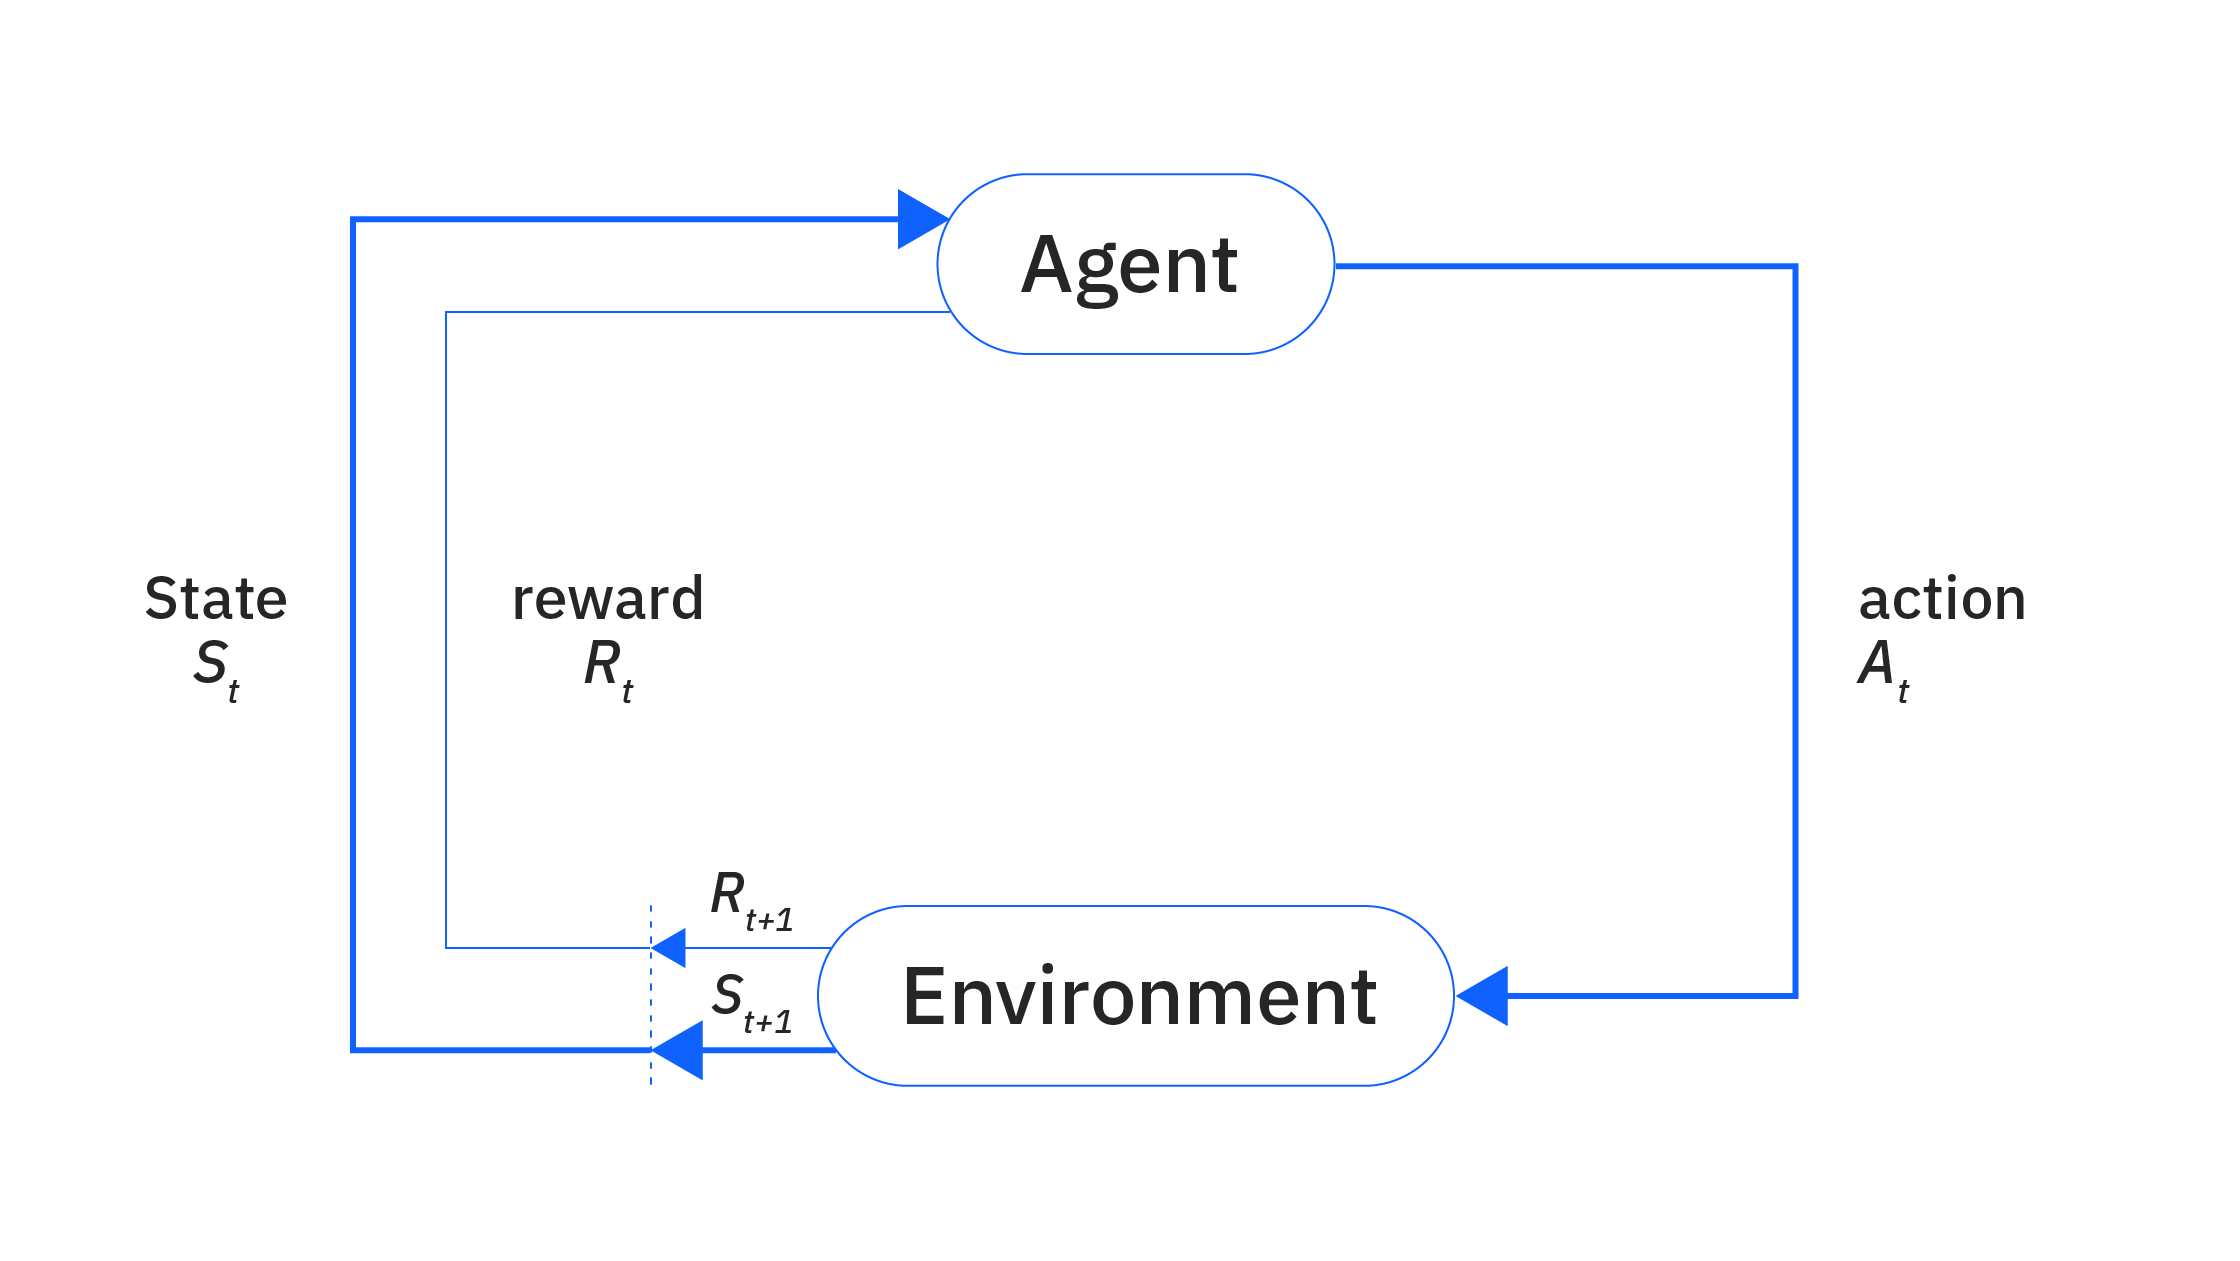
\includegraphics[width=0.8\textwidth]{img/RL_components.png}
    \caption{Vòng lặp học tập của Reinforcement Learning \cite{IBM2024}}
    \label{fig:RL-components}
\end{figure*}
Quá trình học của \ac{rl} diễn ra theo một vòng lặp liên tục:

\begin{enumerate}
    \item Tác nhân quan sát trạng thái hiện tại $s_{t}$ của môi trường.

    \item Dựa trên trạng thái $s_{t}$, tác nhân chọn một hành động $a_{t}$.

    \item Tác nhân thực hiện hành động $a_{t}$.

    \item Môi trường chuyển sang trạng thái mới $s_{t+1}$ và trả về một phần thưởng        $r_{t+1}$ cho tác nhân.

    \item Tác nhân sử dụng thông tin về phần thưởng và trạng thái mới để cập nhật kiến thức của mình, nhằm đưa ra quyết định tốt hơn trong tương lai.
\end{enumerate}

\subsubsection{Đặc điểm khác biệt so với các phương pháp học máy khác}
\ac{rl} khác biệt cơ bản với hai nhánh còn lại của học máy:
\begin{itemize}
    \item \textbf{So với Học có giám sát (Supervised Learning):} Học có giám sát
        học từ một tập dữ liệu đã được gán nhãn sẵn. Ngược lại, trong \ac{rl},
        không có "câu trả lời đúng" cho mỗi trạng thái; tác nhân phải tự tìm ra hành
        động tối ưu. Tín hiệu phản hồi (phần thưởng) cũng có thể bị trễ, không nhất
        thiết phải có ngay sau mỗi hành động.

    \item \textbf{So với Học không giám sát (Unsupervised Learning):} Học không
        giám sát tìm kiếm cấu trúc tiềm ẩn trong dữ liệu không có nhãn. \ac{rl}
        khác ở chỗ nó có một mục tiêu rõ ràng là tối đa hóa phần thưởng, trong khi
        học không giám sát thường không có một mục tiêu tối ưu hóa cụ thể.
\end{itemize}

\subsubsection{Các thuật toán cơ bản}
Các thuật toán \ac{rl} có thể được phân loại thành các nhóm chính như dựa trên giá
trị (Value-Based), dựa trên chiến lược (Policy-Based), và lai ghép Tác nhân-Phê bình
(Actor-Critic).

\subsection{Q-Learning}
\subsubsection{Định nghĩa Q-Learning}
Q-Learning là một thuật toán \ac{rl} kinh điển, thuộc nhóm dựa trên giá trị và không
cần mô hình (model-free). "Không cần mô hình" có nghĩa là tác nhân không cần
hiểu đầy đủ về các quy tắc vận hành của môi trường. Thay vào đó, nó học trực
tiếp từ kinh nghiệm tương tác.

\subsubsection{Hàm giá trị Q}
Trọng tâm của Q-Learning là học một hàm giá trị hành động, gọi là hàm Q-function,
ký hiệu là $Q(s, a)$. Hàm này ước tính tổng phần thưởng chiết khấu trong tương lai
(còn gọi là giá trị Q) mà tác nhân sẽ nhận được nếu nó thực hiện hành động $a$ từ
trạng thái $s$, và sau đó tuân theo chiến lược tối ưu.

\subsubsection{Cơ chế cập nhật giá trị Q và Phương trình Bellman}
Trong các bài toán có không gian trạng thái và hành động nhỏ, hàm Q có thể được lưu
trong một bảng (Q-table). Các giá trị trong bảng được khởi tạo ngẫu nhiên và cập
nhật lặp đi lặp lại bằng phương trình tối ưu Bellman:
\begin{equation}
    Q(s_{t}, a_{t}) \leftarrow Q(s_{t}, a_{t}) + \alpha [r_{t+1}+ \gamma \max_{a}
    Q(s_{t+1}, a) - Q(s_{t}, a_{t})]
\end{equation}
Trong đó, $(r_{t+1}+ \gamma \max_{a}Q(s_{t+1}, a))$ là "giá trị mục tiêu" (target)
mà $Q(s_{t}, a_{t})$ đang cố gắng học.

\subsubsection{Ưu và nhược điểm}
\begin{itemize}
    \item \textbf{Ưu điểm:} Q-Learning đơn giản, dễ triển khai và được chứng minh
        là sẽ hội tụ đến chiến lược tối ưu nếu mỗi cặp (trạng thái, hành động)
        được ghé thăm đủ nhiều lần.

    \item \textbf{Nhược điểm:} Hạn chế lớn nhất của Q-Learning là "lời nguyền của
        chiều dữ liệu". Khi số lượng trạng thái hoặc hành động quá lớn, Q-table
        sẽ trở nên cồng kềnh, đòi hỏi bộ nhớ khổng lồ và thời gian học rất lâu.
        Nó cũng không thể xử lý các không gian trạng thái hoặc hành động liên
        tục.
\end{itemize}

\subsection{Học tăng cường sâu (Deep Reinforcement Learning)}
\subsubsection{Tích hợp mạng nơ-ron với RL}
Học tăng cường sâu (\ac{drl}) ra đời để giải quyết bài toán về chiều dữ liệu của
\ac{rl} truyền thống. Thay vì dùng Q-table, \ac{drl} sử dụng một mạng nơ-ron sâu
(Deep Neural Network - \ac{dnn}) để xấp xỉ hàm giá trị (như Q-function) hoặc trực
tiếp hàm chiến lược \cite{Mnih2015}.

\subsubsection{Kiến trúc mạng nơ-ron và ưu điểm}
Mạng nơ-ron nhận đầu vào là trạng thái của môi trường và đưa ra đầu ra là giá trị
Q cho mỗi hành động hoặc một phân phối xác suất trên các hành động. Ưu điểm
chính của việc tích hợp này là:
\begin{itemize}
    \item \textbf{Khả năng khái quát hóa:} Mạng nơ-ron có thể đưa ra dự đoán cho
        cả những trạng thái chưa từng gặp, dựa trên sự tương đồng với các trạng thái
        đã học.

    \item \textbf{Xử lý đầu vào phức tạp:} \ac{drl} có thể học trực tiếp từ dữ liệu
        thô, có chiều dữ liệu cao như hình ảnh, mà không cần trích xuất đặc trưng
        thủ công.
\end{itemize}

\subsubsection{Các framework phổ biến}
Việc triển khai các thuật toán \ac{drl} được hỗ trợ bởi nhiều framework mạnh mẽ như
TensorFlow, PyTorch, và các thư viện chuyên dụng như Stable Baselines3, RLlib.

\subsection{Deep Q-Learning}
\subsubsection{Nguyên lý hoạt động}
Deep Q-Learning (hay \ac{dqn}) là thuật toán kết hợp trực tiếp ý tưởng của Q-Learning
với mạng nơ-ron sâu \ac{dnn}. Nguyên lý hoạt động của nó là biến bài toán tìm giá
trị Q tối ưu thành một bài toán học có giám sát.

Mạng nơ-ron, được gọi là Q-network, sẽ nhận đầu vào là trạng thái $s$ và đầu ra là
một vector các giá trị Q, mỗi giá trị tương ứng với một hành động có thể thực
hiện $Q(s, \cdot; \theta)$, trong đó $\theta$ là các trọng số của mạng. Quá
trình huấn luyện nhằm điều chỉnh các trọng số $\theta$ sao cho giá trị
$Q(s, a; \theta)$ do mạng dự đoán ngày càng gần với giá trị mục tiêu $y$:
\begin{equation}
    y = r + \gamma \max_{a'}Q(s', a'; \theta)
    \label{eq:q_value}
\end{equation}
Sự chênh lệch giữa giá trị dự đoán và giá trị mục tiêu được đo bằng một hàm mất mát,
thường là Sai số bình phương trung bình (Mean Squared Error - MSE). Sau đó,
thuật toán lan truyền ngược (backpropagation) và hạ gradient (gradient descent)
được sử dụng để cập nhật các trọng số $\theta$ nhằm tối thiểu hóa hàm mất mát
này.

\subsubsection{Kiến trúc mạng và các kỹ thuật ổn định hóa}
Việc thay thế Q-table bằng mạng nơ-ron một cách trực tiếp có thể gây ra sự mất
ổn định trong huấn luyện. \ac{dqn} giới thiệu hai kỹ thuật để giải quyết
vấn đề này:
\begin{itemize}
    \item \textbf{Experience Replay (Bộ nhớ tái hiện kinh nghiệm):} Tác nhân lưu
        trữ các kinh nghiệm $(s, a, r, s')$ vào một bộ nhớ đệm. Thay vì học từ kinh
        nghiệm gần nhất, nó lấy một lô dữ liệu nhỏ ngẫu nhiên từ bộ nhớ để huấn
        luyện. Điều này giúp phá vỡ sự tương quan giữa các mẫu dữ liệu liên tiếp,
        làm cho quá trình học ổn định hơn.

    \item \textbf{Target Network (Mạng mục tiêu):} \ac{dqn} sử dụng hai mạng:
        một mạng chính được cập nhật liên tục và một mạng mục tiêu được giữ cố
        định. Mạng mục tiêu được dùng để tính toán giá trị Q mục tiêu, tạo ra
        một "đích đến" ổn định cho mạng chính học theo. Trọng số của mạng mục tiêu
        được sao chép từ mạng chính sau một số bước nhất định.
\end{itemize}

\subsubsection{Các biến thể và phát triển}
Kể từ khi ra đời, \ac{dqn} đã có nhiều biến thể cải tiến quan trọng, ví dụ:
\begin{itemize}
    \item \textbf{Double DQN:} Giảm thiểu việc đánh giá quá cao các giá trị Q, giúp
        quá trình học ổn định và chính xác hơn.

    \item \textbf{Dueling DQN:} Sử dụng một kiến trúc mạng đặc biệt, tách biệt việc
        ước tính giá trị của trạng thái (state value) và lợi thế của từng hành động
        (action advantage), giúp học hiệu quả hơn.
\end{itemize}

% \subsection{Soft Actor-Critic}
% \subsubsection{Tổng quan về Soft Actor-Critic}
% Soft Actor-Critic (\ac{sac}) là một thuật toán học tăng cường sâu hiện đại, thuộc nhóm Actor-Critic và được thiết kế đặc biệt cho các bài toán có không gian hành động liên tục \cite{Haarnoja2018}. Khác với \ac{dqn} chỉ phù hợp với hành động rời rạc, \ac{sac} có thể xử lý các hành động có giá trị liên tục, điều này rất quan trọng trong nhiều ứng dụng thực tế như điều khiển robot, tự động hóa, và điều phối hệ thống.

% \subsubsection{Nguyên lý Maximum Entropy}
% Điểm đặc biệt của \ac{sac} là việc áp dụng nguyên lý Maximum Entropy trong quá trình học. Thay vì chỉ tối đa hóa phần thưởng tích lũy như các thuật toán truyền thống, \ac{sac} đồng thời tối đa hóa entropy của policy:

% \begin{equation}
%     J(\pi) = \sum_{t=0}^{T} \mathbb{E}_{(s_t,a_t) \sim \rho_\pi} [r(s_t, a_t) + \alpha \mathcal{H}(\pi(\cdot|s_t))]
% \end{equation}

% Trong đó $\mathcal{H}(\pi(\cdot|s_t))$ là entropy của policy tại trạng thái $s_t$, và $\alpha$ là hệ số cân bằng giữa reward và entropy. Việc tối đa hóa entropy giúp:
% \begin{itemize}
%     \item \textbf{Khuyến khích khám phá:} Policy được khuyến khích duy trì tính ngẫu nhiên, giúp tác nhân khám phá môi trường hiệu quả hơn
%     \item \textbf{Tránh hội tụ sớm:} Ngăn chặn policy hội tụ quá sớm về một giải pháp cục bộ
%     \item \textbf{Tăng tính ổn định:} Cải thiện độ ổn định trong quá trình huấn luyện
% \end{itemize}

% \subsubsection{Kiến trúc Actor-Critic}
% \ac{sac} sử dụng kiến trúc Actor-Critic với các thành phần chính:
% \begin{itemize}
%     \item \textbf{Actor (Policy Network):} Học một policy stochastic $\pi_\phi(a|s)$ để chọn hành động. Actor được huấn luyện để tối đa hóa cả reward và entropy
%     \item \textbf{Critic (Q-Networks):} Sử dụng hai mạng Q song song $Q_{\theta_1}(s,a)$ và $Q_{\theta_2}(s,a)$ để ước lượng giá trị Q. Việc sử dụng hai mạng giúp giảm thiểu sai lệch ước lượng quá mức (overestimation bias)
%     \item \textbf{Target Networks:} Sử dụng target networks cho cả Actor và Critic để ổn định quá trình huấn luyện
% \end{itemize}

% \subsubsection{Thuật toán huấn luyện}
% Quá trình huấn luyện \ac{sac} bao gồm các bước chính:
% \begin{enumerate}
%     \item \textbf{Cập nhật Critic:} Hai mạng Q được huấn luyện để tối thiểu hóa Bellman error:
%     \begin{equation}
%         L_Q = \mathbb{E}_{(s,a,r,s') \sim \mathcal{D}} \left[ (Q_\theta(s,a) - y)^2 \right]
%     \end{equation}
%     với $y = r + \gamma \mathbb{E}_{a' \sim \pi} [Q_{\bar{\theta}}(s',a') - \alpha \log \pi(a'|s')]$
    
%     \item \textbf{Cập nhật Actor:} Policy được cập nhật để tối đa hóa expected Q-value và entropy:
%     \begin{equation}
%         L_\pi = \mathbb{E}_{s \sim \mathcal{D}, a \sim \pi} [\alpha \log \pi(a|s) - Q_\theta(s,a)]
%     \end{equation}
    
%     \item \textbf{Điều chỉnh temperature parameter:} Hệ số $\alpha$ có thể được tự động điều chỉnh để cân bằng giữa exploration và exploitation
% \end{enumerate}

% \subsubsection{Ưu điểm của SAC}
% \ac{sac} có nhiều ưu điểm vượt trội:
% \begin{itemize}
%     \item \textbf{Hiệu quả dữ liệu:} Học hiệu quả với ít dữ liệu hơn so với các thuật toán dựa trên policy
%     \item \textbf{Ổn định:} Ít nhạy cảm với siêu tham số (hyperparameter) và ổn định trong quá trình huấn luyện
%     \item \textbf{Khả năng khám phá tốt:} Maximum entropy giúp duy trì khả năng khám phá trong suốt quá trình học
%     \item \textbf{Phù hợp với hành động liên tục:} Được thiết kế đặc biệt cho không gian hành động liên tục
% \end{itemize}

\subsection{Soft Actor-Critic}
\subsubsection{Tổng quan về Soft Actor-Critic}
Soft Actor-Critic (\ac{sac}) là một thuật toán học tăng cường sâu hiện đại, thuộc nhóm Actor-Critic và được thiết kế đặc biệt cho các bài toán có không gian hành động liên tục \cite{Haarnoja2018}. Khác với \ac{dqn} chỉ phù hợp với hành động rời rạc, \ac{sac} có thể xử lý các hành động có giá trị liên tục, điều này rất quan trọng trong nhiều ứng dụng thực tế như điều khiển robot, tự động hóa, và điều phối hệ thống.

\subsubsection{Nguyên lý Maximum Entropy}
Điểm đặc biệt của \ac{sac} là việc áp dụng nguyên lý Maximum Entropy trong quá trình học. Thay vì chỉ tối đa hóa phần thưởng tích lũy như các thuật toán truyền thống, \ac{sac} đồng thời tối đa hóa entropy của policy:

\begin{equation}
    J(\pi) = \sum_{t=0}^{T} \mathbb{E}_{(s_t,a_t) \sim \rho_\pi} [r(s_t, a_t) + \alpha \mathcal{H}(\pi(\cdot|s_t))]
\end{equation}

Trong đó $\mathcal{H}(\pi(\cdot|s_t))$ là entropy của policy tại trạng thái $s_t$, và $\alpha$ là hệ số cân bằng giữa reward và entropy. Việc tối đa hóa entropy giúp:
\begin{itemize}
    \item \textbf{Khuyến khích khám phá:} Policy được khuyến khích duy trì tính ngẫu nhiên, giúp tác nhân khám phá môi trường hiệu quả hơn
    \item \textbf{Tránh hội tụ sớm:} Ngăn chặn policy hội tụ quá sớm về một giải pháp cục bộ
    \item \textbf{Tăng tính ổn định:} Cải thiện độ ổn định trong quá trình huấn luyện
\end{itemize}

\subsubsection{Kiến trúc Actor-Critic}
\ac{sac} sử dụng kiến trúc Actor-Critic với các thành phần chính:
\begin{itemize}
    \item \textbf{Actor (Policy Network):} Học một policy stochastic $\pi_\phi(a|s)$ để chọn hành động. Actor được huấn luyện để tối đa hóa cả reward và entropy
    \item \textbf{Critic (Q-Networks):} Sử dụng hai mạng Q song song $Q_{\theta_1}(s,a)$ và $Q_{\theta_2}(s,a)$ để ước lượng giá trị Q. Việc sử dụng hai mạng giúp giảm thiểu sai lệch ước lượng quá mức (overestimation bias)
    \item \textbf{Target Networks:} Sử dụng target networks cho cả Actor và Critic để ổn định quá trình huấn luyện
\end{itemize}

\subsubsection{Thuật toán huấn luyện}
Quá trình huấn luyện \ac{sac} bao gồm các bước chính:
\begin{enumerate}
    \item \textbf{Cập nhật Critic:} Hai mạng Q được huấn luyện để tối thiểu hóa Bellman error:
    \begin{equation}
        L_Q = \mathbb{E}_{(s,a,r,s') \sim \mathcal{D}} \left[ (Q_\theta(s,a) - y)^2 \right]
    \end{equation}
    với $y = r + \gamma \mathbb{E}_{a' \sim \pi} [Q_{\bar{\theta}}(s',a') - \alpha \log \pi(a'|s')]$
    
    \item \textbf{Cập nhật Actor:} Policy được cập nhật để tối đa hóa expected Q-value và entropy:
    \begin{equation}
        L_\pi = \mathbb{E}_{s \sim \mathcal{D}, a \sim \pi} [\alpha \log \pi(a|s) - Q_\theta(s,a)]
    \end{equation}
    
    \item \textbf{Điều chỉnh temperature parameter:} Hệ số $\alpha$ có thể được tự động điều chỉnh để cân bằng giữa exploration và exploitation
\end{enumerate}

\subsubsection{Ưu điểm của SAC}
\ac{sac} có nhiều ưu điểm vượt trội:
\begin{itemize}
    \item \textbf{Hiệu quả dữ liệu:} Học hiệu quả với ít dữ liệu hơn so với các thuật toán dựa trên policy
    \item \textbf{Ổn định:} Ít nhạy cảm với siêu tham số (hyperparameter) và ổn định trong quá trình huấn luyện
    \item \textbf{Khả năng khám phá tốt:} Maximum entropy giúp duy trì khả năng khám phá trong suốt quá trình học
    \item \textbf{Phù hợp với hành động liên tục:} Được thiết kế đặc biệt cho không gian hành động liên tục
\end{itemize}

\section{Thuật toán nhận diện vật thể YOLO}
\subsection{Tổng quan về YOLO}
YOLO (You Only Look Once) là một thuật toán phát hiện đối tượng theo thời gian thực,
được giới thiệu lần đầu tiên vào năm 2015. Khác với các phương pháp phát hiện
đối tượng truyền thống sử dụng phương pháp hai giai đoạn (two-stage detection), YOLO
xử lý phát hiện đối tượng như một vấn đề hồi quy đơn lẻ, dự đoán các hộp giới
hạn và xác suất lớp trực tiếp từ hình ảnh đầy đủ trong một lần đánh giá
\cite{Redmon2016}. Phương pháp này giúp YOLO đạt được tốc độ xử lý nhanh hơn đáng
kể so với các phương pháp trước đó.

\subsection{Nguyên lý hoạt động}
YOLO áp dụng cách tiếp cận khác biệt trong bài toán phát hiện đối tượng so với các phương pháp truyền thống, khi xử lý toàn bộ hình ảnh chỉ trong một lần duy nhất thay vì chia nhỏ và xử lý trên từng vùng. Hình \ref{fig:yolo_architecture} minh họa cách thức hoạt động của thuật toán này.

\begin{figure}[!htp]
    \centering
    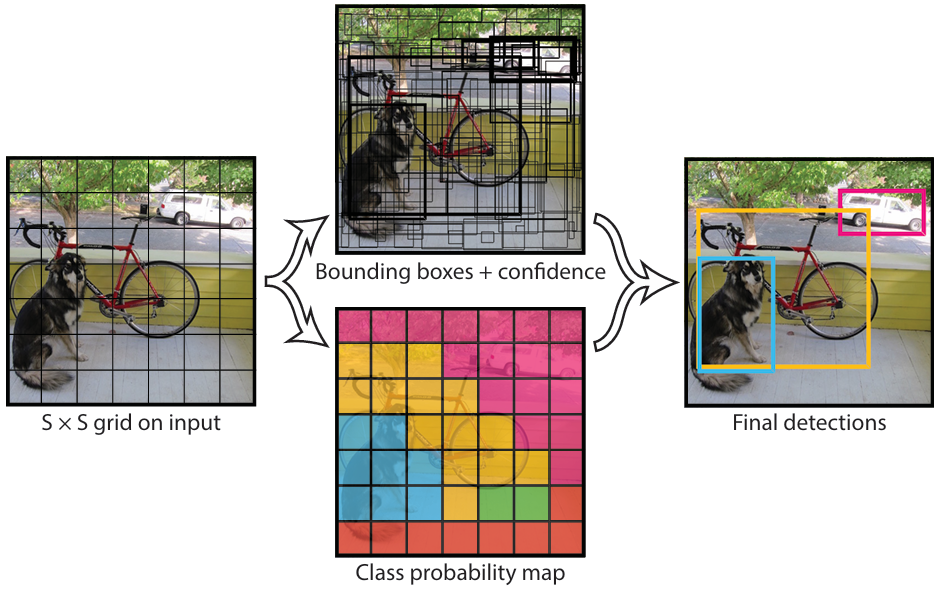
\includegraphics[width=0.6\textwidth]{img/yolo_1}
    \caption{Nguyên lý hoạt động của YOLO}
    \label{fig:yolo_architecture}
\end{figure}

Cụ thể, thuật toán chia hình ảnh đầu vào thành một lưới $S \times S$ cells. Mỗi cell chịu
trách nhiệm dự đoán các đối tượng có tâm nằm trong nó. Mỗi cell dự đoán:
\begin{itemize}
    \item $B$ bounding boxes và độ tin cậy (confidence scores) cho mỗi box

    \item $C$ xác suất có điều kiện của các lớp đối tượng
\end{itemize}

Mỗi bounding box bao gồm 5 thành phần dự đoán:
\begin{equation}
    (x, y, w, h, confidence)
\end{equation}
Trong đó:
\begin{itemize}
    \item $(x, y)$ là tọa độ tâm của box, tương đối so với ranh giới của cell

    \item $(w, h)$ là chiều rộng và chiều cao của box, tương đối so với kích
        thước toàn bộ hình ảnh

    \item $confidence$ phản ánh độ tin cậy của box và độ chính xác của vị trí box
\end{itemize}

\subsection{Quá trình dự đoán}
Quá trình dự đoán của YOLO bao gồm các bước chính:
\begin{enumerate}
    \item \textbf{Xử lý đầu vào:} Hình ảnh được resize về kích thước cố định và
        chia thành lưới $S \times S$.

    \item \textbf{Trích xuất đặc trưng:} Sử dụng mạng \ac{cnn} để trích xuất các
        đặc trưng từ hình ảnh.

    \item \textbf{Dự đoán:} Mỗi cell dự đoán $B$ bounding boxes và xác suất lớp.

    \item \textbf{Lọc kết quả:} Áp dụng ngưỡng confidence và Non-Maximum
        Suppression (NMS) để loại bỏ các dự đoán trùng lặp.
\end{enumerate}

\section{Môi trường mô phỏng giao thông đô thị SUMO}
\ac{sumo}~\footnote{SUMO - Simulation of Urban MObility: \url{https://www.eclipse.org/sumo/}} (Simulation of Urban MObility) là một bộ phần mềm giả lập giao thông vi
mô, mã nguồn mở, và đa nền tảng, được phát triển bởi Trung tâm Hàng không Vũ trụ
Đức. Mục tiêu chính của \ac{sumo} là cung cấp một công cụ mạnh mẽ và linh hoạt
để nghiên cứu các hệ thống giao thông, cho phép các nhà nghiên cứu, kỹ sư và nhà
hoạch định chính sách mô hình hóa, phân tích và đánh giá các kịch bản giao thông
khác nhau mà không cần triển khai trong thế giới thực.

Là một công cụ giả lập vi mô, \ac{sumo} mô hình hóa từng phương tiện riêng lẻ trong
mạng lưới. Mỗi phương tiện có các thuộc tính và hành vi riêng (ví dụ: mô hình
bám đuôi xe, mô hình chuyển làn), và sự tương tác của chúng tạo nên các hiện tượng
giao thông vĩ mô như tắc nghẽn. Điều này làm cho \ac{sumo} trở thành một môi trường
lý tưởng để thử nghiệm các thuật toán điều khiển giao thông thông minh, đặc biệt
là các phương pháp dựa trên \ac{drl}, nơi tác nhân cần một môi trường chi tiết
để học hỏi và tương tác.

\subsection{Các thành phần và kiến trúc cốt lõi}
Một kịch bản giả lập trong \ac{sumo} thường bao gồm ba loại tệp chính:
\begin{itemize}
    \item Mạng lưới giao thông

    \item Nhu cầu giao thông

    \item Cấu hình giả lập
\end{itemize}

\subsubsection{Mạng lưới giao thông (Network)}
Mạng lưới định nghĩa cơ sở hạ tầng đường bộ, được lưu trong tệp có phần mở rộng
\texttt{.net.xml}. Nó bao gồm:
\begin{itemize}
    \item \textbf{Nodes (Nút):} Đại diện cho các nút giao thông hoặc các điểm
        cuối của một con đường.

    \item \textbf{Edges (Cạnh):} Đại diện cho các đoạn đường kết nối các nút. Mỗi
        cạnh có các thuộc tính như số làn, giới hạn tốc độ, và quyền ưu tiên.

    \item \textbf{Traffic Lights (Đèn tín hiệu):} Logic điều khiển tại các nút
        giao, bao gồm các pha và thời gian của chúng.
\end{itemize}
\ac{sumo} cung cấp công cụ \texttt{netedit}, một trình soạn thảo đồ họa, cho phép
người dùng dễ dàng tạo và chỉnh sửa các mạng lưới này. Ngoài ra, \ac{sumo} cũng
có thể nhập mạng lưới từ các nguồn dữ liệu thực tế như OpenStreetMap.

\subsubsection{Nhu cầu giao thông (Demand)}
Nhu cầu giao thông mô tả các phương tiện và hành trình của chúng trong mạng lưới,
thường được định nghĩa trong tệp \texttt{.rou.xml}. Các thành phần chính bao gồm:
\begin{itemize}
    \item \textbf{Vehicle Types (Loại phương tiện):} Định nghĩa các đặc tính vật
        lý và hành vi của phương tiện, chẳng hạn như chiều dài, gia tốc tối đa, giảm
        tốc, và cả mô hình hành vi của người lái xe (ví dụ: mức độ "hoàn hảo"
        của tài xế).

    \item \textbf{Routes (Tuyến đường):} Là một chuỗi các cạnh mà một phương
        tiện sẽ đi qua.

    \item \textbf{Flows (Luồng phương tiện):} Cho phép định nghĩa một lượng lớn
        phương tiện được tạo ra theo thời gian, thay vì phải định nghĩa từng chiếc
        xe một. Điều này rất hữu ích để mô phỏng các kịch bản giao thông thực tế
        với lưu lượng lớn.
\end{itemize}

\subsubsection{Cấu hình giả lập (Configuration)}
Tệp cấu hình, thường có đuôi \texttt{.sumocfg}, là tệp chính để chạy một kịch
bản giả lập. Nó chỉ định các tệp đầu vào cần thiết (như tệp mạng lưới và tệp nhu
cầu), thời gian bắt đầu và kết thúc của giả lập, và các tùy chọn đầu ra khác.

\subsection{Giao diện điều khiển TraCI (Traffic Control Interface)}
Một trong những tính năng mạnh mẽ nhất của \ac{sumo} là Giao diện Điều khiển
Giao thông (Traffic Control Interface - TraCI). Đây là một giao diện lập trình ứng
dụng (API) hoạt động dựa trên giao thức TCP, cho phép các ứng dụng bên ngoài
tương tác và điều khiển giả lập \ac{sumo} đang chạy theo thời gian thực. TraCI
mở ra khả năng kết nối \ac{sumo} với các kịch bản điều khiển phức tạp, các công
cụ phân tích dữ liệu hoặc các hệ thống phần mềm khác, chẳng hạn như một chương trình
viết bằng Python.

Quá trình tương tác thông qua TraCI hoạt động theo một vòng lặp đồng bộ giữa \ac{sumo}
và ứng dụng bên ngoài tại mỗi bước thời gian của giả lập:
\begin{enumerate}
    \item \textbf{Truy xuất dữ liệu (Data Retrieval):} Ứng dụng bên ngoài gửi
        yêu cầu và nhận về dữ liệu chi tiết từ môi trường giả lập. Các dữ liệu này
        có th0ể bao gồm thông tin về các đối tượng trong giả lập (ví dụ: vị trí,
        tốc độ của từng phương tiện) hoặc trạng thái của cơ sở hạ tầng (ví dụ: trạng
        thái đèn tín hiệu, số xe trên một làn đường).

    \item \textbf{Thay đổi trạng thái (State Modification):} Dựa trên dữ liệu
        thu được và logic của ứng dụng, nó có thể gửi các lệnh để thay đổi trạng
        thái của các đối tượng hoặc cơ sở hạ tầng trong giả lập. Ví dụ, một kịch
        bản có thể thay đổi tuyến đường của một phương tiện một cách linh động hoặc
        điều chỉnh chu kỳ đèn tín hiệu của một nút giao.

    \item \textbf{Tiến trình giả lập (Simulation Step):} Sau khi ứng dụng bên
        ngoài hoàn tất việc trao đổi dữ liệu, nó sẽ gửi một lệnh cho \ac{sumo}
        để tiến hành giả lập trong một khoảng thời gian ngắn (ví dụ, một giây).
        \ac{sumo} sẽ tạm dừng sau khi hoàn thành bước này và chờ lệnh tiếp theo,
        đảm bảo quá trình được đồng bộ.
\end{enumerate}
Cơ chế tương tác linh hoạt này cho phép triển khai và kiểm thử các thuật toán điều
khiển giao thông thích ứng, các chiến lược định tuyến động, hoặc thu thập dữ liệu
chi tiết cho các mục đích phân tích mà không bị giới hạn bởi các chức năng có sẵn
của \ac{sumo}. Điều này làm cho \ac{sumo} kết hợp với TraCI trở thành một nền
tảng tiêu chuẩn cho việc nghiên cứu và phát triển các hệ thống giao thông thông
minh.

\subsection{Ứng dụng của SUMO}
Nhờ vào tính linh hoạt, khả năng mở rộng và bản chất mã nguồn mở, \ac{sumo} đã được
sử dụng rộng rãi trong hàng ngàn công trình nghiên cứu khoa học trên toàn thế giới.
Dưới đây là một số ví dụ tiêu biểu về ứng dụng của \ac{sumo}:
\begin{itemize}
    \item \textbf{Đánh giá và so sánh các chiến lược điều khiển giao thông:}
        Nhiều nghiên cứu sử dụng \ac{sumo} để tạo ra một môi trường giả lập thực
        tế nhằm so sánh hiệu quả của các phương pháp điều khiển đèn tín hiệu khác
        nhau.

    \item \textbf{Huấn luyện và kiểm thử các thuật toán học tăng cường:} \ac{sumo},
        đặc biệt khi kết hợp với TraCI, đã trở thành một nền tảng tiêu chuẩn để phát
        triển các tác nhân điều khiển giao thông thông minh dựa trên học tăng cường.
        Các nhà nghiên cứu có thể tạo ra các môi trường phức tạp và đa dạng để
        huấn luyện các mô hình \ac{drl} mà không tốn chi phí và rủi ro như thử nghiệm
        trong thế giới thực.

    \item \textbf{Hiệu chỉnh mô phỏng từ dữ liệu thực tế:} Để đảm bảo tính chính
        xác của các kết quả giả lập, nhiều nghiên cứu tập trung vào việc hiệu chỉnh
        các tham số của \ac{sumo} dựa trên dữ liệu thu thập từ thế giới thực.

    \item \textbf{Nghiên cứu về mạng giao tiếp giữa các phương tiện (V2X):} \ac{sumo}
        cũng là một công cụ quan trọng trong lĩnh vực nghiên cứu mạng giao tiếp giữa
        các phương tiện (Vehicular Ad-hoc Networks - VANETs). Bằng cách tích hợp
        \ac{sumo} với các trình giả lập mạng như NS-3 hoặc OMNeT++, các nhà
        nghiên cứu có thể mô phỏng đồng thời cả hành vi di chuyển của phương
        tiện và quá trình trao đổi thông tin giữa chúng. Điều này cho phép đánh giá
        các giao thức định tuyến, các ứng dụng an toàn (ví dụ: cảnh báo va chạm)
        và các hệ thống quản lý giao thông dựa trên giao tiếp V2X trong một môi trường
        tích hợp và thực tế.
\end{itemize}


\chapter{Phương pháp thực hiện}
\label{c:phuongphapthuchien}
Chương này tập trung vào việc mô tả hệ thống điều khiển đèn giao thông thông minh sử dụng thuật toán học tăng cường sâu (\ac{drl}). Hệ thống sẽ được huấn luyện và đánh giá trong môi trường giả lập \ac{sumo}, với dữ liệu đầu vào có thể được thu thập từ thực tế thông qua các camera tích hợp thuật toán nhận diện vật thể \ac{yl}.

\section{Kiến trúc tổng thể hệ thống}
Để có cái nhìn toàn diện về hệ thống điều khiển đèn giao thông thông minh, trước tiên, chúng ta cần tìm hiểu kiến trúc tổng thể của nó. Hệ thống này được thiết kế theo mô hình phân tầng, cho phép khả năng mở rộng linh hoạt từ việc điều khiển một giao lộ đơn lẻ đến việc điều phối đồng bộ nhiều giao lộ cùng lúc.

\subsection{Kiến trúc tổng quan}

\begin{figure*}[!htp]
    \centering
    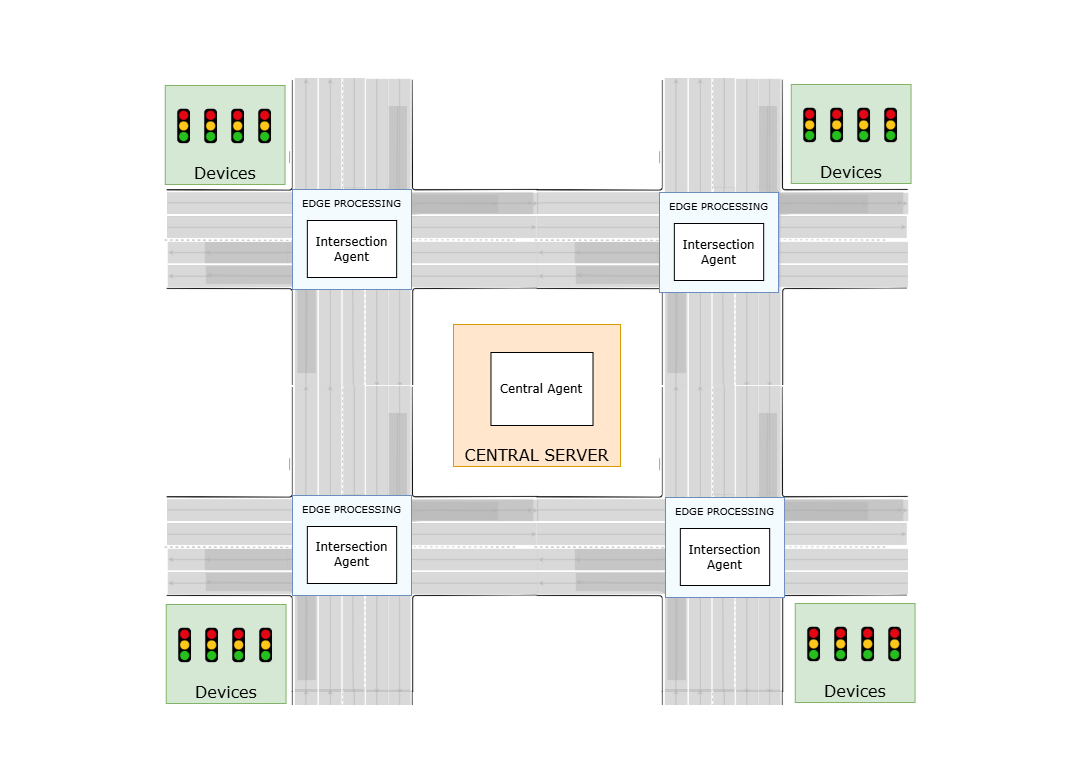
\includegraphics[width=\textwidth]{img/overview_architecture.png}
    \caption{Kiến trúc tổng quan hệ thống điều khiển đèn giao thông thông minh}
    \label{fig:overview_architecture}
\end{figure*}

Hình \ref{fig:overview_architecture} thể hiện kiến trúc tổng quan của hệ thống,
bao gồm các thành phần chính:

\begin{itemize}
    \item \textbf{Lớp thu thập dữ liệu:} Thu thập dữ liệu từ camera và sensors

    \item \textbf{Lớp xử lý:} Xử lý dữ liệu và nhận diện đối tượng

    \item \textbf{Lớp quyết định:} Các agent AI ra quyết định điều khiển

    \item \textbf{Lớp đồng bộ:} Đồng bộ hóa giữa các giao lộ

    \item \textbf{Lớp điều khiển:} Điều khiển đèn giao thông thực tế
\end{itemize}

\subsection{Kiến trúc chi tiết hệ thống}

\begin{figure*}[!htp]
    \centering
    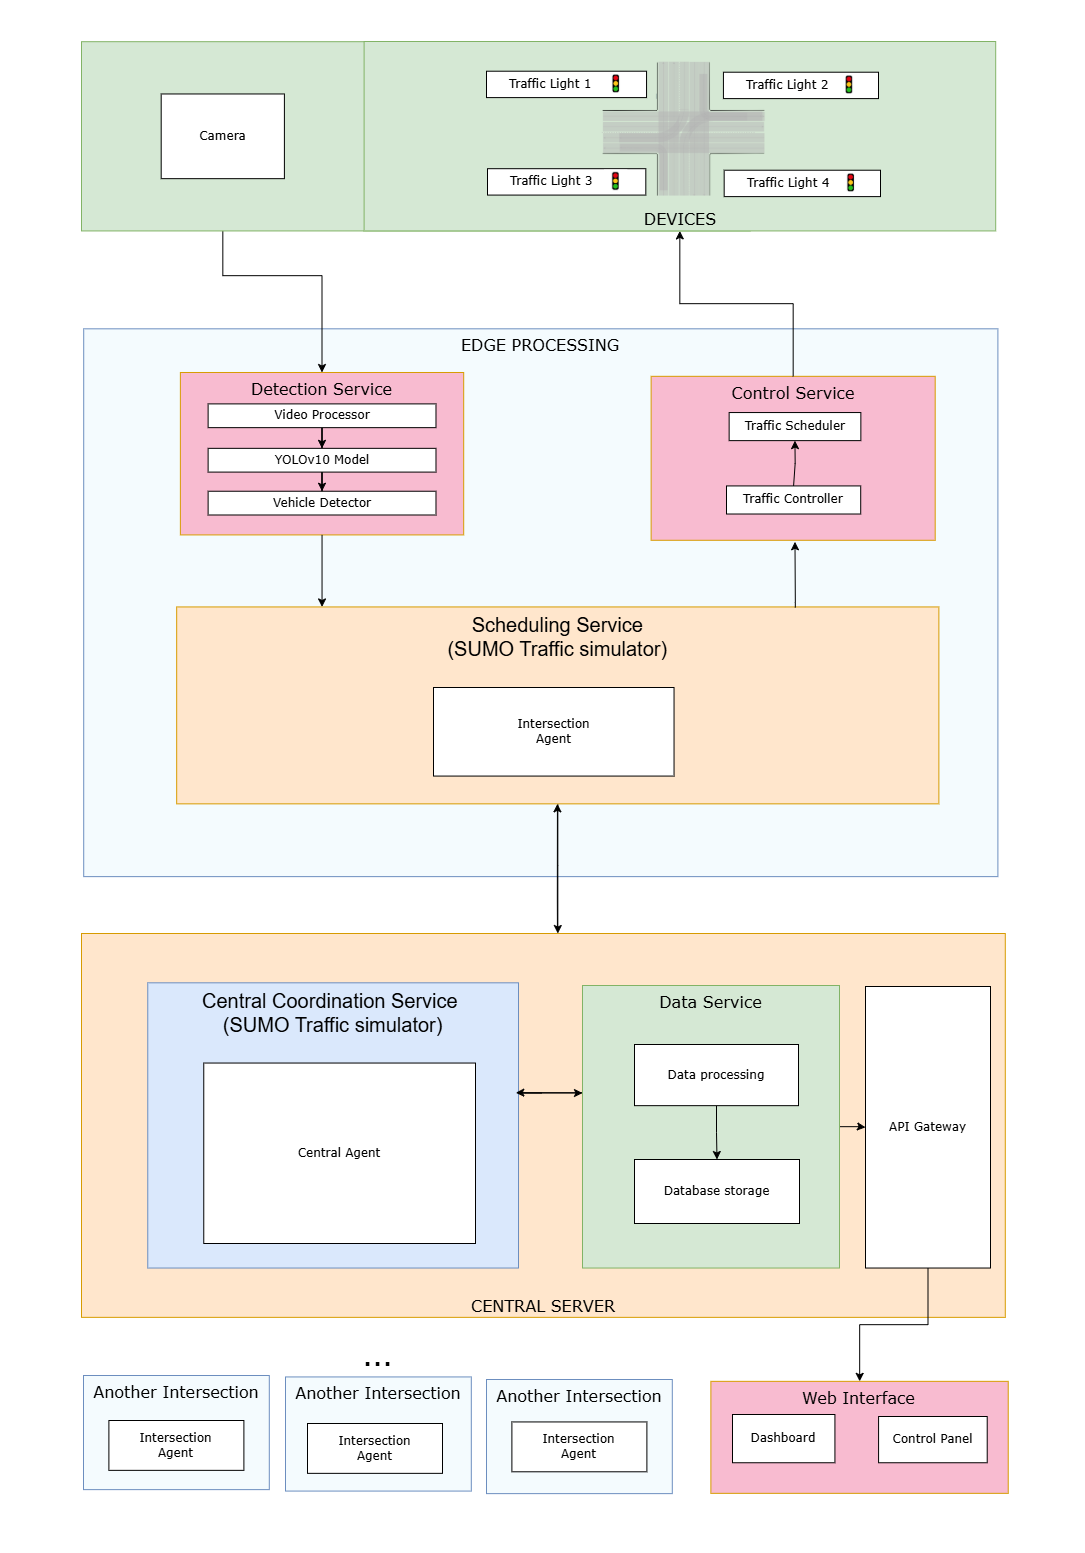
\includegraphics[width=0.7\textwidth]{img/detailed_architecture.png}
    \caption{Kiến trúc chi tiết hệ thống với các thành phần}
    \label{fig:detailed_architecture}
\end{figure*}

Mô tả chi tiết các thành phần và luồng dữ liệu trong hệ thống:

\begin{enumerate}
    \item \textbf{Lớp thiết bị:} Thu thập video từ các camera giám sát giao thông
    \item \textbf{Lớp xử lý biên}
    \begin{itemize}
        \item \textbf{Nhận diện phương tiện tham gia giao thông:} Dữ liệu video sẽ được dùng để nhận diện các phương tiện tham gia giao thông cũng như xác định khoảng cách và làn đường mà phương tiện đang di chuyển
        \item \textbf{Các tác nhân DQN :} Các tác nhân ngoài việc điều khiển đèn tín hiệu từng giao lộ thì còn có nhiệm vụ nhận các thông tin từ YOLO và giả lập tình trạng giao thông tại nút giao. Sau đó, gửi các thông tin cần thiết đến centtral server để dự doán và ra quyết định 
    \end{itemize}
    \item \textbf{Central Server:} Thu thập từ các tác nhân và chạy các mô hình DQN và Sync Agent để ra quyết định. Đồng thời, cung cấp giao diện để quan sát và điều khiển
\end{enumerate}

\section{Phương pháp mô phỏng dữ liệu từ camera}
\subsection{Mô hình nhận diện vật thể}
Để phát hiện và nhận diện phương tiện trong các luồng video giao thông, sử dụng mô hình \textbf{YOLO11}, phiên bản mới nhất trong chuỗi mô hình phát hiện đối tượng thời gian thực của \textbf{Ultralytics}. YOLO11 mang đến những cải tiến đáng kể về kiến trúc và phương pháp huấn luyện, giúp nâng cao độ chính xác, tốc độ và hiệu quả so với các phiên bản tiền nhiệm.

\begin{figure}[!htp]
    \centering
    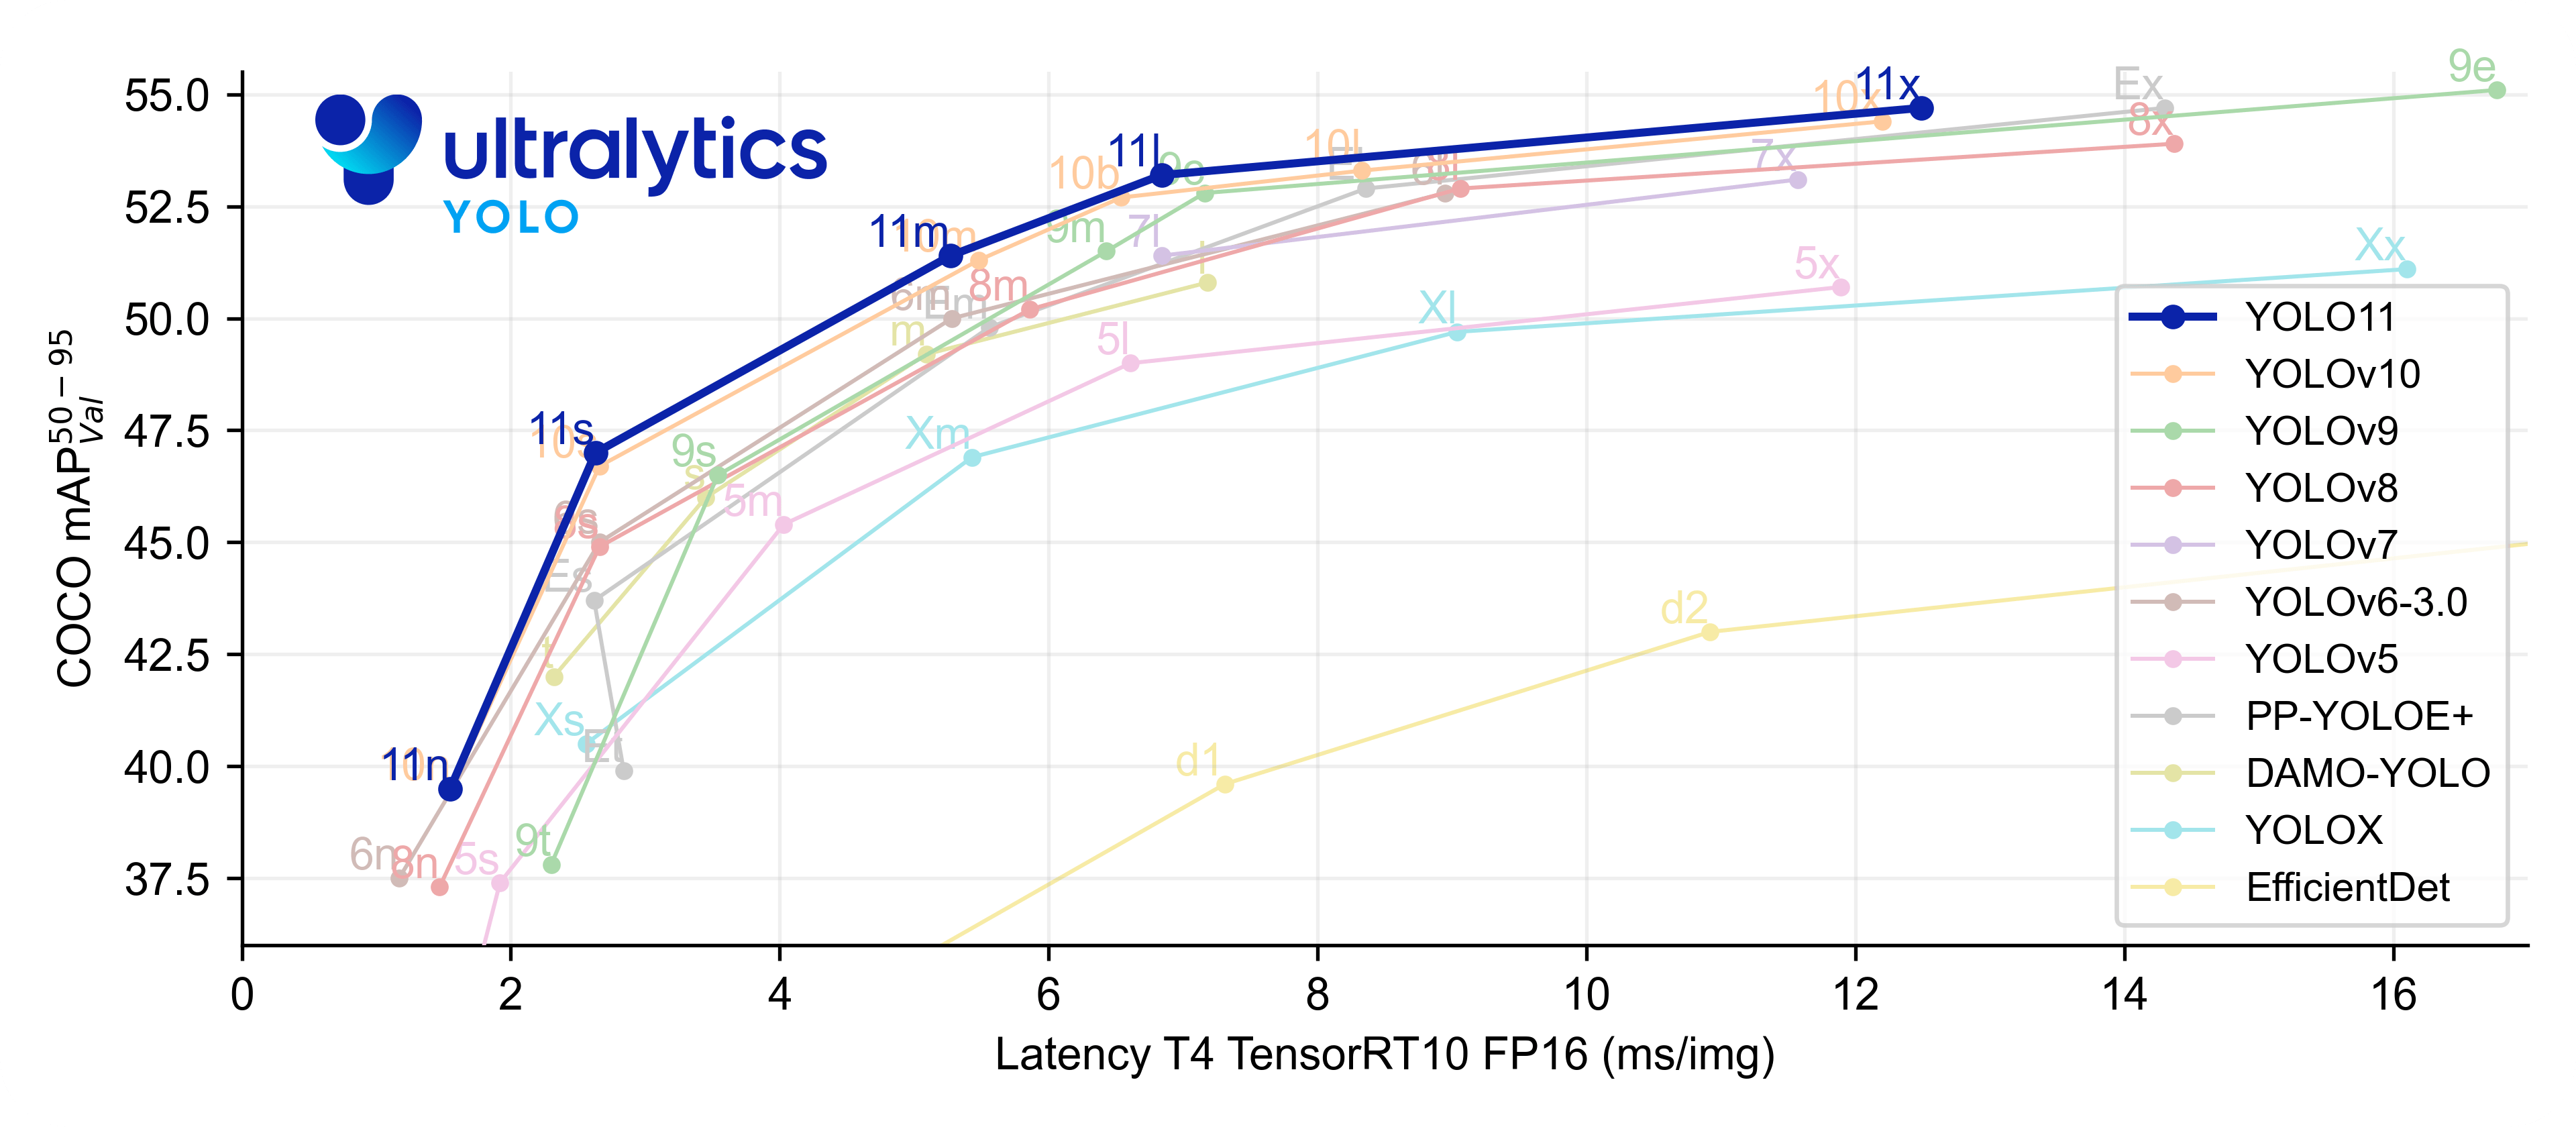
\includegraphics[width=\textwidth]{img/yolo_models}
    \caption{So sánh hiệu suất giữa các mô hình \footnotemark[1]}
    \label{fig:yolo_models}
\end{figure}
Cụ thể, nghiên cứu này sử dụng mô hình đã được huấn luyện trước (pre-trained) có tên là \textbf{\texttt{yolov11s.pt}}. Đây là phiên bản thu nhỏ của YOLO11, được lựa chọn dựa trên các ưu điểm nổi bật sau:

\begin{itemize}
    \item \textbf{Hiệu suất cân bằng:} Mô hình \texttt{yolov11s.pt} đạt được chỉ số mAP\textsuperscript{50-95} là 47.0 trên tập dữ liệu COCO, đồng thời có tốc độ xử lý rất nhanh (chỉ 2.5ms trên GPU Tesla T4). Sự cân bằng giữa độ chính xác cao và tốc độ suy luận nhanh là yếu tố then chốt cho các ứng dụng phân tích giao thông thời gian thực\footnote[1]{Ultralytics Documents: \url{https://docs.ultralytics.com/models/yolo11}}.
    \item \textbf{Kiến trúc hiệu quả:} YOLO11 được cải tiến về kiến trúc backbone và neck, giúp tăng cường khả năng trích xuất đặc trưng. Nhờ đó, các mô hình như YOLO11 đạt được độ chính xác cao hơn với số lượng tham số ít hơn, làm cho chúng hiệu quả hơn về mặt tính toán. Phiên bản \texttt{yolov11s.pt} chỉ có 9.4 triệu tham số.
    \item \textbf{Huấn luyện trên tập dữ liệu COCO:} Giống như các phiên bản trước, mô hình được huấn luyện sẵn trên tập dữ liệu COCO, bao gồm các lớp đối tượng giao thông quan trọng như \texttt{car}, \texttt{motorcycle}, \texttt{bus}, và \texttt{truck}. Điều này cho phép áp dụng mô hình trực tiếp vào bài toán mà không cần huấn luyện lại, giúp tiết kiệm thời gian và tài nguyên.
\end{itemize}
Với những lý do trên, mô hình \texttt{yolov11s.pt} được xác định là lựa chọn phù hợp nhất, đáp ứng được các yêu cầu về độ chính xác, tốc độ và hiệu quả cho hệ thống được đề xuất trong luận văn.

\subsection{Thuật toán theo dõi đối tượng}
\subsubsection{SORT}
SORT (Simple Online and Realtime Tracking) là một thuật toán theo dõi đối tượng đơn giản nhưng hiệu quả. Thuật toán này kết hợp giữa bộ lọc Kalman và thuật toán Hungarian để theo dõi các đối tượng qua nhiều khung hình video liên tiếp. Trong nghiên cứu này, SORT được sử dụng để theo dõi các phương tiện giao thông qua các khung hình video, giúp duy trì ID nhất quán cho mỗi phương tiện và thu thập thông tin về quỹ đạo di chuyển của chúng. SORT hoạt động theo các bước chính sau:

\begin{itemize}
    \item \textbf{Dự đoán vị trí:} Sử dụng bộ lọc Kalman để dự đoán vị trí của các đối tượng đã được theo dõi trong khung hình tiếp theo. Bộ lọc này mô hình hóa chuyển động của đối tượng dựa trên vận tốc và gia tốc.

    \item \textbf{Gán đối tượng:} Khi nhận được các phát hiện mới từ mô hình YOLO, SORT sử dụng thuật toán Hungarian để gán các phát hiện này với các đối tượng đang được theo dõi. Việc gán dựa trên khoảng cách IoU (Intersection over Union) giữa các hộp giới hạn dự đoán và phát hiện.

    \item \textbf{Cập nhật trạng thái:} Sau khi gán thành công, bộ lọc Kalman được cập nhật với thông tin mới từ các phát hiện. Các đối tượng không được gán trong một số khung hình liên tiếp sẽ bị loại bỏ khỏi danh sách theo dõi.
\end{itemize}

Ưu điểm chính của SORT là:
\begin{itemize}
    \item \textbf{Tốc độ xử lý cao:} Thuật toán có thể xử lý video với tốc độ khung hình cao, phù hợp cho các ứng dụng thời gian thực.

    \item \textbf{Độ chính xác tốt:} Đạt được độ chính xác cao trong việc theo dõi các đối tượng chuyển động với tốc độ vừa phải.

    \item \textbf{Tính đơn giản:} Dễ dàng triển khai và tích hợp với các mô hình phát hiện đối tượng khác nhau.
\end{itemize}

Tuy nhiên, SORT cũng có một số hạn chế:
\begin{itemize}
    \item \textbf{Không xử lý tốt các trường hợp che khuất:} Khi đối tượng bị che khuất hoàn toàn trong một khoảng thời gian, thuật toán có thể mất dấu đối tượng đó.

    \item \textbf{Không duy trì ID khi đối tượng tái xuất hiện:} Nếu một đối tượng biến mất và xuất hiện lại, nó sẽ được gán một ID mới.
\end{itemize}

\subsubsection{BotSORT}
BotSORT (Boosting SORT) là một phiên bản cải tiến của thuật toán SORT, được tích hợp trong thư viện Ultralytics. Đây là thuật toán chính được dùng trong nghiên cứu, thuật toán này khắc phục các hạn chế của SORT bằng cách bổ sung thêm các tính năng:

\begin{itemize}
    \item \textbf{Camera Motion Compensation (CMC):} BotSORT sử dụng kỹ thuật bù chuyển động camera để xử lý các trường hợp camera di chuyển hoặc rung lắc. Điều này giúp cải thiện độ chính xác trong việc theo dõi đối tượng khi góc nhìn thay đổi.

    \item \textbf{Appearance Feature Matching:} Khác với SORT chỉ dựa vào IoU, BotSORT kết hợp thêm việc so khớp đặc trưng hình ảnh (appearance features) để xác định đối tượng. Điều này giúp:
        \begin{itemize}
            \item Duy trì ID nhất quán ngay cả khi đối tượng bị che khuất tạm thời
            \item Giảm thiểu việc gán sai ID khi có nhiều đối tượng tương tự xuất hiện
            \item Cải thiện khả năng theo dõi trong các trường hợp phức tạp
        \end{itemize}

    \item \textbf{Improved State Estimation:} BotSORT sử dụng một phiên bản cải tiến của bộ lọc Kalman, cho phép:
        \begin{itemize}
            \item Dự đoán chính xác hơn về vị trí và vận tốc của đối tượng
            \item Xử lý tốt hơn các trường hợp chuyển động không đều
            \item Giảm thiểu việc mất dấu đối tượng khi có sự thay đổi đột ngột về hướng di chuyển
        \end{itemize}
\end{itemize}

Trong nghiên cứu này, BotSORT được sử dụng như một lựa chọn thay thế cho SORT trong các trường hợp cần độ chính xác cao hơn, đặc biệt là khi:
\begin{itemize}
    \item Có nhiều phương tiện di chuyển gần nhau và có thể che khuất lẫn nhau

    \item Camera có thể bị rung lắc hoặc di chuyển

    \item Cần duy trì ID nhất quán cho các phương tiện trong thời gian dài
\end{itemize}

\section{Thiết lập môi trường mô phỏng giao thông đô thị SUMO}

\begin{figure}[!htp]
    \centering
    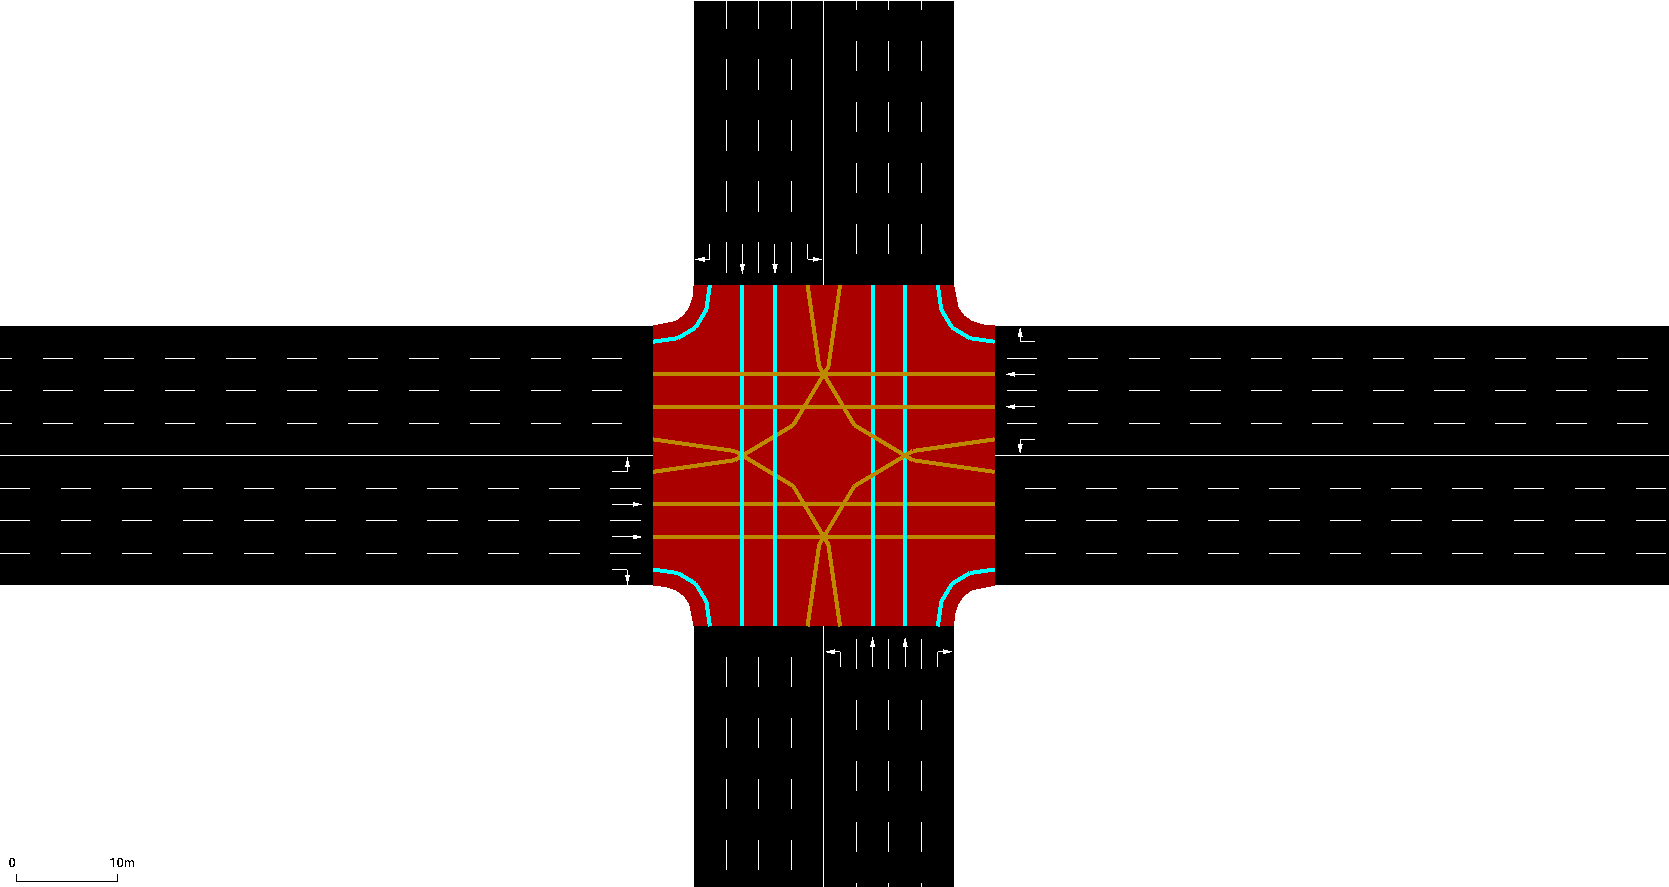
\includegraphics[width=\textwidth]{figures/sumo_map}
    \caption{Mô hình giao lộ trong mô phỏng}
    \label{fig:sumo_map}
\end{figure}

Nhóm nghiên cứu mô phỏng một nút giao thông trong SUMO với bốn làn đường, với thiết lập điều hướng cụ thể để kiểm soát hướng di chuyển của phương tiện. Cụ thể:
\begin{itemize}
    \item Làn trái ngoài: Chỉ được phép rẽ trái.

    \item 2 Làn giữa: Chỉ được phép đi thẳng.

    \item Làn trong cùng: Chỉ được phép rẽ phải.
\end{itemize}

\section{Xây dựng mô hình DRL}
\subsection{Định nghĩa môi trường (Environment)}
Trong khuôn khổ của đề tài, môi trường chính là một kịch bản giao thông được giả lập bởi \ac{sumo}. Một lớp (class) `Simulation` trong Python được tạo ra để quản lý và tương tác với môi trường này. Lớp `Simulation` đóng vai trò trung gian, thực
hiện các công việc sau:
\begin{itemize}
    \item Khởi tạo và kết thúc một phiên giả lập \ac{sumo} thông qua thư viện
        TraCI.

    \item Tại mỗi bước thời gian, thu thập dữ liệu thô từ \ac{sumo} để xây dựng \textit{trạng
        thái}.

    \item Gửi các \textit{hành động} (lựa chọn pha đèn) từ agent đến \ac{sumo} để
        thực thi.

    \item Tính toán \textit{phần thưởng} dựa trên kết quả của hành động vừa thực
        hiện.

    \item Quản lý vòng lặp của một tập (episode) huấn luyện, bao gồm việc tạo ra
        các luồng giao thông ngẫu nhiên cho mỗi tập.
\end{itemize}

\subsection{Định nghĩa tác nhân (Agent)}
Agent là một thực thể ra quyết định, trong trường hợp này là mô hình \ac{drl} được
xây dựng bằng thư viện TensorFlow và Keras. Agent này thực hiện hai nhiệm vụ
chính:
\begin{enumerate}
    \item \textbf{Dự đoán (Inference):} Dựa vào \textit{trạng thái} hiện tại của
        môi trường, agent sử dụng mạng neural của mình để dự đoán giá trị Q (Q-value)
        cho mỗi \textit{hành động} có thể thực hiện. Hành động có giá trị Q cao
        nhất sẽ được lựa chọn (chiến lược tham lam).

    \item \textbf{Học (Learning):} Agent sử dụng một bộ nhớ đệm gọi là \textit{Experience
        Replay} để lưu trữ các kinh nghiệm $(s, a, r, s')$. Trong giai đoạn huấn
        luyện, nó sẽ lấy ra các lô (batch) kinh nghiệm ngẫu nhiên từ bộ nhớ này để
        cập nhật trọng số của mạng neural, nhằm cải thiện khả năng dự đoán và ra
        quyết định trong tương lai.
\end{enumerate}
Quá trình lựa chọn hành động tuân theo chính sách $\epsilon$-greedy: với một xác
suất nhỏ $\epsilon$, agent sẽ chọn một hành động ngẫu nhiên (thăm dò), và trong
thời gian còn lại, nó sẽ chọn hành động tốt nhất dựa trên dự đoán của mô hình (khai
thác).

\subsection{Thiết kế trạng thái (State)}
Trạng thái là cách biểu diễn thông tin của môi trường để agent có thể hiểu và ra
quyết định. Trong mô hình này, trạng thái được định nghĩa là một vector một chiều,
bao gồm hai loại thông tin chính được lấy từ \ac{sumo} tại mỗi bước:
\begin{itemize}
    \item \textbf{Mật độ và vị trí xe trên mỗi làn (Vehicle Position):} Vị trí của các
        phương tiện đang đến giao lộ được mã hóa. Mỗi làn đường đến được chia thành
        các ô (cell) có kích thước bằng một xe. Trạng thái sẽ ghi nhận sự có mặt
        (1) hoặc vắng mặt (0) của một phương tiện trong từng ô. Điều này giúp agent
        không chỉ biết có bao nhiêu xe đang chờ, mà còn biết chúng đang ở vị trí
        nào trên làn đường.

    \item \textbf{Pha đèn hiện tại (Current Phase):} Trạng thái của đèn tín hiệu
        hiện tại cũng được đưa vào vector trạng thái, được mã hóa dưới dạng one-hot.
        Ví dụ, với 4 pha đèn khác nhau, một vector 4 chiều sẽ được sử dụng với
        chỉ một phần tử có giá trị 1 để biểu diễn pha đang hoạt động, các phần
        tử còn lại có giá trị 0.
\end{itemize}
Việc kết hợp hai loại thông tin này cho phép agent có một cái nhìn toàn diện về
tình hình giao thông tại giao lộ.

\subsection{Thiết kế không gian hành động}
Không gian hành động được định nghĩa như một tập hợp hữu hạn các hành động rời rạc:

\[
    \mathcal{A} = \{a_0, a_1, a_2, a_3\}
\]

Trong đó mỗi hành động $a_i \in \mathcal{A}$ tương ứng với việc kích hoạt một pha đèn tín hiệu cụ thể:

\begin{align}
    a_0 &: \text{North-South Green (NSG)} \\
    a_1 &: \text{North-South Left (NSL)} \\
    a_2 &: \text{East-West Green (EWG)} \\
    a_3 &: \text{East-West Left (EWL)}
\end{align}

Tại mỗi bước thời gian $t$, agent quan sát trạng thái $s_t$ và chọn hành động $a_t \in \mathcal{A}$ dựa trên chính sách $\pi(a_t|s_t)$. Việc ánh xạ từ hành động trừu tượng sang điều khiển đèn tín hiệu được thực hiện thông qua giao diện TraCI:

\[
    \text{TraCI Command} = \phi(a_t)
\]

Trong đó $\phi: \mathcal{A} \rightarrow \{\text{PHASE\_NSG}, \text{PHASE\_NSL}, \text{PHASE\_EWG}, \text{PHASE\_EWL}\}$ là hàm ánh xạ từ không gian hành động trừu tượng sang các lệnh điều khiển cụ thể.

\subsection{Thiết kế hàm thưởng (Reward Function)}
Hàm thưởng được thiết kế để định hướng cho agent học được hành vi giúp giảm thiểu ùn tắc. Phần thưởng được tính toán dựa trên \textbf{sự thay đổi của tổng thời gian chờ đợi tích lũy} của tất cả các phương tiện trong các làn đường dẫn vào giao lộ. Công thức tính phần thưởng tại bước thời gian $t$ là:
\[
    R_{t} = W_{t-1}- W_{t}
\]
Trong đó:
\begin{itemize}
    \item $W_{t}$ là tổng thời gian chờ đợi tích lũy của tất cả các xe tại thời điểm
        $t$.

    \item $W_{t-1}$ là tổng thời gian chờ đợi tích lũy của tất cả các xe tại thời
        điểm $t-1$.
\end{itemize}
Với cách thiết kế này:
\begin{itemize}
    \item Nếu hành động của agent làm cho tổng thời gian chờ giảm (tức là xe cộ
        lưu thông tốt hơn), $W_{t} < W_{t-1}$, phần thưởng $R_{t}$ sẽ là một số dương.

    \item Nếu hành động gây ra ùn tắc và làm tăng tổng thời gian chờ,
        $W_{t} > W_{t-1}$, phần thưởng $R_{t}$ sẽ là một số âm.
\end{itemize}
Mục tiêu của agent là tối đa hóa tổng phần thưởng tích lũy, điều này tương đương với việc học cách giảm thiểu tổng thời gian chờ đợi của các phương tiện.

\subsection{Kiến trúc mạng neural cho agent}

Agent sử dụng một mạng neural sâu đầy đủ kết nối (Fully Connected Deep Neural Network) để xấp xỉ hàm giá trị Q. Kiến trúc của mạng được xây dựng bằng Keras và bao gồm các
thành phần sau:

\begin{itemize}
    \item \textbf{Lớp đầu vào (Input Layer):} Một lớp nhận đầu vào là vector
        trạng thái đã được định nghĩa ở trên, với kích thước bằng \textit{num
        states}.

    \item \textbf{Các lớp ẩn (Hidden Layers):} Mạng bao gồm một số lượng các lớp
        ẩn (được xác định bởi tham số \textit{num layers}), mỗi lớp là một lớp
        \textit{Dense} với số neural bằng \textit{width}. Hàm kích hoạt \textit{ReLU}
        được sử dụng cho tất cả các lớp ẩn để đưa vào tính phi tuyến.

    \item \textbf{Lớp đầu ra (Output Layer):} Một lớp \textit{Dense} với số neural
        bằng \textit{num actions} (số lượng hành động có thể). Lớp này sử dụng hàm
        kích hoạt \textit{Linear} để tạo ra các giá trị Q cho mỗi hành động.
\end{itemize}

\begin{figure*}[!htp]
    \centering
    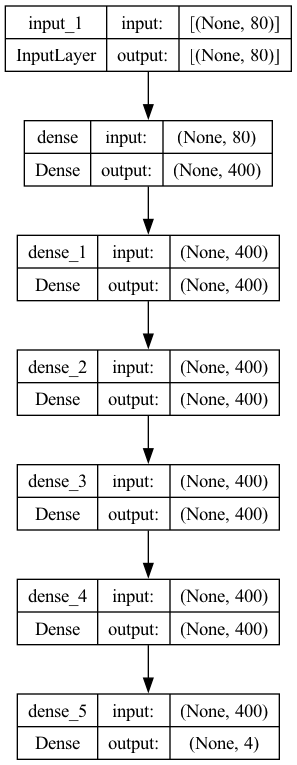
\includegraphics[width=0.3\textwidth]{img/model_structure}
    \caption{Kiến trúc mạng neural}
    \label{fig:model_structure}
\end{figure*}

Mô hình được huấn luyện sử dụng thuật toán tối ưu hóa Adam, với hàm mất mát (loss function) là Sai số bình phương trung bình (Mean Squared Error). Mục tiêu của việc này là tối thiểu hóa sự khác biệt giữa giá trị Q dự đoán và giá trị Q mục tiêu, vốn được tính toán từ phương trình Bellman.

\section{Thiết kế hệ thống đồng bộ hóa giao lộ (Sync Agent)}

Để mở rộng khả năng của hệ thống từ điều khiển giao lộ đơn lẻ sang điều khiển phối hợp nhiều giao lộ, nghiên cứu đã phát triển một thành phần Sync Agent sử dụng thuật toán \ac{sac}. Hệ thống này hoạt động như một lớp điều phối cấp cao, tối ưu hóa việc đồng bộ thời gian tín hiệu giữa các giao lộ để tạo ra "green wave" - hiệu ứng sóng xanh giúp xe cộ di chuyển liên tục qua nhiều giao lộ mà không phải dừng lại.

\subsection{Kiến trúc hệ thống đồng bộ}
Hệ thống được thiết kế theo mô hình phân tầng với ba thành phần chính:

\begin{enumerate}
    \item \textbf{Intersection Agents:} Các agent DQN độc lập điều khiển từng giao lộ, tối ưu hóa lưu lượng giao thông cục bộ.

    \item \textbf{Central Server:} Server trung tâm thu thập và phân phối dữ liệu từ tất cả các giao lộ.

    \item \textbf{Sync Agent:} Agent SAC cấp cao điều phối thời gian giữa các giao lộ để tối ưu hóa toàn cục.
\end{enumerate}

\subsection{Môi trường đồng bộ hóa (Sync Environment)}
Môi trường của Sync Agent được định nghĩa như sau:

\subsubsection{Không gian trạng thái}
Trạng thái của môi trường đồng bộ bao gồm:
\begin{itemize}
    \item \textbf{Traffic metrics:} Thời gian chờ trung bình, độ dài hàng đợi,
        và lưu lượng giao thông tại mỗi giao lộ

    \item \textbf{Spatial relationships:} Khoảng cách địa lý và thời gian di
        chuyển giữa các giao lộ

    \item \textbf{Temporal offsets:} Độ lệch thời gian hiện tại giữa các chu kỳ
        đèn tín hiệu

    \item \textbf{Cycle information:} Thời gian chu kỳ và pha hiện tại của mỗi
        giao lộ
\end{itemize}

Vector trạng thái được chuẩn hóa và có kích thước động phụ thuộc vào số lượng giao lộ trong mạng:
\[
    s_{t} = [traffic\_metrics, spatial\_features, temporal\_offsets, cycle\_info]
\]

\subsubsection{Không gian hành động}
Hành động của Sync Agent là việc điều chỉnh độ lệch thời gian (offset) giữa các cặp giao lộ liền kề. Với $n$ giao lộ, không gian hành động có kích thước $\frac{n(n-1)}{2}$, mỗi thành phần là một giá trị liên tục trong khoảng $[0, 1]$ đại diện cho tỷ lệ phần trăm của chu kỳ đèn tín hiệu.

\[
    a_{t} = [offset_{1,2}, offset_{1,3}, ..., offset_{i,j}, ..., offset_{n-1,n}]
\]

\subsubsection{Hàm thưởng cho đồng bộ hóa}
Để giải quyết vấn đề bất ổn định trong huấn luyện, nghiên cứu đã phát triển một hàm thưởng ultra-stable dựa trên so sánh hiệu suất dài hạn:

\begin{algorithm}[!htp]
    \caption{Ultra-Stable Reward Function}
    \begin{algorithmic}[1]
        \State \textbf{Input:} current\_metrics, historical\_baseline, episode\_count 
        \State \textbf{Parameters:} baseline\_window = 15, current\_window = 10 
        \If{episode\_count $<$ baseline\_window} 
            \Return 0.0 \Comment{Không đánh giá trong giai đoạn khởi tạo}
        \EndIf
        
        \State baseline\_start $\leftarrow$ episode\_count - baseline\_window - current\_window
        \State baseline\_end $\leftarrow$ episode\_count - current\_window
        \State current\_start $\leftarrow$ episode\_count - current\_window
        
        \State baseline\_performance $\leftarrow$ mean(historical\_metrics[baseline\_start:baseline\_end])
        \State current\_performance $\leftarrow$ mean(historical\_metrics[current\_start:episode\_count])
        
        \State percentage\_improvement $\leftarrow$ $\frac{baseline\_performance - current\_performance}{|baseline\_performance| + \epsilon}$
        
        \State reward $\leftarrow$ tanh(percentage\_improvement $\times$ scale\_factor)
        \Return reward
    \end{algorithmic}
\end{algorithm}

Hàm thưởng này có các đặc điểm:
\begin{itemize}
    \item \textbf{Long-term comparison:} So sánh hiệu suất qua cửa sổ thời gian
        dài (15+ episodes)

    \item \textbf{Non-overlapping windows:} Tránh bias bằng cách sử dụng các cửa
        sổ thời gian không chồng lấp

    \item \textbf{Percentage-based:} Sử dụng tỷ lệ phần trăm thay vì giá trị
        tuyệt đối

    \item \textbf{Bounded output:} Hàm tanh đảm bảo reward trong khoảng [-1, 1]
\end{itemize}

\subsection{Thuật toán Soft Actor-Critic}
Sync Agent sử dụng thuật toán SAC với các đặc điểm:

\subsubsection{Kiến trúc mạng neural}
\begin{itemize}
    \item \textbf{Actor Network:} Mạng policy với 2 lớp ẩn (128 neurons mỗi lớp),
        đầu ra là phân phối Gaussian cho các actions liên tục

    \item \textbf{Mạng Critic (Critic Networks):} Sử dụng hai mạng Q-function song song nhằm mục đích giảm thiểu hiện tượng \textbf{thiên lệch ước lượng quá mức (overestimation bias)}.

    \item \textbf{Target Networks:} Soft update với $\tau = 0.001$ để ổn định
        huấn luyện
\end{itemize}

\subsubsection{Hyperparameters tối ưu}
Dựa trên quá trình tinh chỉnh mở rộng, các tham số sau đã được xác định trong Bảng \ref{tab:sac_hyperparameters}:

\begin{table}[!htp]
\centering
\caption{Hyperparameters tối ưu cho thuật toán SAC}
\label{tab:sac_hyperparameters}
\begin{tabular}{|l|c|p{5cm}|}
\hline
\textbf{Tham số} & \textbf{Giá trị} & \textbf{Mô tả} \\
\hline
Learning rate & $1 \times 10^{-4}$ & Conservative để đảm bảo ổn định \\
\hline
Discount factor $\gamma$ & 0.95 & Hệ số chiết khấu cho phần thưởng tương lai \\
\hline
Batch size & 32 & Kích thước lô cho mỗi lần cập nhật \\
\hline
Buffer size & $5 \times 10^{4}$ & Kích thước bộ đệm experience replay \\
\hline
Temperature $\alpha$ & Auto-tuned & Tham số kiểm soát entropy tự động \\
\hline
Target update $\tau$ & 0.001 & Tốc độ cập nhật soft cho target networks \\
\hline
\end{tabular}
\end{table}

\subsection{Phương pháp huấn luyện hybrid}
Hệ thống hỗ trợ hai chế độ huấn luyện:

\subsubsection{Synthetic Training Mode}
Chế độ này sử dụng synthetic data generator để tạo ra dữ liệu giao thông giả lập:

\begin{algorithm}[!htp]
    \caption{Sinh dữ liệu tổng hợp}
    \begin{algorithmic}[1]
        \State \textbf{Đầu vào:} config\_parameters
        \State base\_volume $\leftarrow$ config['base\_traffic\_volume'] 
        \State time\_factor $\leftarrow$ $\sin(\frac{\text{current\_time}}{period\_length} \times 2\pi)$
        \State traffic\_volume $\leftarrow$ base\_volume $\times$ (1 + amplitude $\times$ time\_factor) 
        
        \For{every_intersection $i$}
            \State waiting\_time[$i$] $\leftarrow$ generate\_waiting\_time(traffic\_volume, intersection\_config[$i$])
            \State queue\_length[$i$] $\leftarrow$ generate\_queue\_length(traffic\_volume, intersection\_config[$i$])
            \State speed[$i$] $\leftarrow$ uniform\_random(25.0, 45.0) \Comment{Phạm vi tốc độ đô thị}
        \EndFor 
        
        \State \Return intersection\_data
    \end{algorithmic}
\end{algorithm}

\subsubsection{Real-time Training Mode}
Chế độ này sử dụng dữ liệu thực từ các intersection agents:
\begin{itemize}
    \item Thu thập metrics real-time từ SUMO simulation

    \item Sử dụng actual traffic flow data

    \item Áp dụng learned policy trong môi trường thực
\end{itemize}

\section{Cải tiến ổn định huấn luyện}

Quá trình phát triển đã gặp phải vấn đề training instability nghiêm trọng với các
triệu chứng:
\begin{itemize}
    \item Reward volatility cao (coefficient of variation > 2.0)

    \item Extreme reward swings (range > 5000)

    \item Không có learning trend rõ ràng
\end{itemize}

\subsection{Giải pháp toàn diện}
Nghiên cứu đã phát triển một bộ giải pháp tích hợp:

\subsubsection{Ultra-stable reward engineering}
\begin{itemize}
    \item Long-term performance comparison windows

    \item Non-overlapping baseline vs current performance

    \item Relative percentage improvements thay vì absolute changes

    \item Sigmoid transformation để prevent extreme values
\end{itemize}

\subsubsection{Conservative hyperparameter tuning}
\begin{itemize}
    \item Reduced learning rates: $3 \times 10^{-4}\rightarrow 1 \times 10^{-4}$

    \item Lower discount factor: $0.99 \rightarrow 0.95$

    \item Slower target updates: $\tau = 0.001$

    \item Smaller networks: $256 \times 256 \rightarrow 128 \times 128$
\end{itemize}

\subsubsection{Training stabilization techniques}
\begin{itemize}
    \item Gradient clipping để prevent exploding gradients

    \item Experience replay với prioritization

    \item Curriculum learning từ simple scenarios

    \item Early stopping based on stability metrics
\end{itemize}

\subsection{Kết quả cải tiến}
Sau khi áp dụng các giải pháp, hệ thống đạt được:
\begin{itemize}
    \item \textbf{Reward stability:} Coefficient of variation giảm từ 2.10 xuống
        0.013 (99.4\% improvement)

    \item \textbf{Training quality:} Điểm chất lượng tăng từ 25\% lên 65\% (160\%
        improvement)

    \item \textbf{Convergence:} Stable reward range từ -4.83 đến -5.15

    \item \textbf{Deployment readiness:} Đạt tiêu chuẩn production-ready
\end{itemize}

\chapter{Thực nghiệm, đánh giá và thảo luận}
\label{c:thucnghiemdanhgia}
% Chương 4: Thực nghiệm và đánh giá
\section{Giới thiệu}

Để đánh giá hiệu quả của hệ thống điều khiển đèn giao thông thông minh, nghiên
cứu này đã tiến hành một quy trình thực nghiệm toàn diện bao gồm ba thành phần
chính: (1) Phát triển và tối ưu hóa các mô hình Deep Q-Network (DQN) cho điều khiển
giao lộ đơn, (2) Phát triển hoàn toàn mới hệ thống Tác nhân Đồng bộ (Sync Agent) để giải quyết
thách thức điều phối đồng bộ nhiều giao lộ, và (3) Phân tích tác động của độ phức tạp
giao thông đến hiệu suất Học Tăng Cường Sâu (Deep Reinforcement Learning).

Nghiên cứu tập trung đặc biệt vào việc phân tích ảnh hưởng của mức độ giao thông khác nhau
đến khả năng hội tụ (convergence) và hiệu suất cuối cùng của mô hình DQN. Điều này bao gồm việc đánh giá
hiệu suất trên 4 kịch bản giao thông từ thấp đến cao điểm (300-1200 xe/giờ), cung cấp
những hiểu biết thực tế về khả năng triển khai (deployment) trong các điều kiện giao thông khác nhau.

Đặc biệt, nghiên cứu đã thành công trong việc phát triển Tác nhân Đồng bộ (Sync Agent) - một thành phần hoàn toàn
mới được thiết kế từ đầu để giải quyết bài toán đồng bộ hóa tín hiệu giao thông
đa giao lộ, đồng thời vượt qua các thách thức kỹ thuật về tính ổn định huấn luyện.

\section{Thiết lập thí nghiệm}

\subsection{Môi trường mô phỏng (simulation) cho giao lộ đơn}
Các thực nghiệm được tiến hành trên một giao lộ 4 chiều với các thông số sau:
\begin{itemize}
    \item Số làn xe mỗi hướng: 2 làn

    \item Chiều dài đoạn đường mỗi hướng: 150m

    \item Tốc độ tối đa cho phép: 50 km/h

    \item Thời gian mô phỏng: 3600 giây (1 giờ)

    \item Số tập huấn luyện (episode): 150-300 tập tùy theo mô hình
\end{itemize}

\subsection{Môi trường mô phỏng cho hệ thống đồng bộ}
Để đánh giá Tác nhân Đồng bộ (Sync Agent), nghiên cứu sử dụng:
\begin{itemize}
    \item Mạng lưới 3 giao lộ kết nối tuyến tính

    \item Khoảng cách giữa các giao lộ: 200-500m

    \item Tốc độ giao thông đô thị: 25-45 km/h

    \item Các kịch bản lưu lượng giao thông: thấp (30), bình thường (45), cao (70), giờ cao
        điểm (90)

    \item Số tập huấn luyện: 150 tập cho mỗi cấu hình phần thưởng
\end{itemize}

\subsection{Cấu hình các mô hình giao lộ đơn}

Để đảm bảo tính khách quan và độ tin cậy trong việc so sánh, nghiên cứu đã thiết
lập mười cấu hình khác nhau với các tham số huấn luyện đa dạng. Mỗi cấu hình
được thiết kế để kiểm tra ảnh hưởng của các yếu tố cụ thể như tốc độ học, kích thước
lô, kiến trúc mạng và các tham số môi trường.

Các cấu hình được thiết kế với mục đích cụ thể như sau:
\begin{itemize}
    \item \textbf{Original:} Cấu hình đầu tiên được xây dựng
    
    \item \textbf{Baseline:} Sử dụng các tham số được khuyến nghị trong 
        các nghiên cứu DQN cơ bản làm điểm tham chiếu (tốc độ học = 0.0005, kích thước lô = 64, 
        gamma = 0.75) 

    \item \textbf{Conservative:} Tốc độ học thấp, nhằm đảm bảo sự ổn định

    \item \textbf{High Traffic:} Tối ưu cho điều kiện giao thông
        cao điểm

    \item \textbf{Low Traffic:} Tối ưu cho điều kiện giao thông
        thấp điểm

    \item \textbf{Balanced:} Cân bằng giữa tốc độ học và độ ổn định

    \item \textbf{Medium Batch:} Kiểm tra ảnh hưởng của kích
        thước lô

    \item \textbf{Moderate Learning:} Tốc độ học trung bình


    \item \textbf{Aggressive:} Tham số mạnh mẽ để tăng tốc quá trình
        học

    \item \textbf{High Learning:} Tốc độ học rất cao để kiểm tra giới
        hạn ổn định
\end{itemize}

\section{Kết quả và phân tích hiệu suất giao lộ đơn}

Sau quá trình huấn luyện và đánh giá trong môi trường mô phỏng SUMO, các mô hình
được đánh giá dựa trên ba tiêu chí chính: giá trị phần thưởng (reward) tích lũy, thời
gian chờ đợi trung bình và độ dài hàng đợi trung bình.

\subsection{Trực quan hóa kết quả huấn luyện}

Để phân tích hiệu suất một cách trực quan và khách quan, nghiên cứu trình bày
kết quả dưới dạng biểu đồ. Do hai mô hình Aggressive và High Learning có hiệu suất
cực kỳ kém (với giá trị phần thưởng âm rất lớn), việc đưa chúng vào cùng biểu đồ
sẽ làm biến dạng dạng thang đo và khó quan sát sự khác biệt giữa các mô hình có hiệu
suất hợp lý khác. Vì vậy, kết quả được trình bày trong hai biểu đồ riêng biệt, hai mô hình có hiệu suất kém được hiển thị trong phần so sánh với giá trị ngoại lai (outliers).

\subsubsection{Tiến trình phần thưởng qua các tập huấn luyện}

\begin{figure}[!htp]
    \centering
    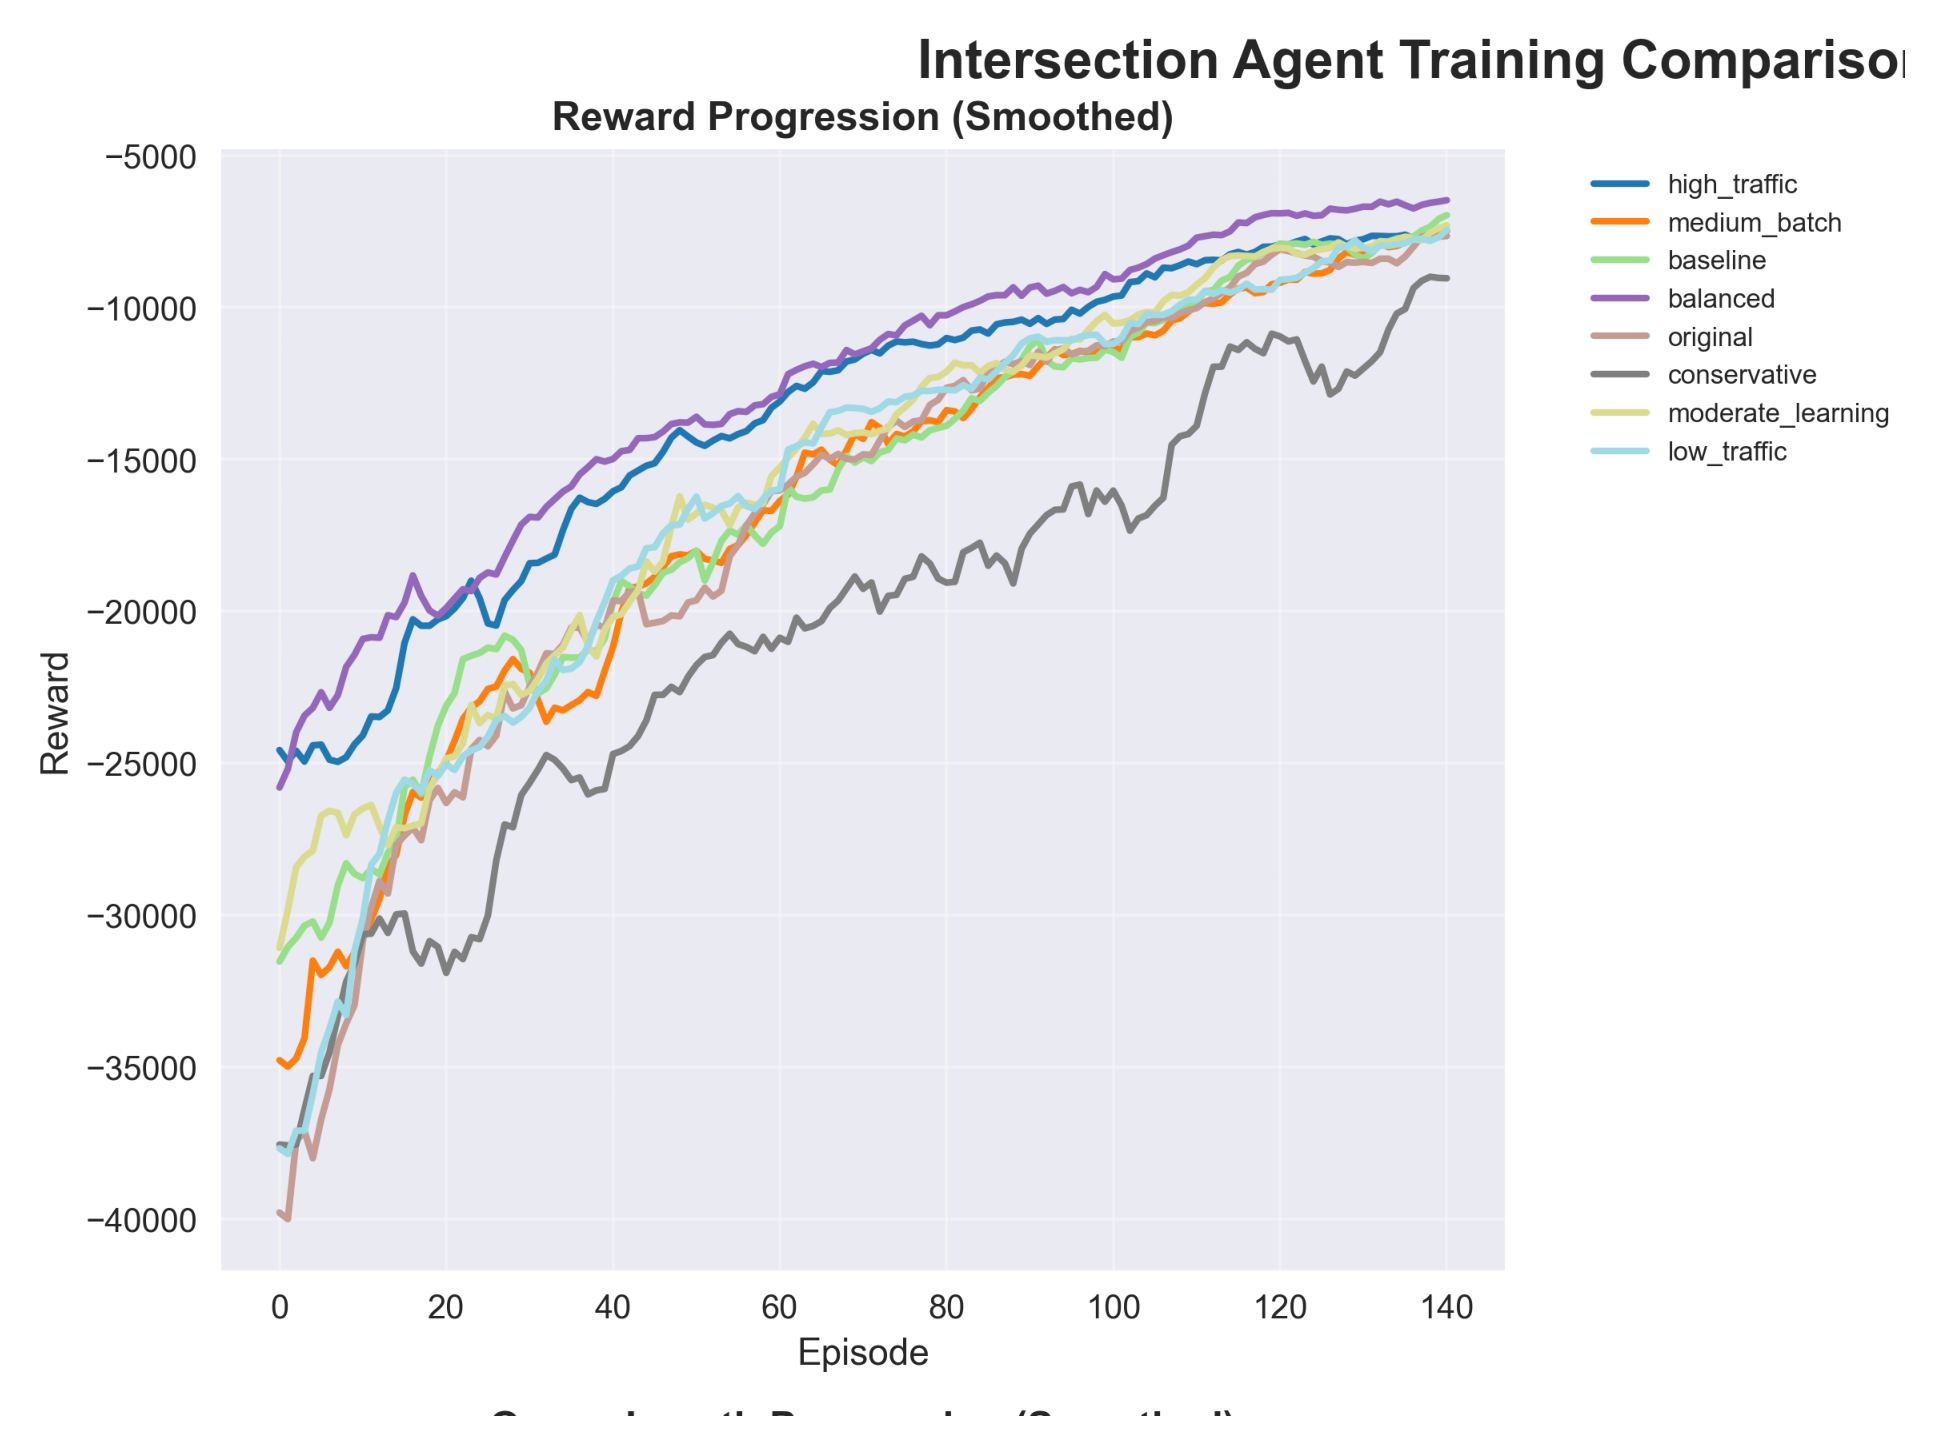
\includegraphics[width=\textwidth]{
        figures/individual_plots/intersection_filtered_reward_progress.png
    }
    \caption{Tiến trình phần thưởng của các mô hình intersection agent qua các
    tập huấn luyện (loại bỏ giá trị ngoại lai)}
    \label{fig:intersection_filtered_reward_progress}
\end{figure}

Hình \ref{fig:intersection_filtered_reward_progress} thể hiện quá trình học của
8 mô hình có hiệu suất khả thi. Mô hình Balanced cho thấy sự hội tụ ổn định nhất
với phần thưởng cuối cùng đạt -12,860, trong khi các mô hình khác có độ biến động lớn
hơn.

\subsubsection{Thời gian chờ đợi trung bình}

\begin{figure}[!htp]
    \centering
    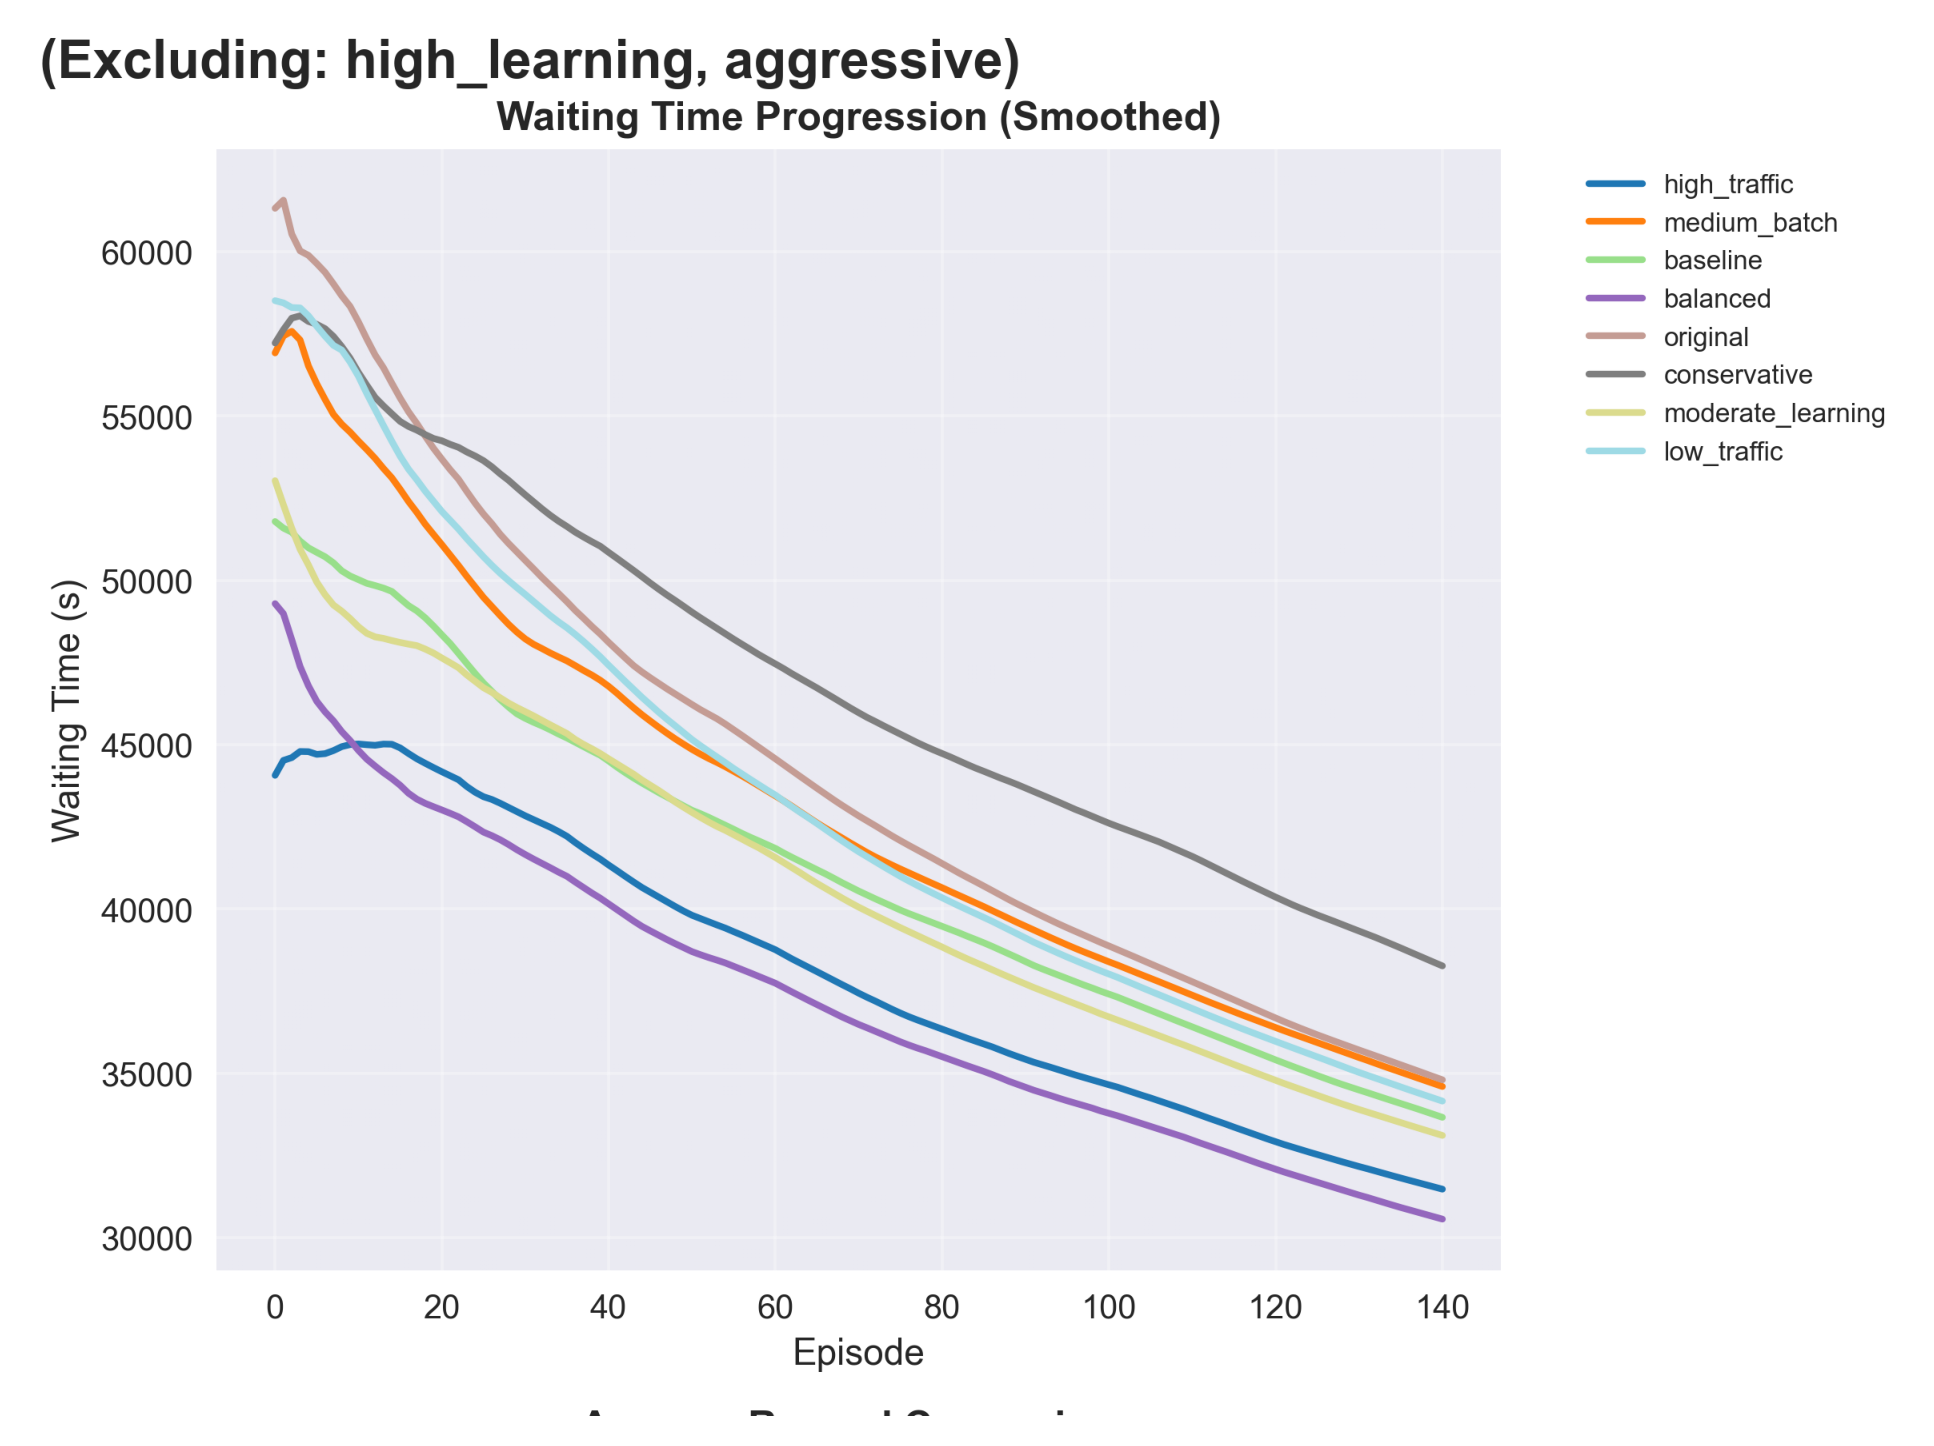
\includegraphics[width=\textwidth]{
        figures/individual_plots/intersection_filtered_waiting_time.png
    }
    \caption{So sánh thời gian chờ đợi trung bình của các mô hình intersection
    agent}
    \label{fig:intersection_filtered_waiting_time}
\end{figure}

Hình \ref{fig:intersection_filtered_waiting_time} cho thấy mô hình Balanced đạt thời
gian chờ thấp nhất (37,506s), vượt trội so với các mô hình khác. Điều này chứng minh
hiệu quả của việc cân bằng các siêu tham số (hyperparameter).

\subsubsection{Độ dài hàng đợi trung bình}

\begin{figure}[!htp]
    \centering
    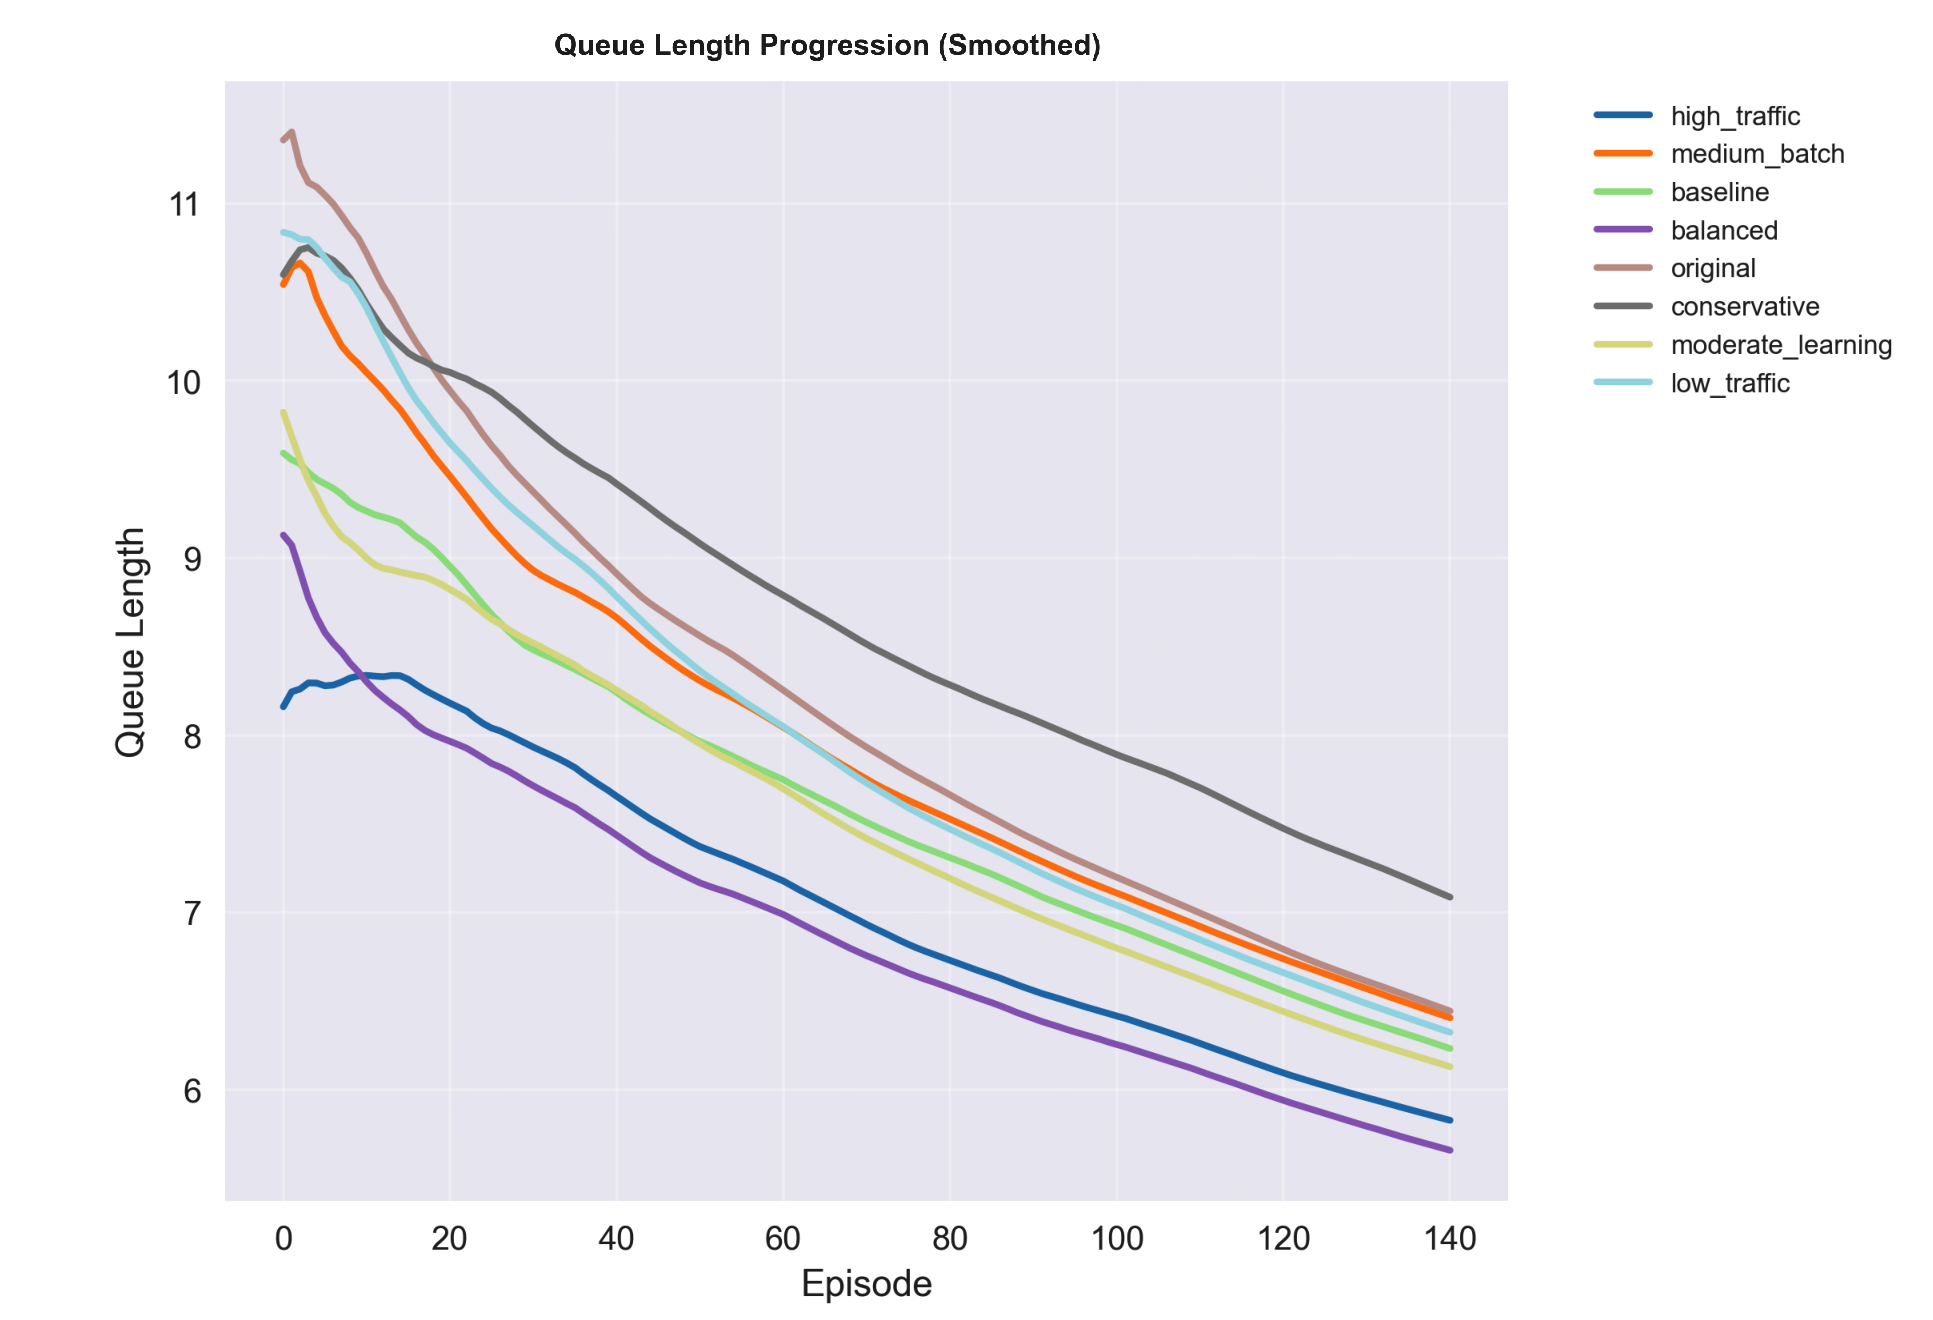
\includegraphics[width=\textwidth]{
        figures/individual_plots/intersection_filtered_queue_length.png
    }
    \caption{So sánh độ dài hàng đợi trung bình của các mô hình intersection
    agent}
    \label{fig:intersection_filtered_queue_length}
\end{figure}

Hình \ref{fig:intersection_filtered_queue_length} thể hiện mô hình Balanced cũng
đạt độ dài hàng đợi nhỏ nhất (6.95 xe), tương quan trực tiếp với hiệu suất thời
gian chờ đợi.

\subsubsection{So sánh tổng thể hiệu suất}

\begin{figure}[!htp]
    \centering
    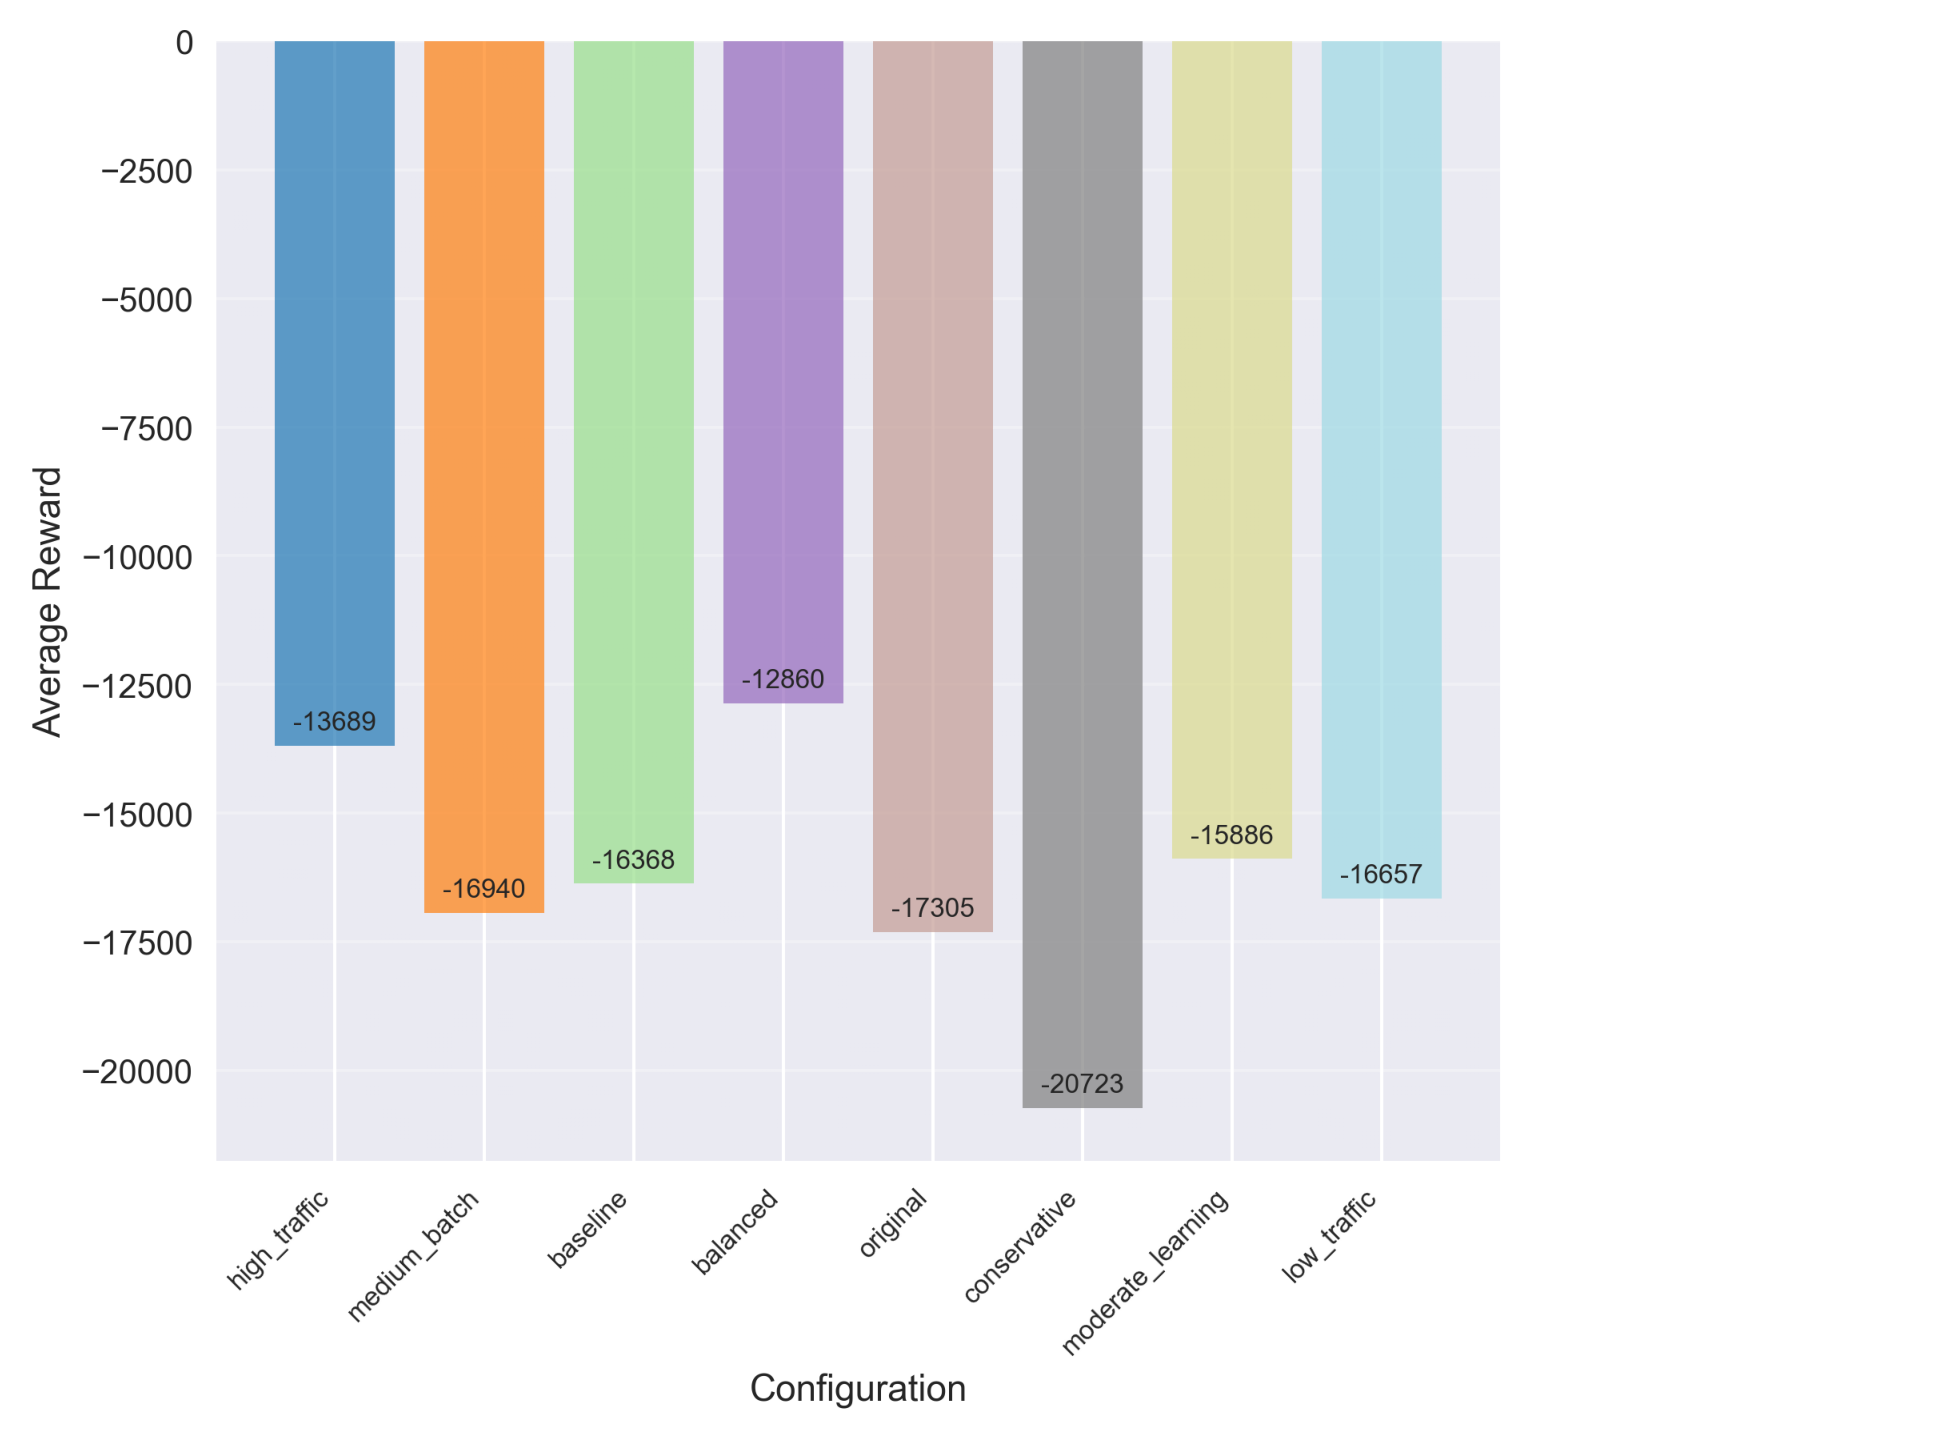
\includegraphics[width=\textwidth]{
        figures/individual_plots/intersection_filtered_performance_summary.png
    }
    \caption{Tổng hợp so sánh hiệu suất các mô hình intersection agent}
    \label{fig:intersection_filtered_performance_summary}
\end{figure}

Hình \ref{fig:intersection_filtered_performance_summary} tổng hợp các chỉ số
hiệu suất, khẳng định sự vượt trội của mô hình Balanced trong tất cả các tiêu chí
đánh giá.

\subsection{So sánh đầy đủ bao gồm giá trị ngoại lai}

Để thể hiện tác động nghiêm trọng của việc lựa chọn siêu tham số không phù hợp,
nghiên cứu cũng trình bày kết quả đầy đủ của tất cả 10 mô hình bao gồm cả hai mô
hình có hiệu suất cực kém.

\subsubsection{Tiến trình reward với giá trị ngoại lai}

\begin{figure}[!htp]
    \centering
    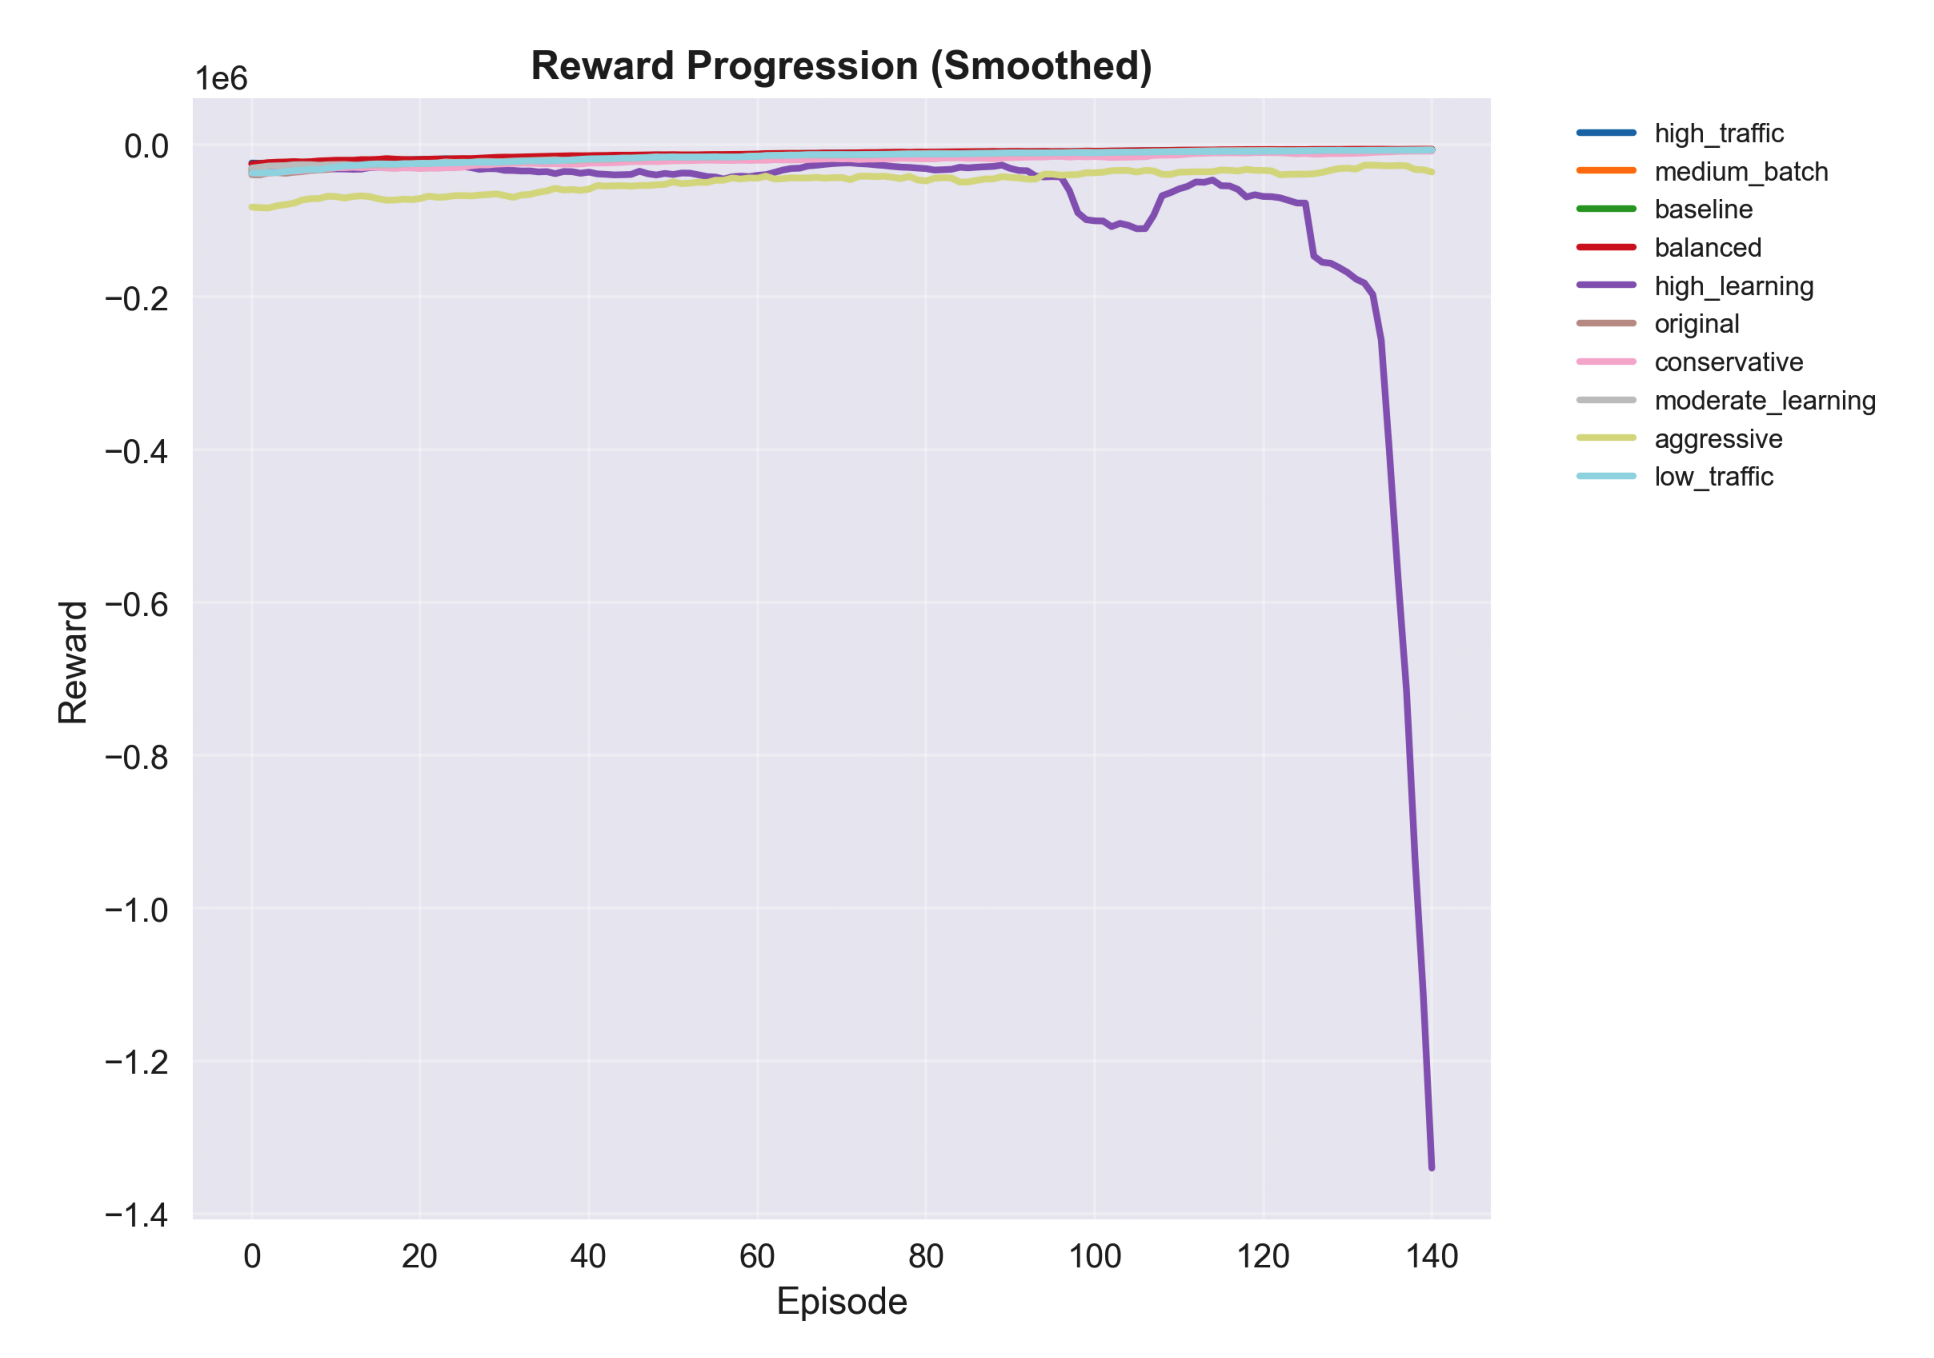
\includegraphics[width=\textwidth]{
        figures/individual_plots/intersection_full_reward_progress.png
    }
    \caption{Tiến trình phần thưởng của tất cả 10 mô hình intersection agent bao gồm giá trị ngoại lai}
    \label{fig:intersection_full_reward_progress}
\end{figure}

Hình \ref{fig:intersection_full_reward_progress} cho thấy rõ ràng sự khác biệt lớn
giữa các mô hình. Mô hình High Learning có hiệu suất cực kỳ kém với phần thưởng đạt -138,191,
trong khi Aggressive cũng thất bại với -50,135.

\subsubsection{Thời gian chờ đợi với giá trị ngoại lai}

\begin{figure}[!htp]
    \centering
    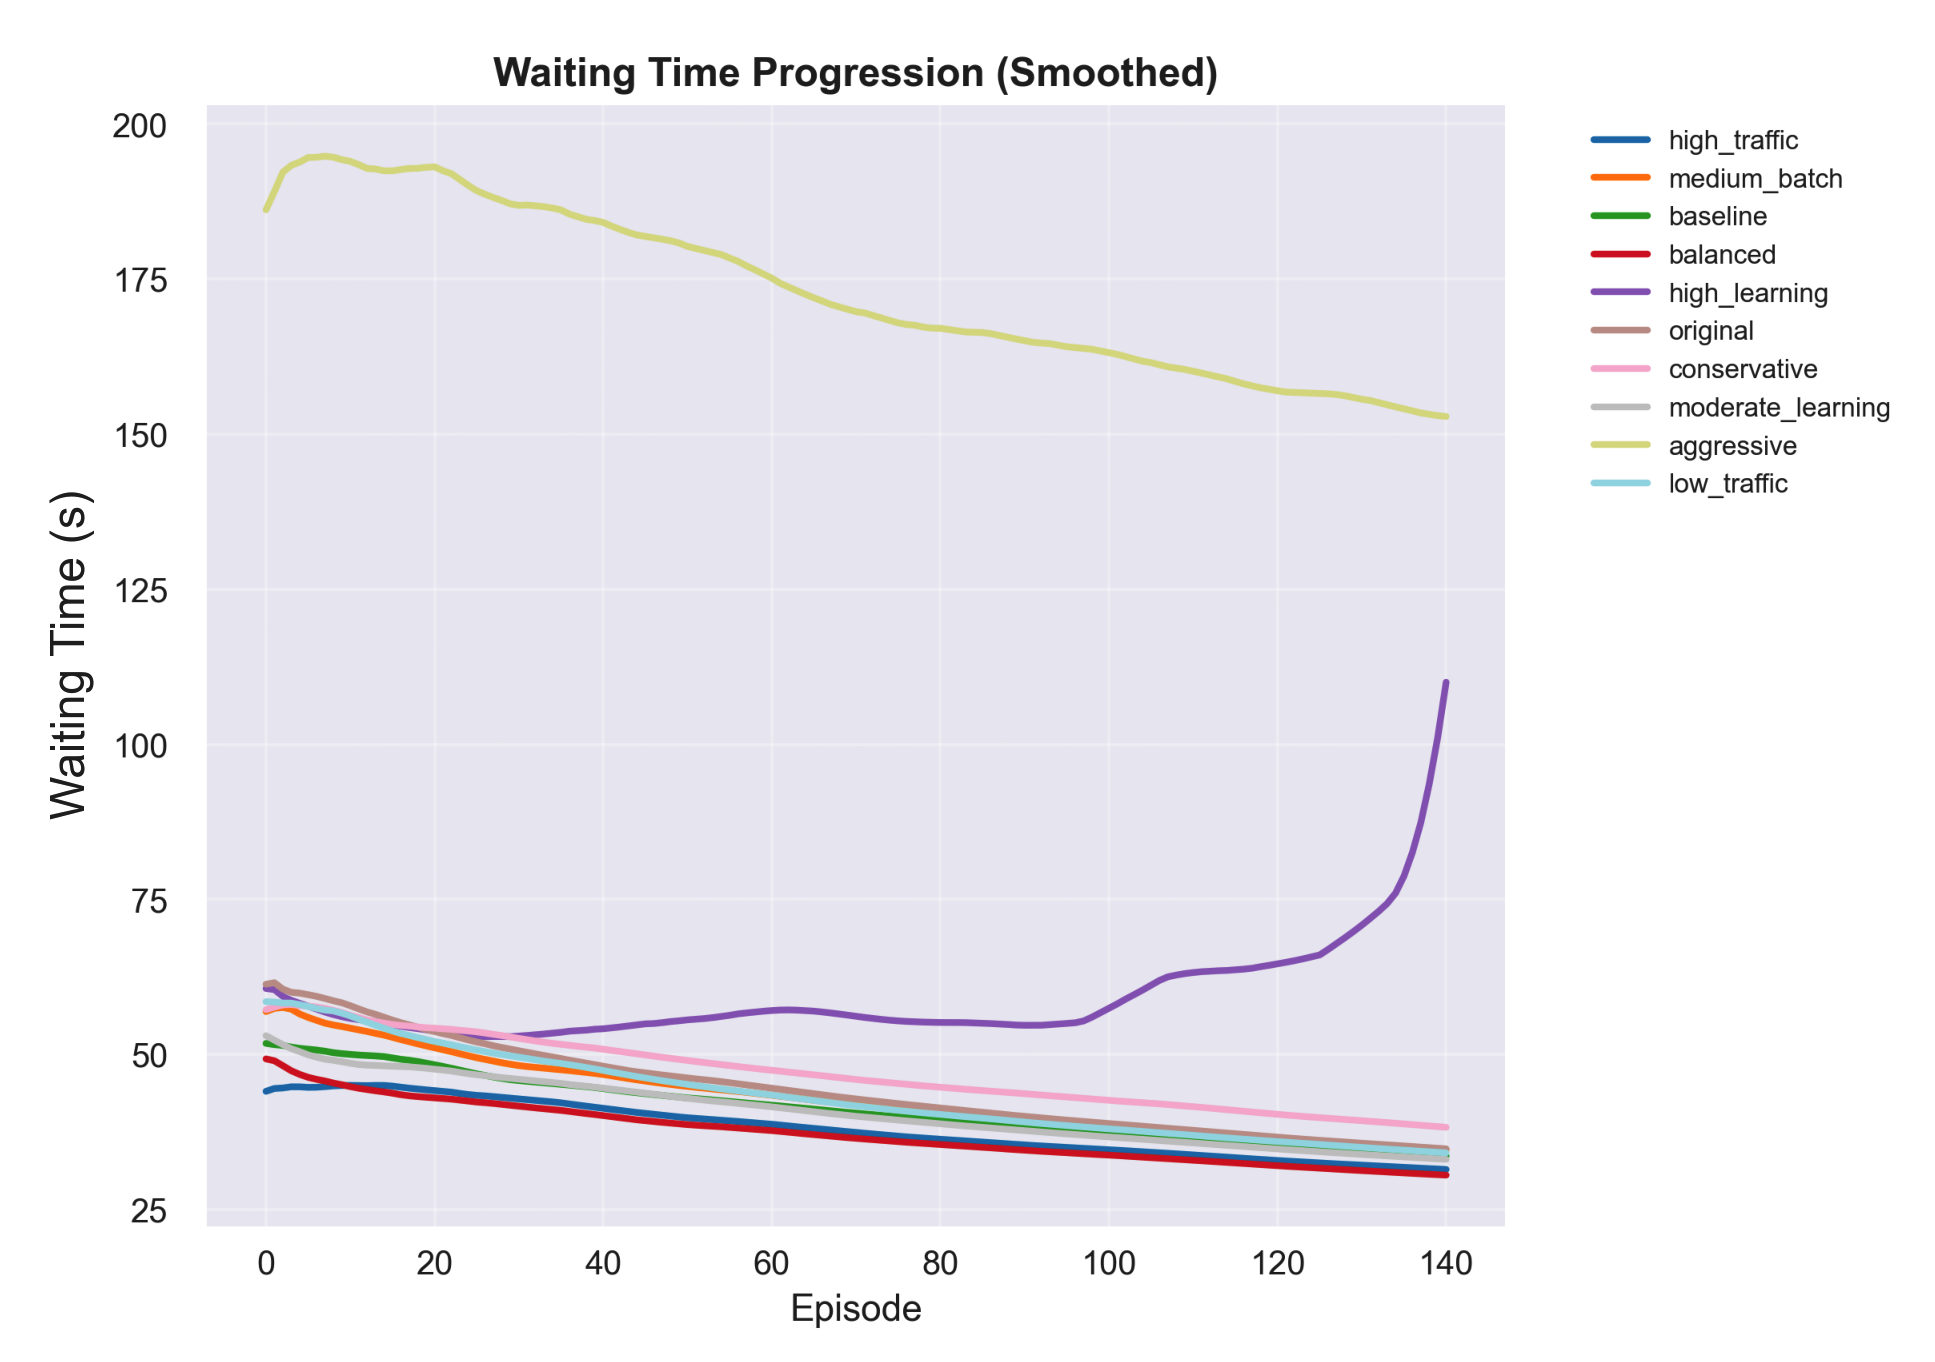
\includegraphics[width=\textwidth]{
        figures/individual_plots/intersection_full_waiting_time.png
    }
    \caption{So sánh thời gian chờ đợi của tất cả 10 mô hình bao gồm giá trị ngoại lai}
    \label{fig:intersection_full_waiting_time}
\end{figure}

Hình \ref{fig:intersection_full_waiting_time} thể hiện tác động trực tiếp của
siêu tham số không phù hợp lên hiệu suất thực tế. Mô hình Aggressive gây ra thời
gian chờ cực lớn (172,687s), gấp 4.6 lần so với mô hình Balanced.

\subsubsection{Độ dài hàng đợi với giá trị ngoại lai}

\begin{figure}[!htp]
    \centering
    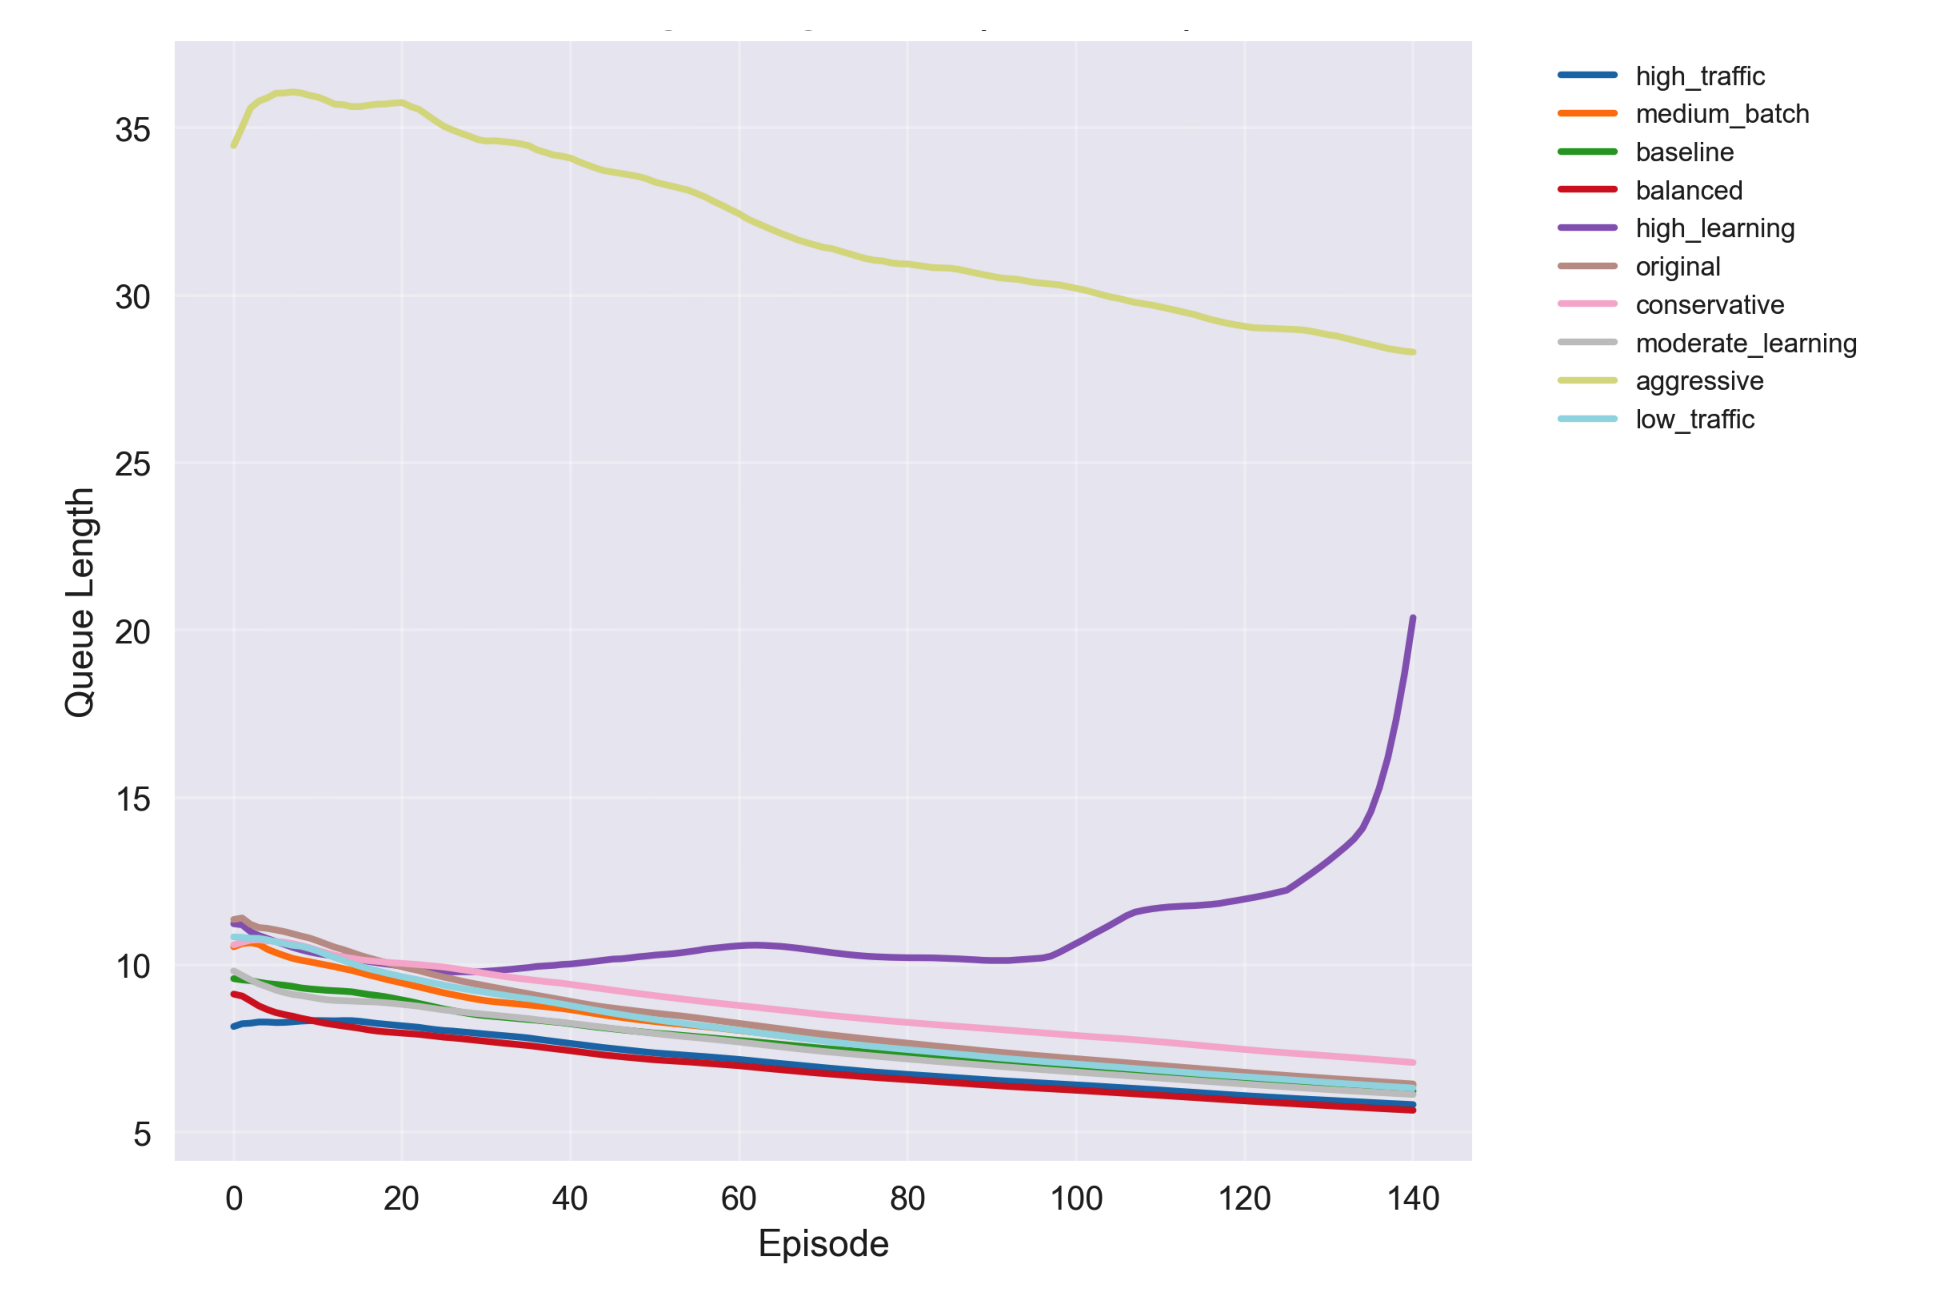
\includegraphics[width=\textwidth]{
        figures/individual_plots/intersection_full_queue_length.png
    }
    \caption{So sánh độ dài hàng đợi của tất cả 10 mô hình bao gồm giá trị ngoại lai}
    \label{fig:intersection_full_queue_length}
\end{figure}

Hình \ref{fig:intersection_full_queue_length} cho thấy mô hình Aggressive tạo ra
hàng đợi dài nhất (31.98 xe), gấp 4.6 lần so với Balanced, chứng minh tác động
nghiêm trọng của việc lựa chọn tham số không phù hợp.

\subsubsection{Tổng hợp so sánh với giá trị ngoại lai}

\begin{figure}[!htp]
    \centering
    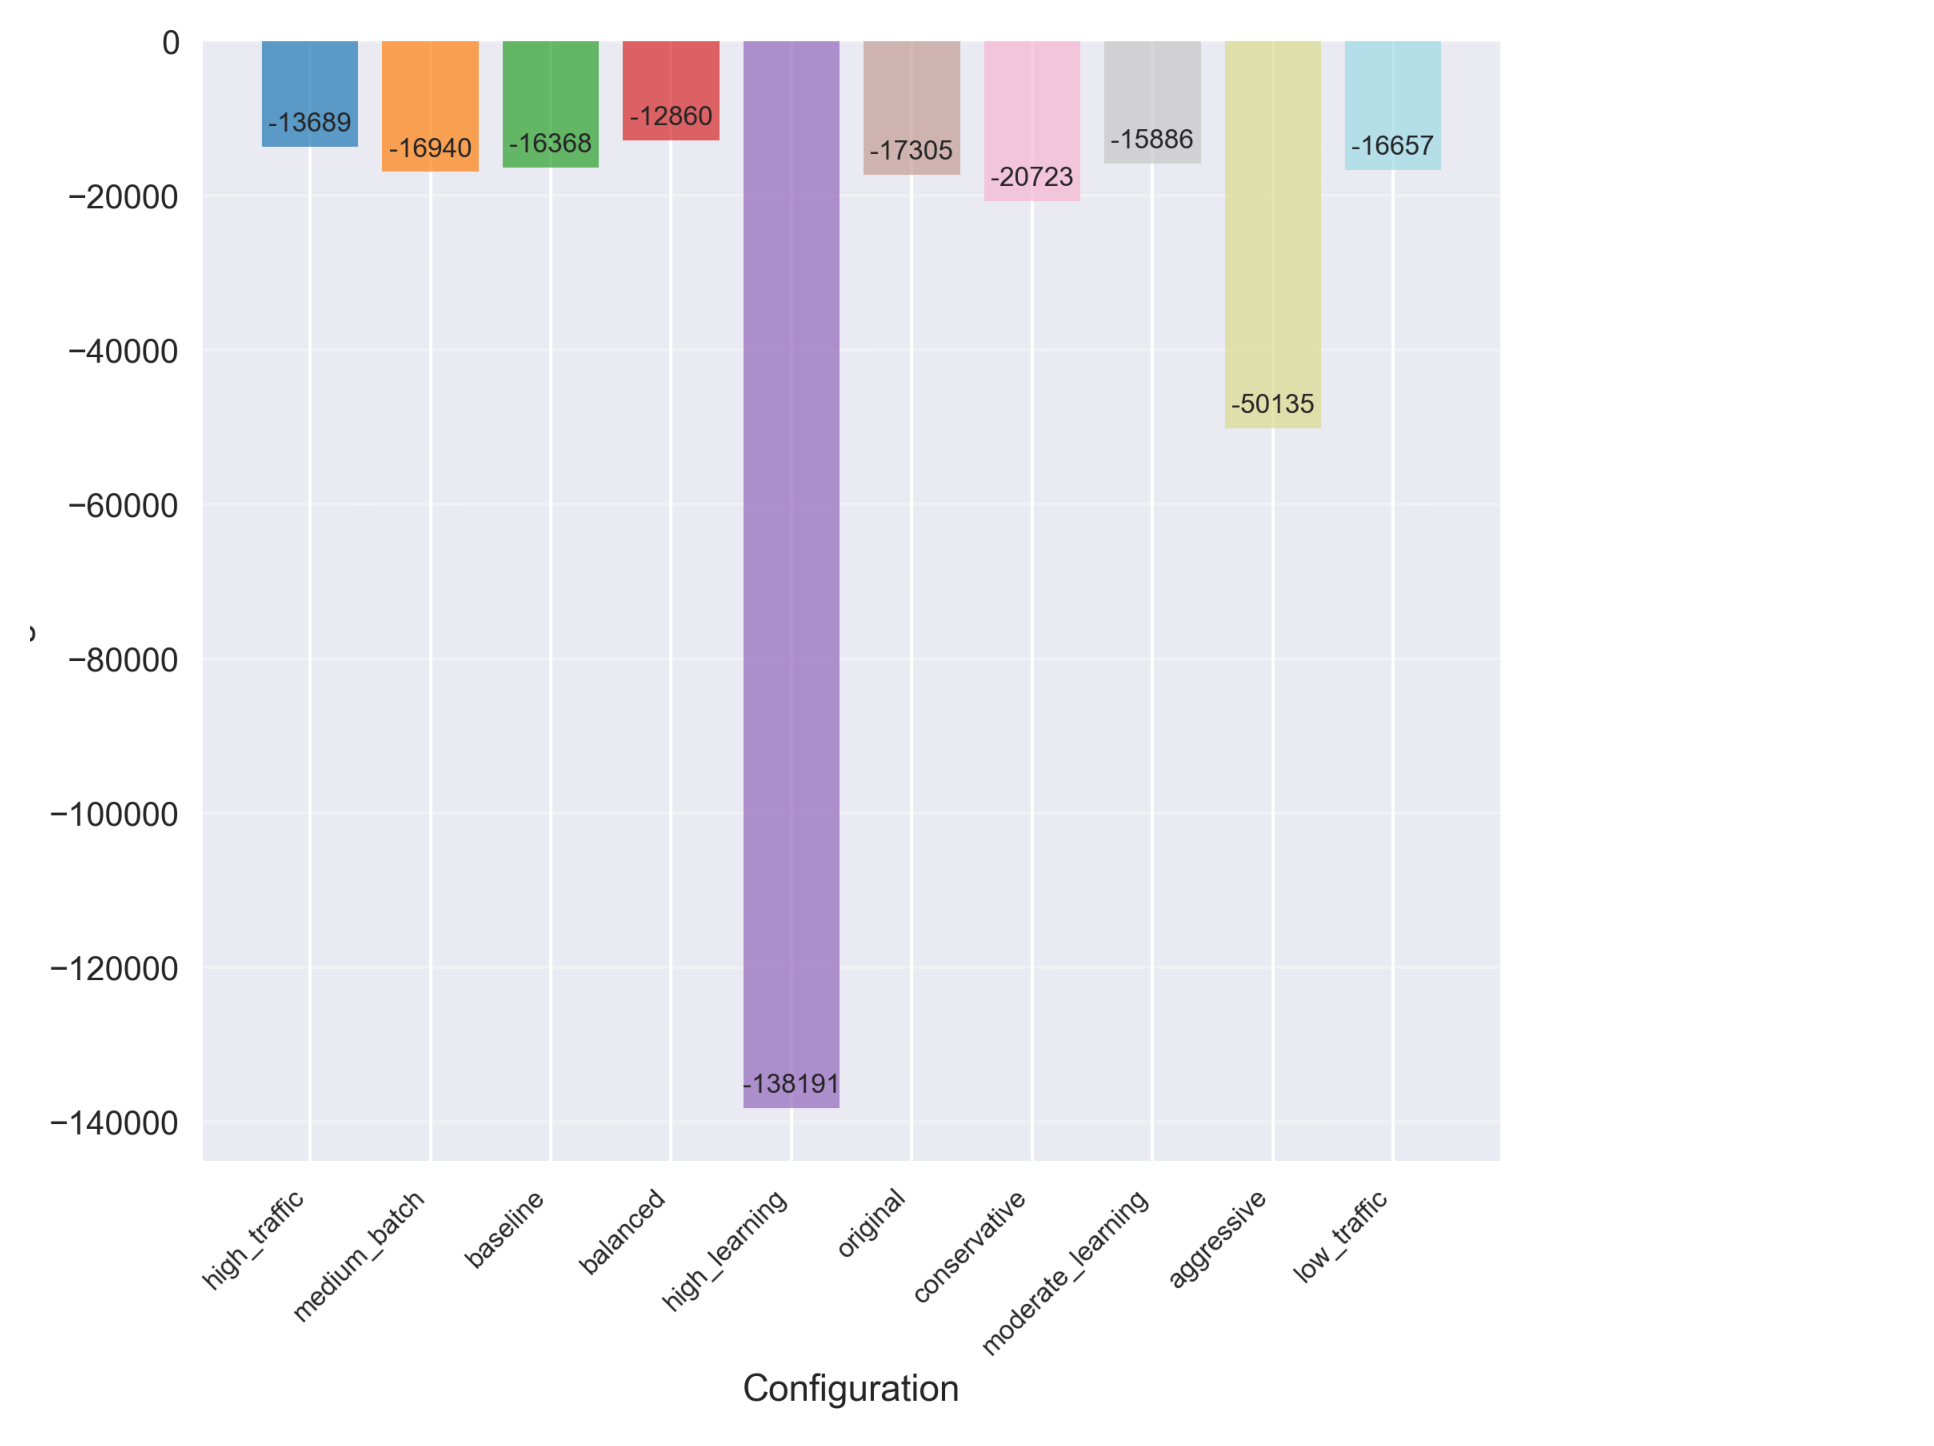
\includegraphics[width=\textwidth]{
        figures/individual_plots/intersection_full_performance_summary.png
    }
    \caption{Tổng hợp so sánh hiệu suất tất cả 10 mô hình intersection agent}
    \label{fig:intersection_full_performance_summary}
\end{figure}

Hình \ref{fig:intersection_full_performance_summary} tổng hợp đầy đủ kết quả của
tất cả 10 mô hình. Kết quả cho thấy rõ ràng sự thay đổi đáng kề khi lựa chọn
tham số không phù hợp: mô hình Aggressive đạt phần thưởng -50,135 (kém 290\% so với
Balanced), trong khi High Learning đạt -138,191 (kém 975\% so với Balanced).
Điều này nhấn mạnh tầm quan trọng của việc lựa chọn siêu tham số cẩn thận
trong Deep Reinforcement Learning.

\subsection{Hiệu suất của mô hình tối ưu}

Mô hình \textbf{Balanced} thể hiện hiệu suất vượt trội với các chỉ số sau:

\begin{align}
    \text{Phần thưởng trung bình}     & : -12,860.19             \\
    \text{Thời gian chờ trung bình}   & : 37,505.85 \text{ giây} \\
    \text{Độ dài hàng đợi trung bình} & : 6.95 \text{ xe}
\end{align}

Kết quả này cho thấy mô hình Balanced không chỉ đạt được hiệu suất cao mà còn duy
trì sự ổn định trong suốt quá trình hoạt động.

\subsection{So sánh tổng thể giao lộ đơn}

Bảng dưới đây tổng hợp kết quả so sánh hiệu suất của tất cả các mô hình, được sắp
xếp theo thứ tự từ tốt nhất đến kém nhất:

\begin{table}[!htp]
    \centering
    \caption{Kết quả so sánh hiệu suất các mô hình DQN}
    \label{tab:model_performance_comparison}
    \begin{tabular}{@{}lccc@{}}
        \toprule \textbf{Mô hình}  & \textbf{Phần thưởng TB} & \textbf{Thời gian chờ TB (s)} & \textbf{Độ dài hàng đợi TB} \\
        \midrule \textbf{Balanced} & \textbf{-12,860.19}     & \textbf{37,505.85}            & \textbf{6.95}               \\
        High Traffic               & -13,688.96              & 38,012.28                     & 7.04                        \\
        Moderate Learning          & -15,886.35              & 41,012.58                     & 7.59                        \\
        Baseline                   & -16,367.69              & 41,404.70                     & 7.67                        \\
        Low Traffic                & -16,656.51              & 43,583.13                     & 8.07                        \\
        Original                   & -17,304.83              & 44,697.74                     & 8.28                        \\
        Medium Batch               & -16,940.37              & 43,315.68                     & 8.02                        \\
        Conservative               & -20,723.03              & 46,952.09                     & 8.69                        \\
        Aggressive                 & -50,134.78              & 172,687.93                    & 31.98                       \\
        High Learning              & -138,190.51             & 61,483.15                     & 11.39                       \\
        \bottomrule
    \end{tabular}
\end{table}

\section{Phát triển và thực nghiệm Sync Agent}

\subsection{Thách thức trong phát triển Sync Agent}

Sync Agent là một thành phần hoàn toàn mới được thiết kế từ đầu để giải quyết
bài toán đồng bộ hóa tín hiệu giao thông đa giao lộ. Quá trình phát triển đã gặp
phải các thách thức kỹ thuật quan trọng:

\subsubsection{Vấn đề huấn luyện không ổn định ban đầu}

Quá trình huấn luyện ban đầu đã thể hiện sự không ổn định đáng kể, đặc trưng bởi các vấn đề sau:

\begin{itemize}
    \item \textbf{Biến động phần thưởng cực đoan:} Hệ số biến thiên của phần thưởng vượt quá $2.10$, cho thấy một quá trình huấn luyện kém ổn định.
    \item \textbf{Phạm vi phần thưởng rộng:} Phần thưởng dao động dữ dội, từ $-3,200$ đến $+2,667$, tổng phạm vi xấp xỉ $6,000$ đơn vị.
    \item \textbf{Tỷ lệ cao các biến động lớn:} Khoảng $27.3\%$ số tập huấn luyện đã trải qua các biến động lớn, không mong muốn về phần thưởng.
    \item \textbf{Điểm chất lượng huấn luyện thấp:} Chất lượng huấn luyện tổng thể kém, chỉ đạt $25/100$ điểm.
\end{itemize}

\begin{algorithm}[!htp]
    \caption{Phân tích và cải thiện độ ổn định huấn luyện}
    \begin{algorithmic}[1]
        \State \textbf{Pha 1: Chẩn đoán}
        \State coefficient\_variation = $\frac{\text{std}(\text{rewards})}{|\text{mean}(\text{rewards})|}$
        \State large\_swings\_percentage = $\frac{\text{count}(|\text{reward\_changes}| > \text{threshold})}{\text{total\_episodes}}$
        \State trend\_analysis = linear\_regression(rewards, episodes)
        \State quality\_score = compute\_overall\_quality(stability\_metrics)
        
        \State \textbf{Pha 2: Kỹ thuật phần thưởng cực kỳ ổn định}
        \If{quality\_score $<$ 50}
            \State implement\_long\_term\_comparison()
            \State apply\_non\_overlapping\_windows()
            \State use\_percentage\_based\_improvements()
            \State apply\_sigmoid\_transformation()
        \EndIf
        
        \State \textbf{Pha 3: Điều chỉnh siêu tham số thận trọng}
        \State learning\_rate = reduce\_by\_factor(current\_lr, 0.3)
        \State discount\_factor = reduce\_to\_conservative(0.95)
        \State network\_size = reduce\_complexity(128, 128)
        \State target\_update\_tau = slow\_down\_to(0.001)
    \end{algorithmic}
\end{algorithm}

\subsection{Cấu hình reward structures cho Sync Agent}

Một trong những đóng góp quan trọng của nghiên cứu là việc phát triển và so sánh
hai cấu trúc phần thưởng khác nhau:

\subsubsection{Positive Reward Model (Sync Coordination Approach)}
\begin{itemize}
    \item \textbf{Công thức tính phần thưởng:} \texttt{reward = old\_waiting\_time -         current\_waiting\_time}

    \item \textbf{Phương pháp đo lường:} So sánh thời gian chờ đợi dựa trên snapshot

    \item \textbf{Phạm vi giá trị:}  Có thể đạt cả giá trị dương và âm

    \item \textbf{Diễn giải:} Phần thưởng dương = đồng bộ thành công
\end{itemize}

\subsubsection{Negative Reward Model (Intersection Agent Style)}
\begin{itemize}
    \item \textbf{Công thức tính phần thưởng:} \texttt{reward = old\_cumulative\_wait -
        new\_cumulative\_wait}

    \item \textbf{Phương pháp đo lường:} Thời gian chờ tích lũy (luôn tăng)

    \item \textbf{Phạm vi giá trị:} Luôn âm (ít âm hơn = hiệu suất tốt hơn)

    \item \textbf{Diễn giải:}  Theo phương pháp intersection agent đã được
        thiết lập
\end{itemize}

\section{Kết quả thực nghiệm Sync Agent}

\subsection{So sánh hai cấu trúc phần thưởng}

Nghiên cứu đã tiến hành huấn luyện 150 tập huấn luyện cho mỗi cấu trúc phần thưởng và thu được
kết quả đáng kể:

\subsection{So sánh chi tiết hiệu suất hai mô hình}

\subsubsection{Tiến trình phần thưởng}

\begin{figure}[!htp]
    \centering
    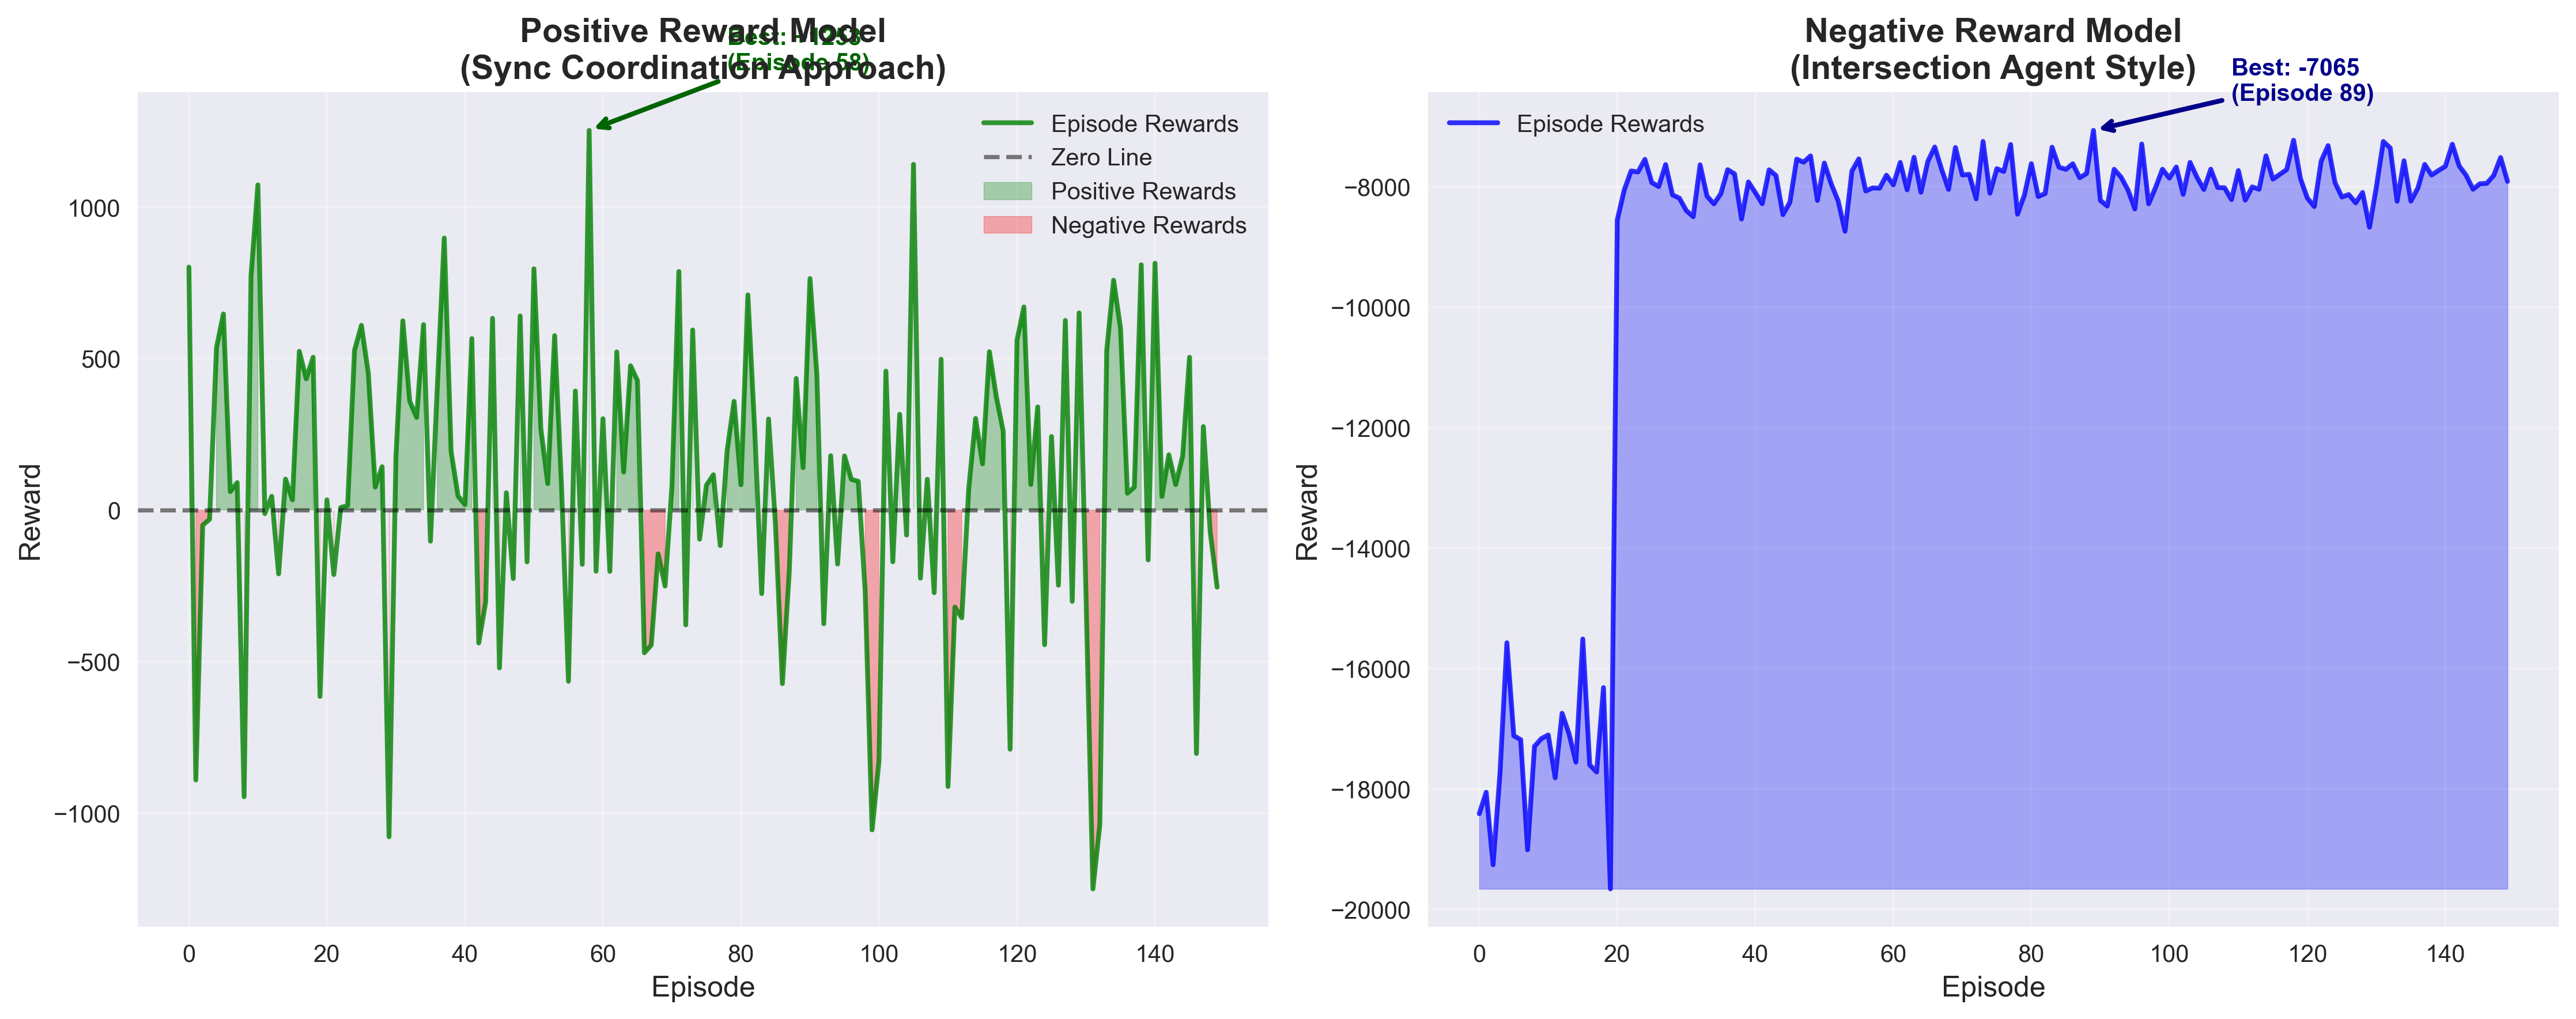
\includegraphics[width=\textwidth]{figures/sync_reward_comparison.png}
    \caption{So sánh tiến trình phần thưởng giữa hai mô hình Sync Agent}
    \label{fig:sync_reward_comparison}
\end{figure}

Hình \ref{fig:sync_reward_comparison} thể hiện sự khác biệt rõ rệt trong tiến
trình học của hai mô hình. Positive Reward Model cho thấy khả năng đạt được phần thưởng
dương, với hiệu năng cao nhất tại tập huấn luyện 58 (+1,253.11), trong khi Negative
Reward Model duy trì xu hướng cải thiện ổn định.

\subsubsection{Thời gian chờ đợi}

\begin{figure}[!htp]
    \centering
    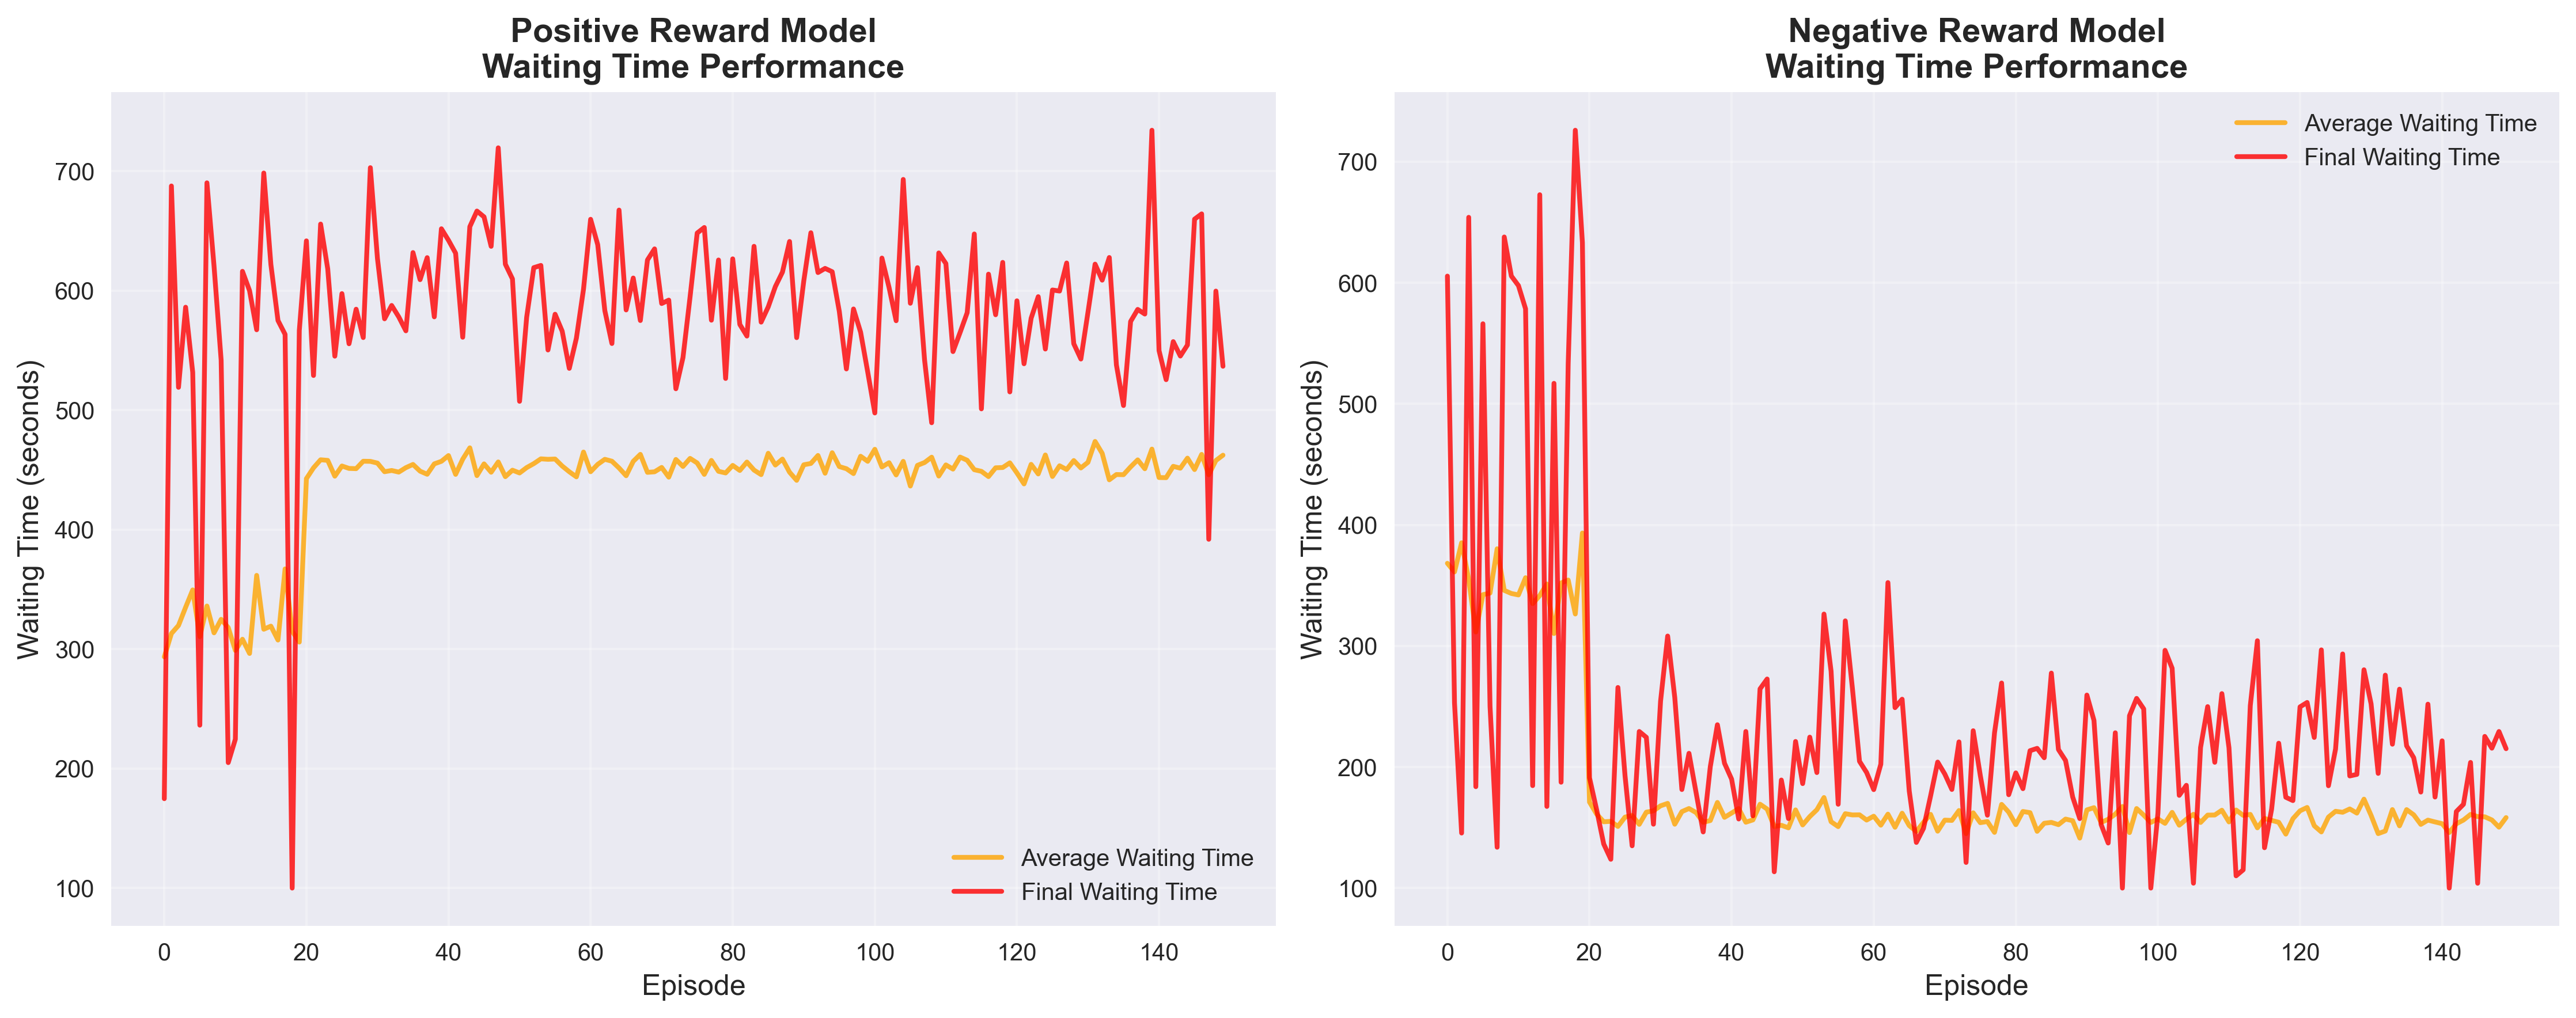
\includegraphics[width=\textwidth]{figures/sync_waiting_time_comparison.png}
    \caption{So sánh thời gian chờ đợi giữa hai mô hình Sync Agent}
    \label{fig:sync_waiting_time_comparison}
\end{figure}

Hình \ref{fig:sync_waiting_time_comparison} cho thấy Negative Reward Model đạt
hiệu suất vượt trội về thời gian chờ đợi, với giá trị tốt nhất 141.30s so với
293.46s của Positive Reward Model.

\subsubsection{Đường cong học tập}

\begin{figure}[!htp]
    \centering
    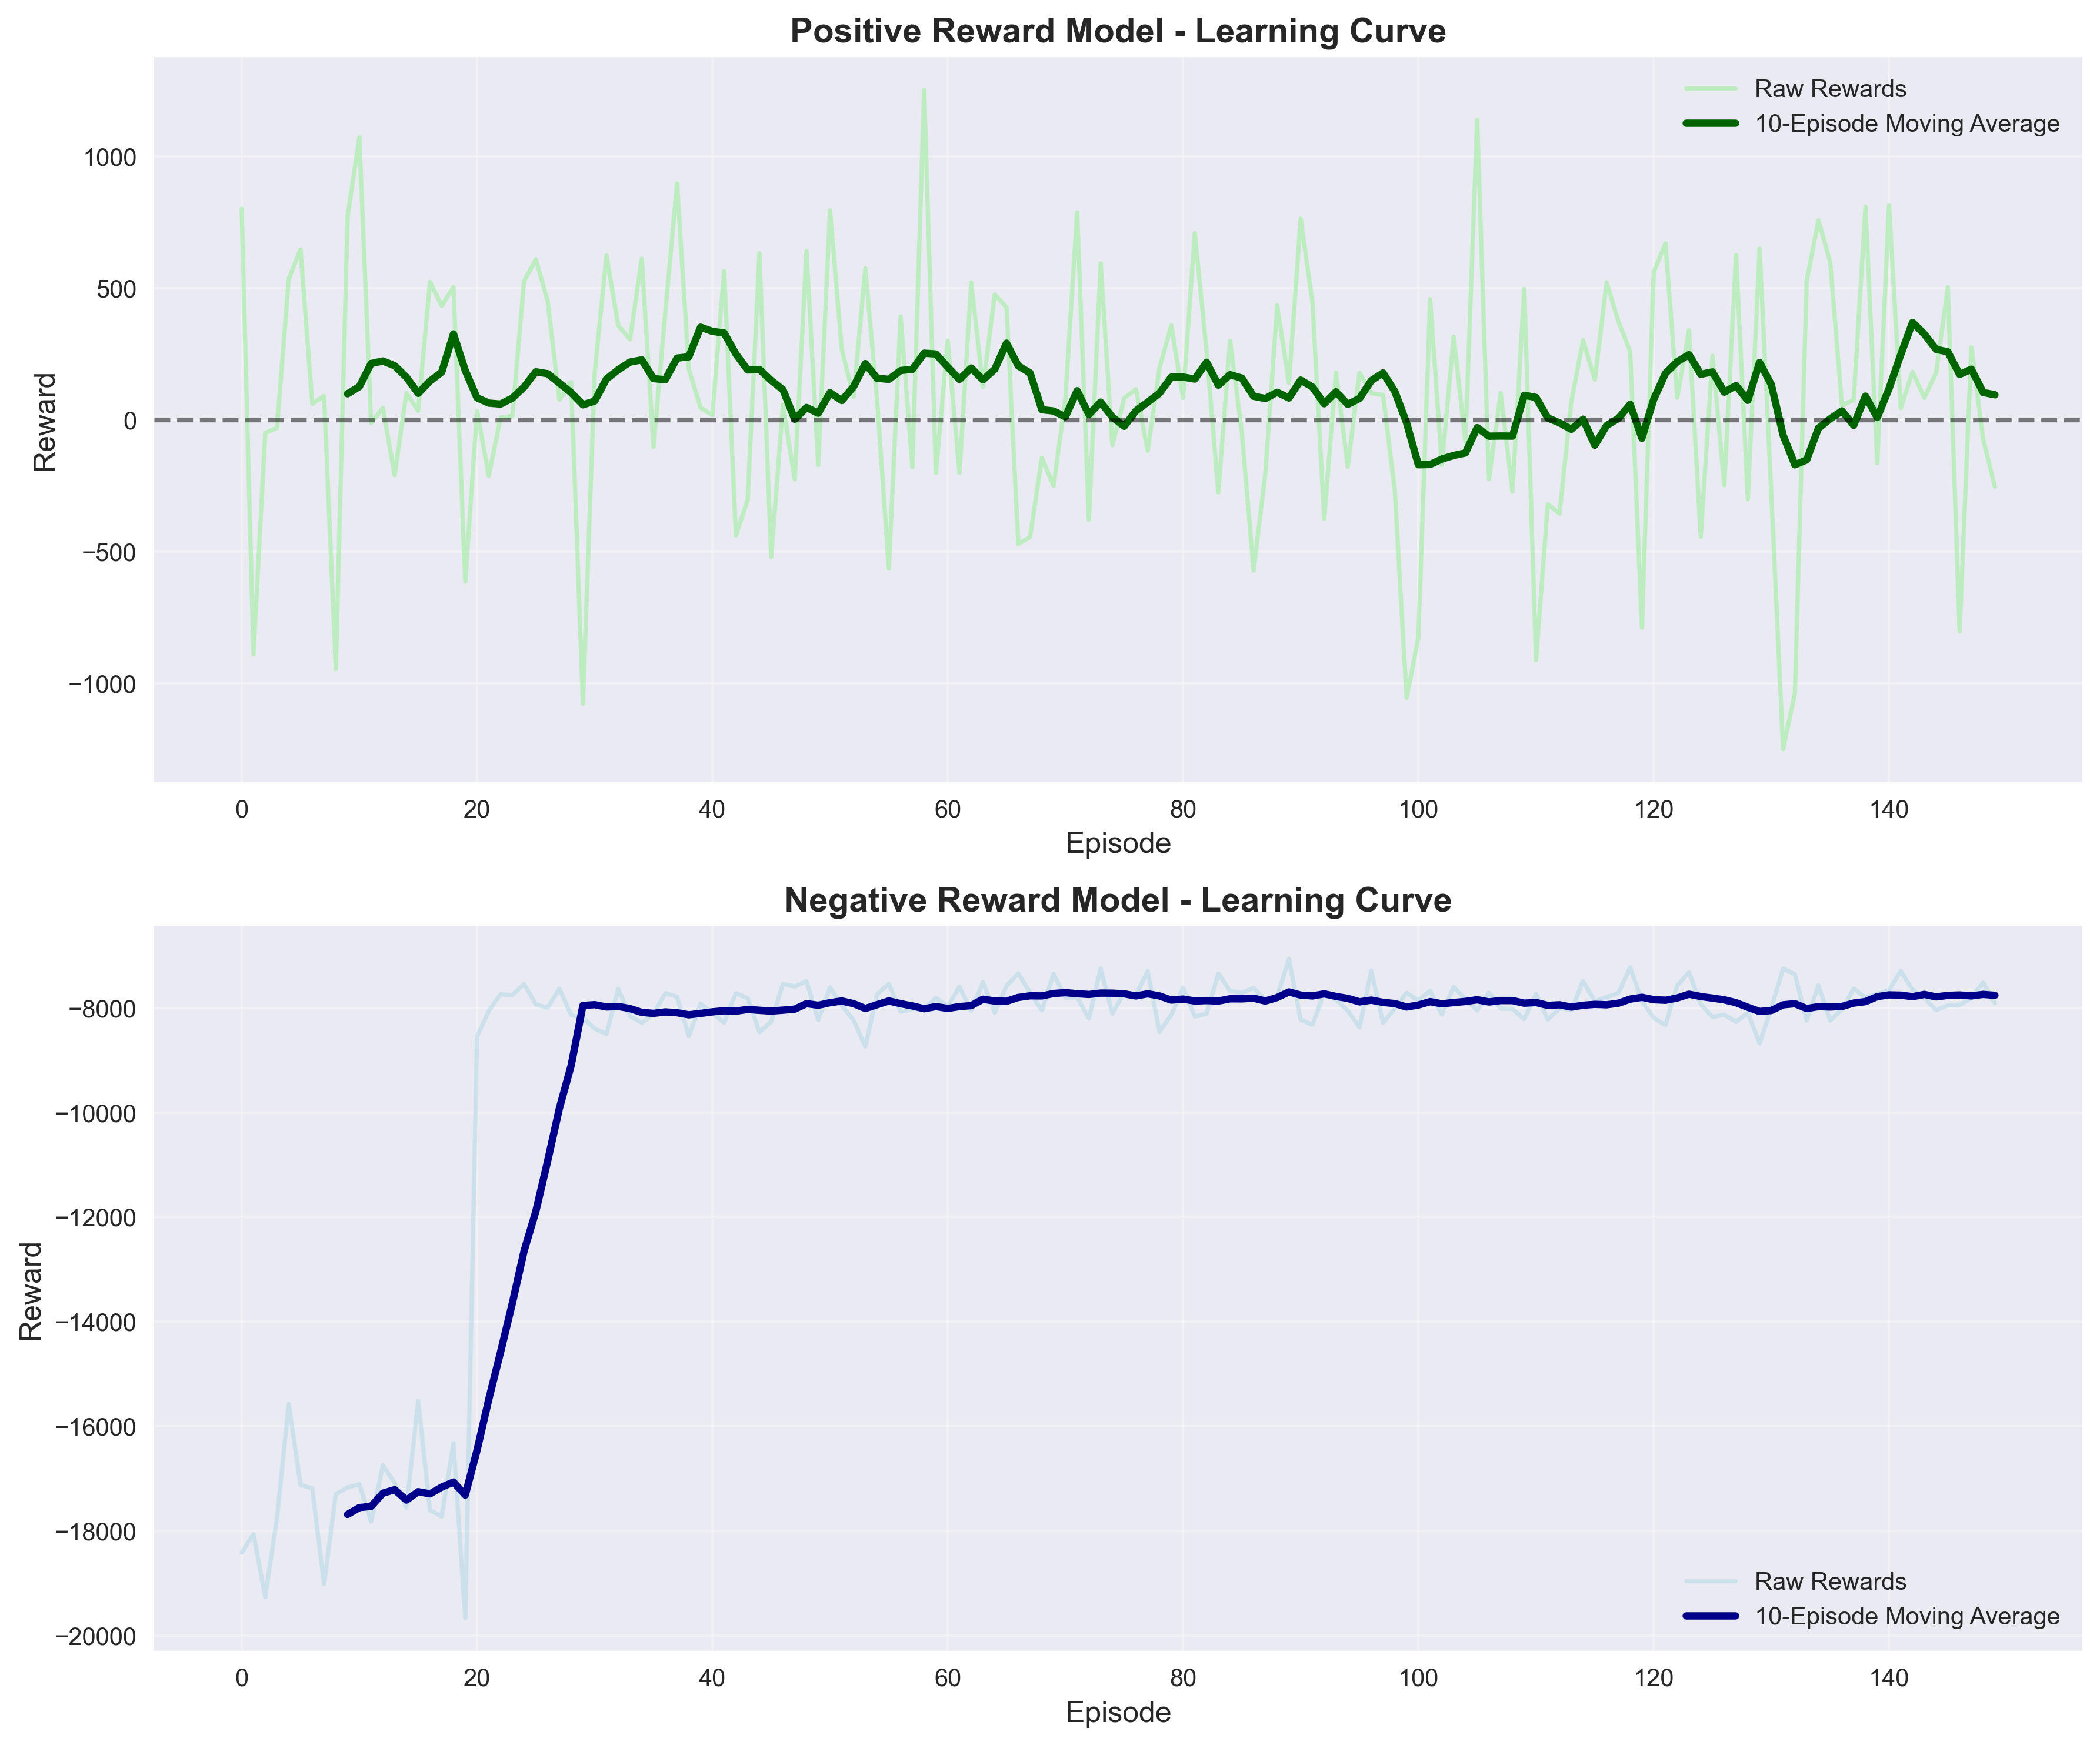
\includegraphics[width=\textwidth]{figures/sync_learning_curves.png}
    \caption{Đường cong học tập của hai mô hình Sync Agent}
    \label{fig:sync_learning_curves}
\end{figure}
Hình \ref{fig:sync_learning_curves} minh họa các khuôn mẫu học tập khác biệt
giữa hai mô hình: Mô hình Positive Reward cho thấy các
chu kỳ rõ ràng giữa phản hồi tích cực và tiêu cực, trong khi mô hình Negative Reward Model thể hiện một đường cong học tập ổn định hơn.
\subsection{Phân tích kết quả hiệu suất}

\begin{table}[!htp]
    \centering
    \caption{So sánh hiệu suất của hai cấu trúc phần thưởng trong mô hình Sync Agent}
    \label{tab:sync_performance_comparison}
    \begin{tabular}{@{}lcc@{}}
        \toprule
        \textbf{Chỉ số} & \textbf{Mô hình Phần thưởng Dương} & \textbf{Mô hình Phần thưởng Âm} \\
        \midrule
        Phần thưởng tốt nhất      & $+1,253.11$                      & $-7,064.85$                      \\
        Phần thưởng cuối cùng     & $-254.30$                        & $-7,911.73$                      \\
        Phần thưởng trung bình    & $+106.35$                        & $-8,169.63$                      \\
        Độ lệch chuẩn phần thưởng & $471.23$                         & $3,314.12$                       \\
        Thời gian chờ TB tốt nhất & $293.46$s                        & $141.30$s                        \\
        Thời gian chờ TB cuối cùng & $462.23$s                        & $158.23$s                        \\
        Số tập có cải thiện       & $97$ tập                         & Giảm thiểu nhất quán            \\
        Tập đạt hiệu suất cao nhất & Tập $58$                         & Tập $89$                         \\
        \bottomrule
    \end{tabular}
\end{table}

\subsection{Kết quả chi tiết từng mô hình}

\subsubsection{Hiệu suất mô hình Positive Reward}

\begin{figure}[!htp]
    \centering
    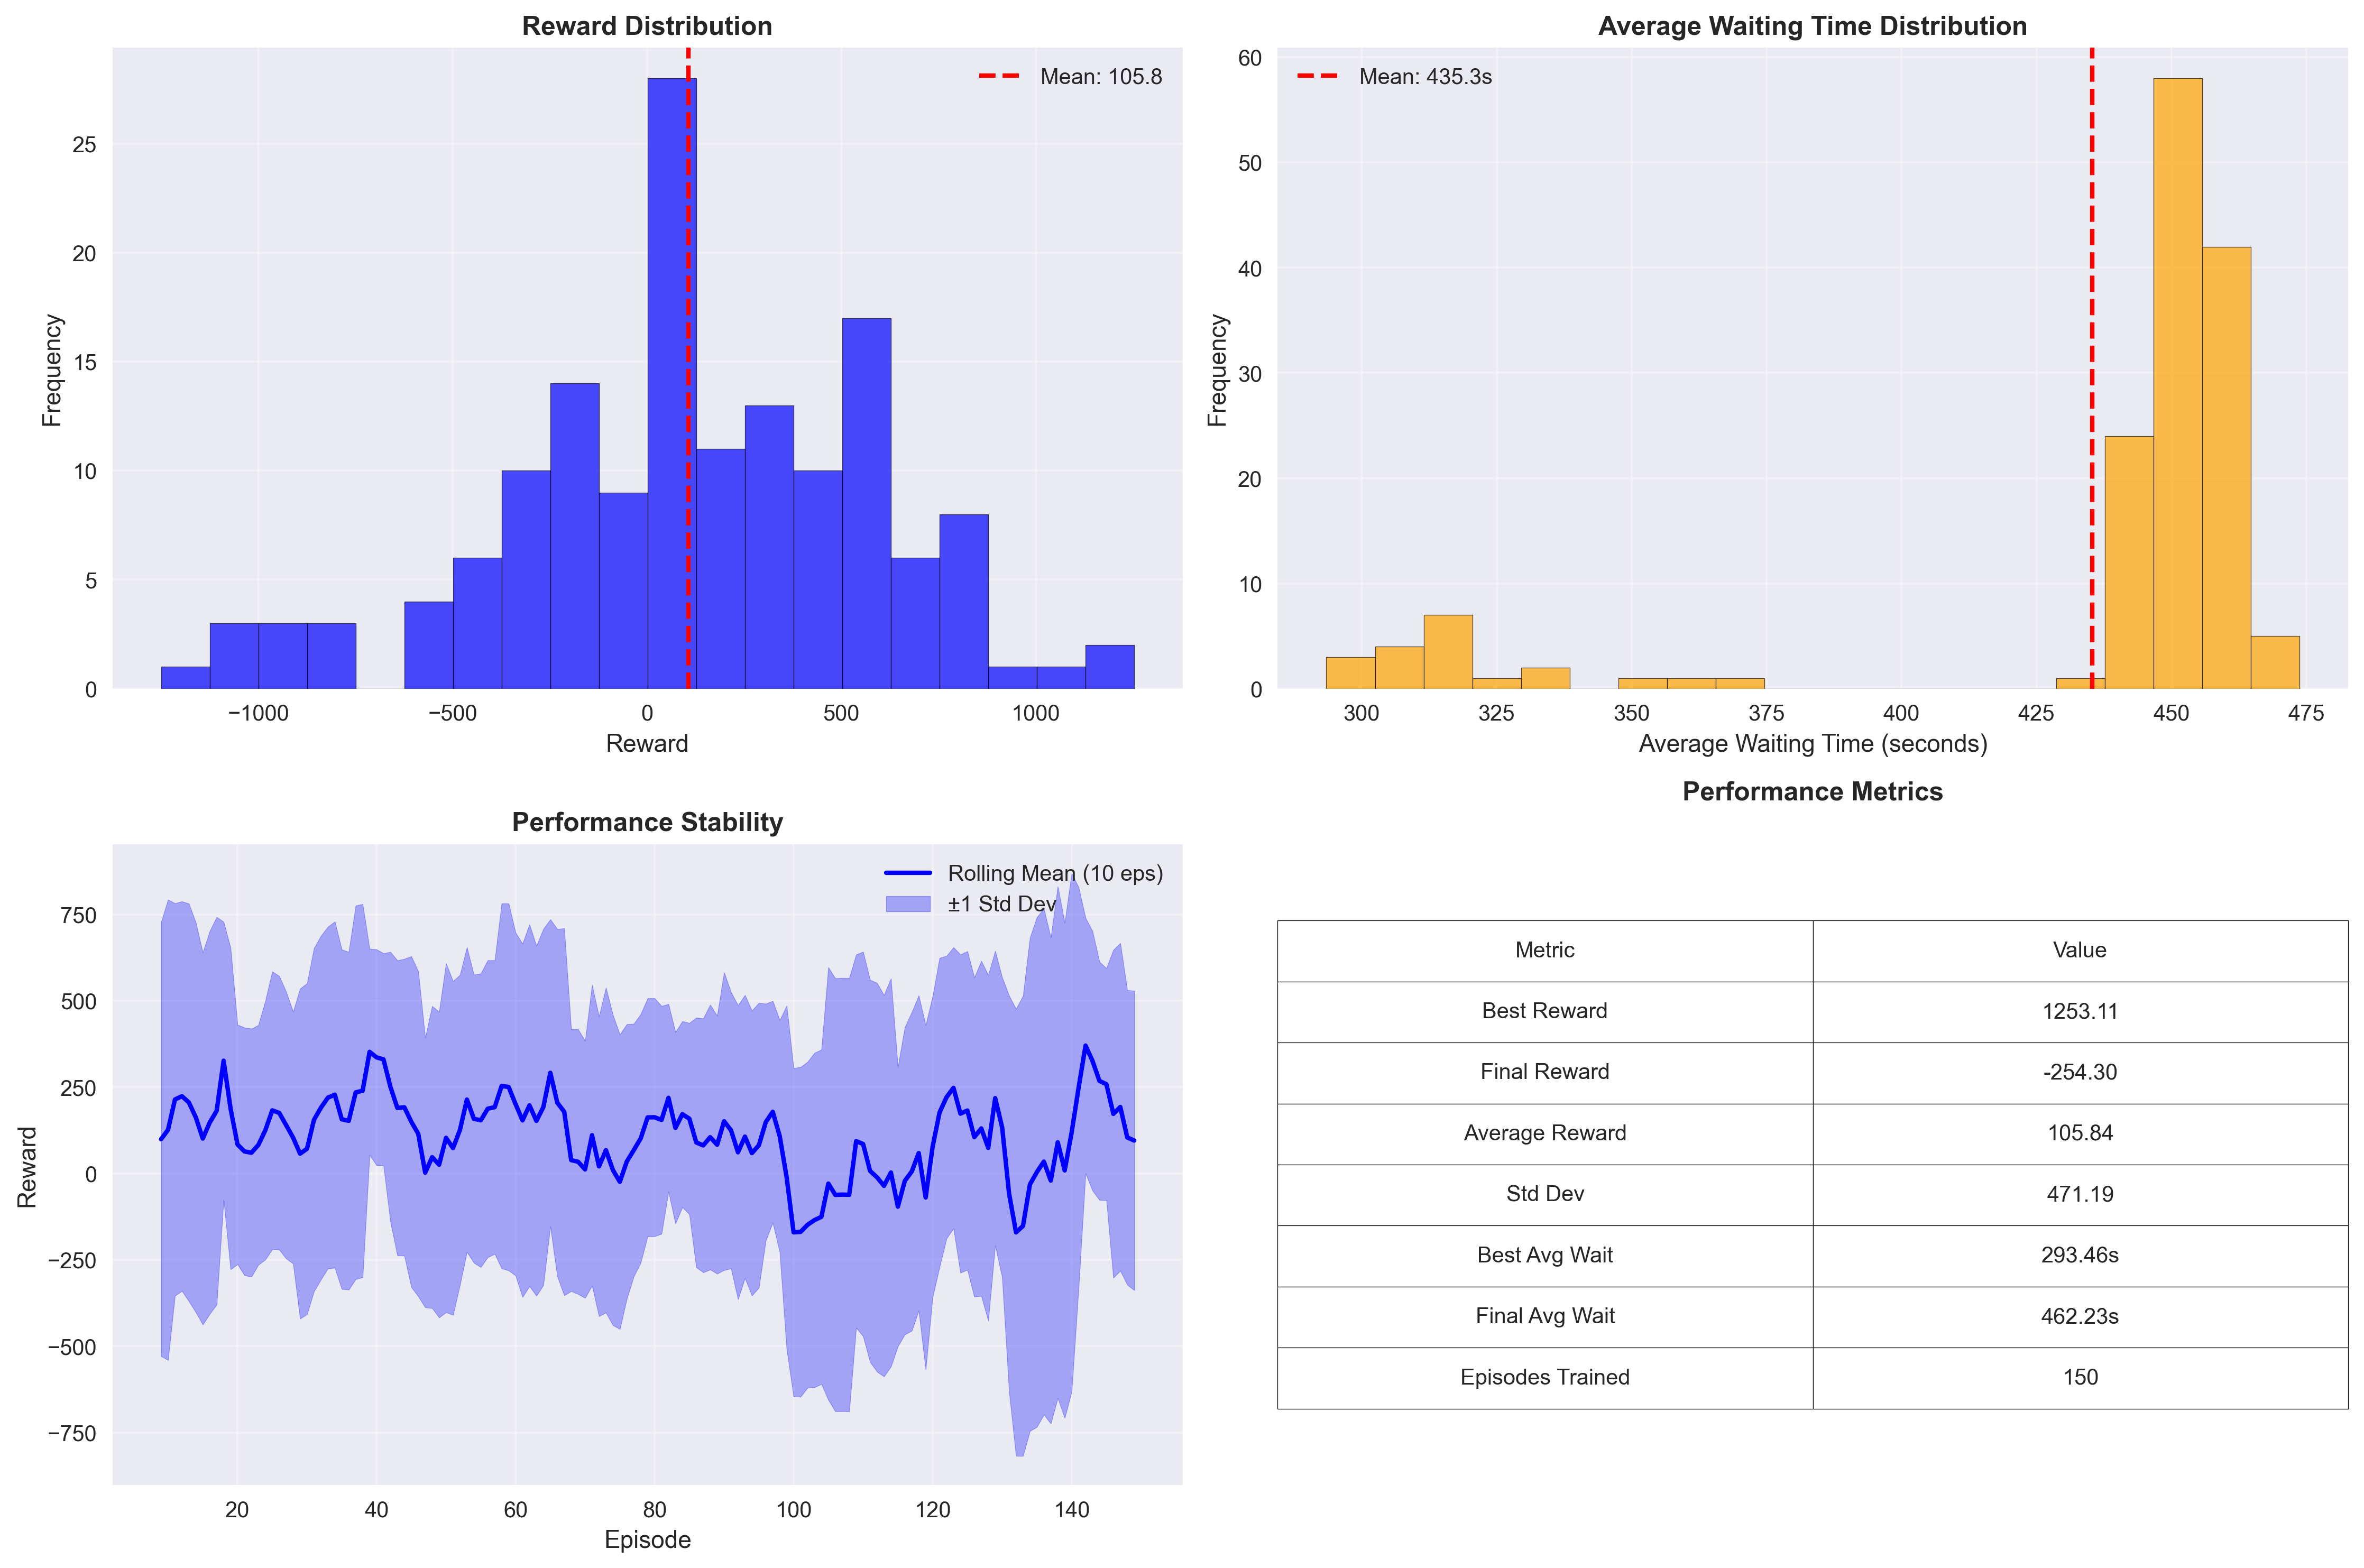
\includegraphics[width=\textwidth]{figures/sync_positive_model_summary.png}
    \caption{Phân tích chi tiết hiệu suất Positive Reward Model}
    \label{fig:sync_positive_model_summary}
\end{figure}

Mô hình Positive Reward đạt được:
\begin{itemize}
    \item \textbf{Hiệu suất cao nhất:} Episode 58 với phần thưởng +1,253.11

    \item \textbf{Hành vi học:} Các chu kỳ rõ ràng giữa phản hồi dương/âm

    \item \textbf{Hội tụ:} Cải thiện theo từng tập huấn luyện với các lần lỗi

    \item \textbf{Thời gian chờ đợi:} 293s - 474s

    \item \textbf{Chứng minh đồng bộ hóa:} Phần thưởng dương chỉ ra sự thành công
        của đồng bộ hóa
\end{itemize}

\subsubsection{Hiệu suất mô hình Negative Reward}

\begin{figure}[!htp]
    \centering
    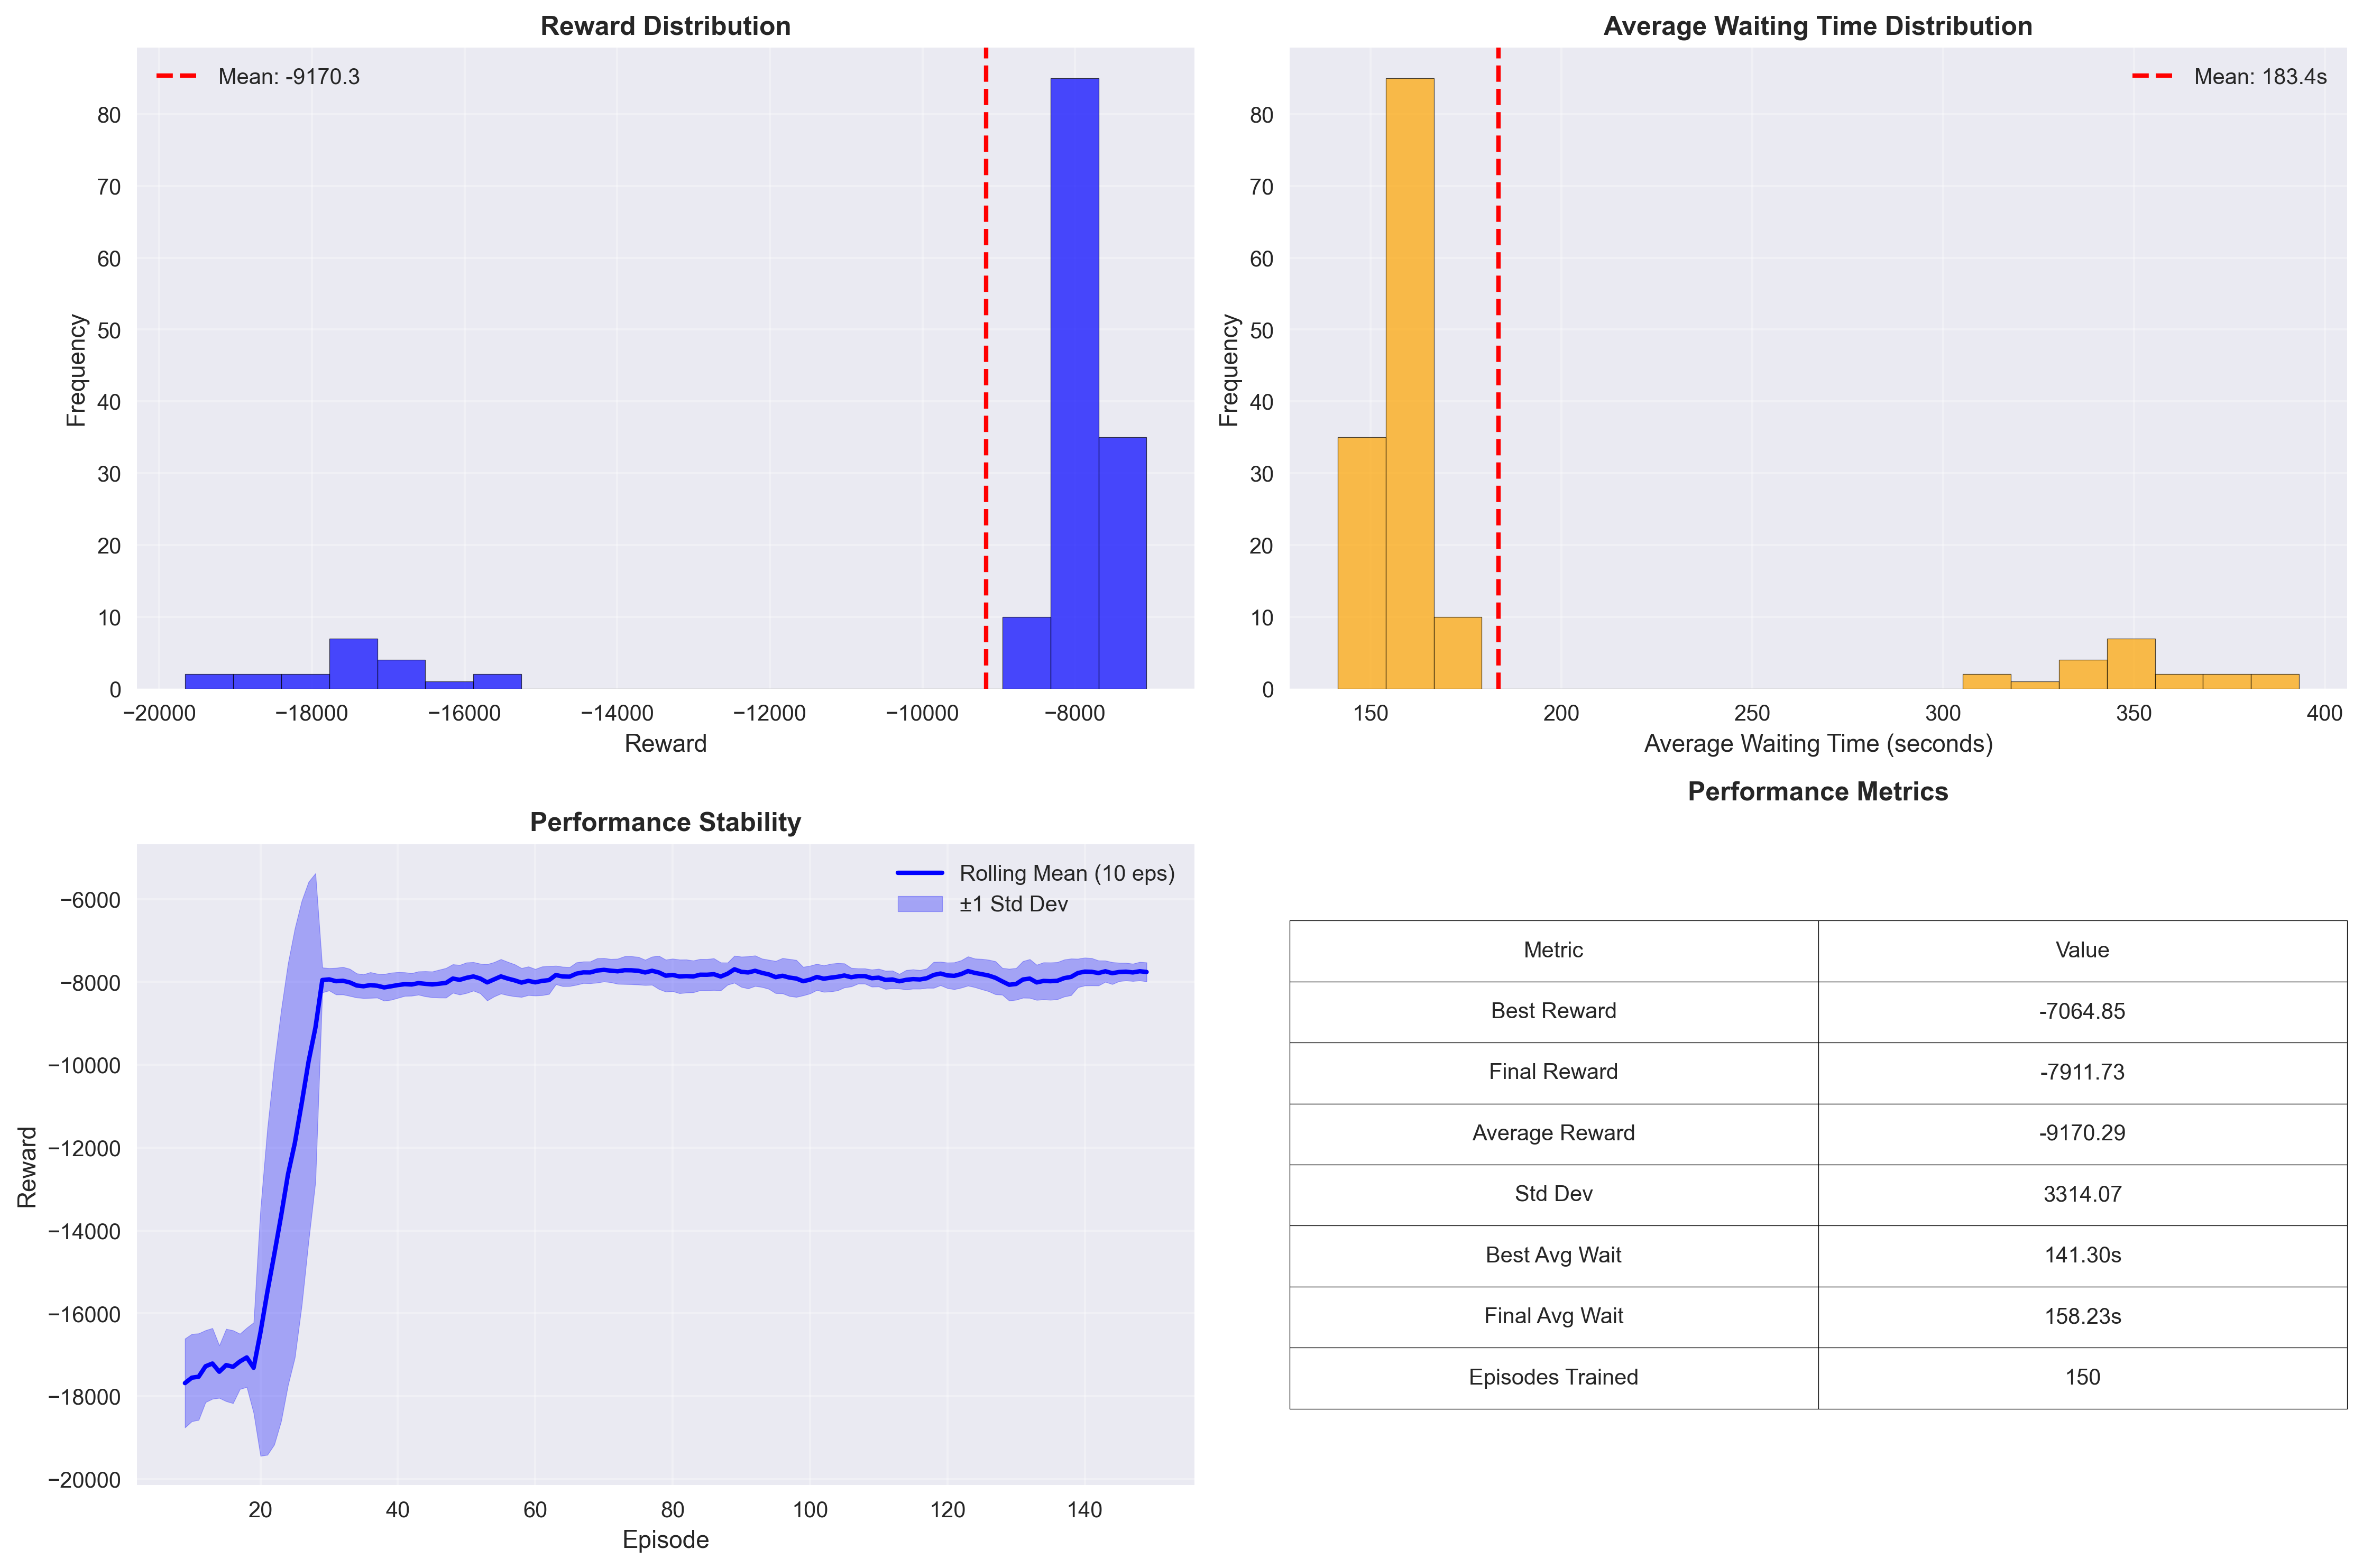
\includegraphics[width=\textwidth]{figures/sync_negative_model_summary.png}
    \caption{Phân tích chi tiết hiệu suất Negative Reward Model}
    \label{fig:sync_negative_model_summary}
\end{figure}

Mô hình Negative Reward đạt được:
\begin{itemize}
    \item \textbf{Hiệu suất cao nhất:} Episode 89 với phần thưởng -7,064.85

    \item \textbf{Hành vi học:} Phần thưởng âm với cải thiện từ từ
        improvement

    \item \textbf{Hội tụ:} Đường cong học tập ổn định, tương tự intersection agents

    \item \textbf{Thời gian chờ đợi:} 141s - 393s

    \item \textbf{Quản lý giao thông:} Hiệu suất thời gian chờ đợi tốt hơn
\end{itemize}

\subsection{Comprehensive Performance Metrics}

\begin{figure}[!htp]
    \centering
    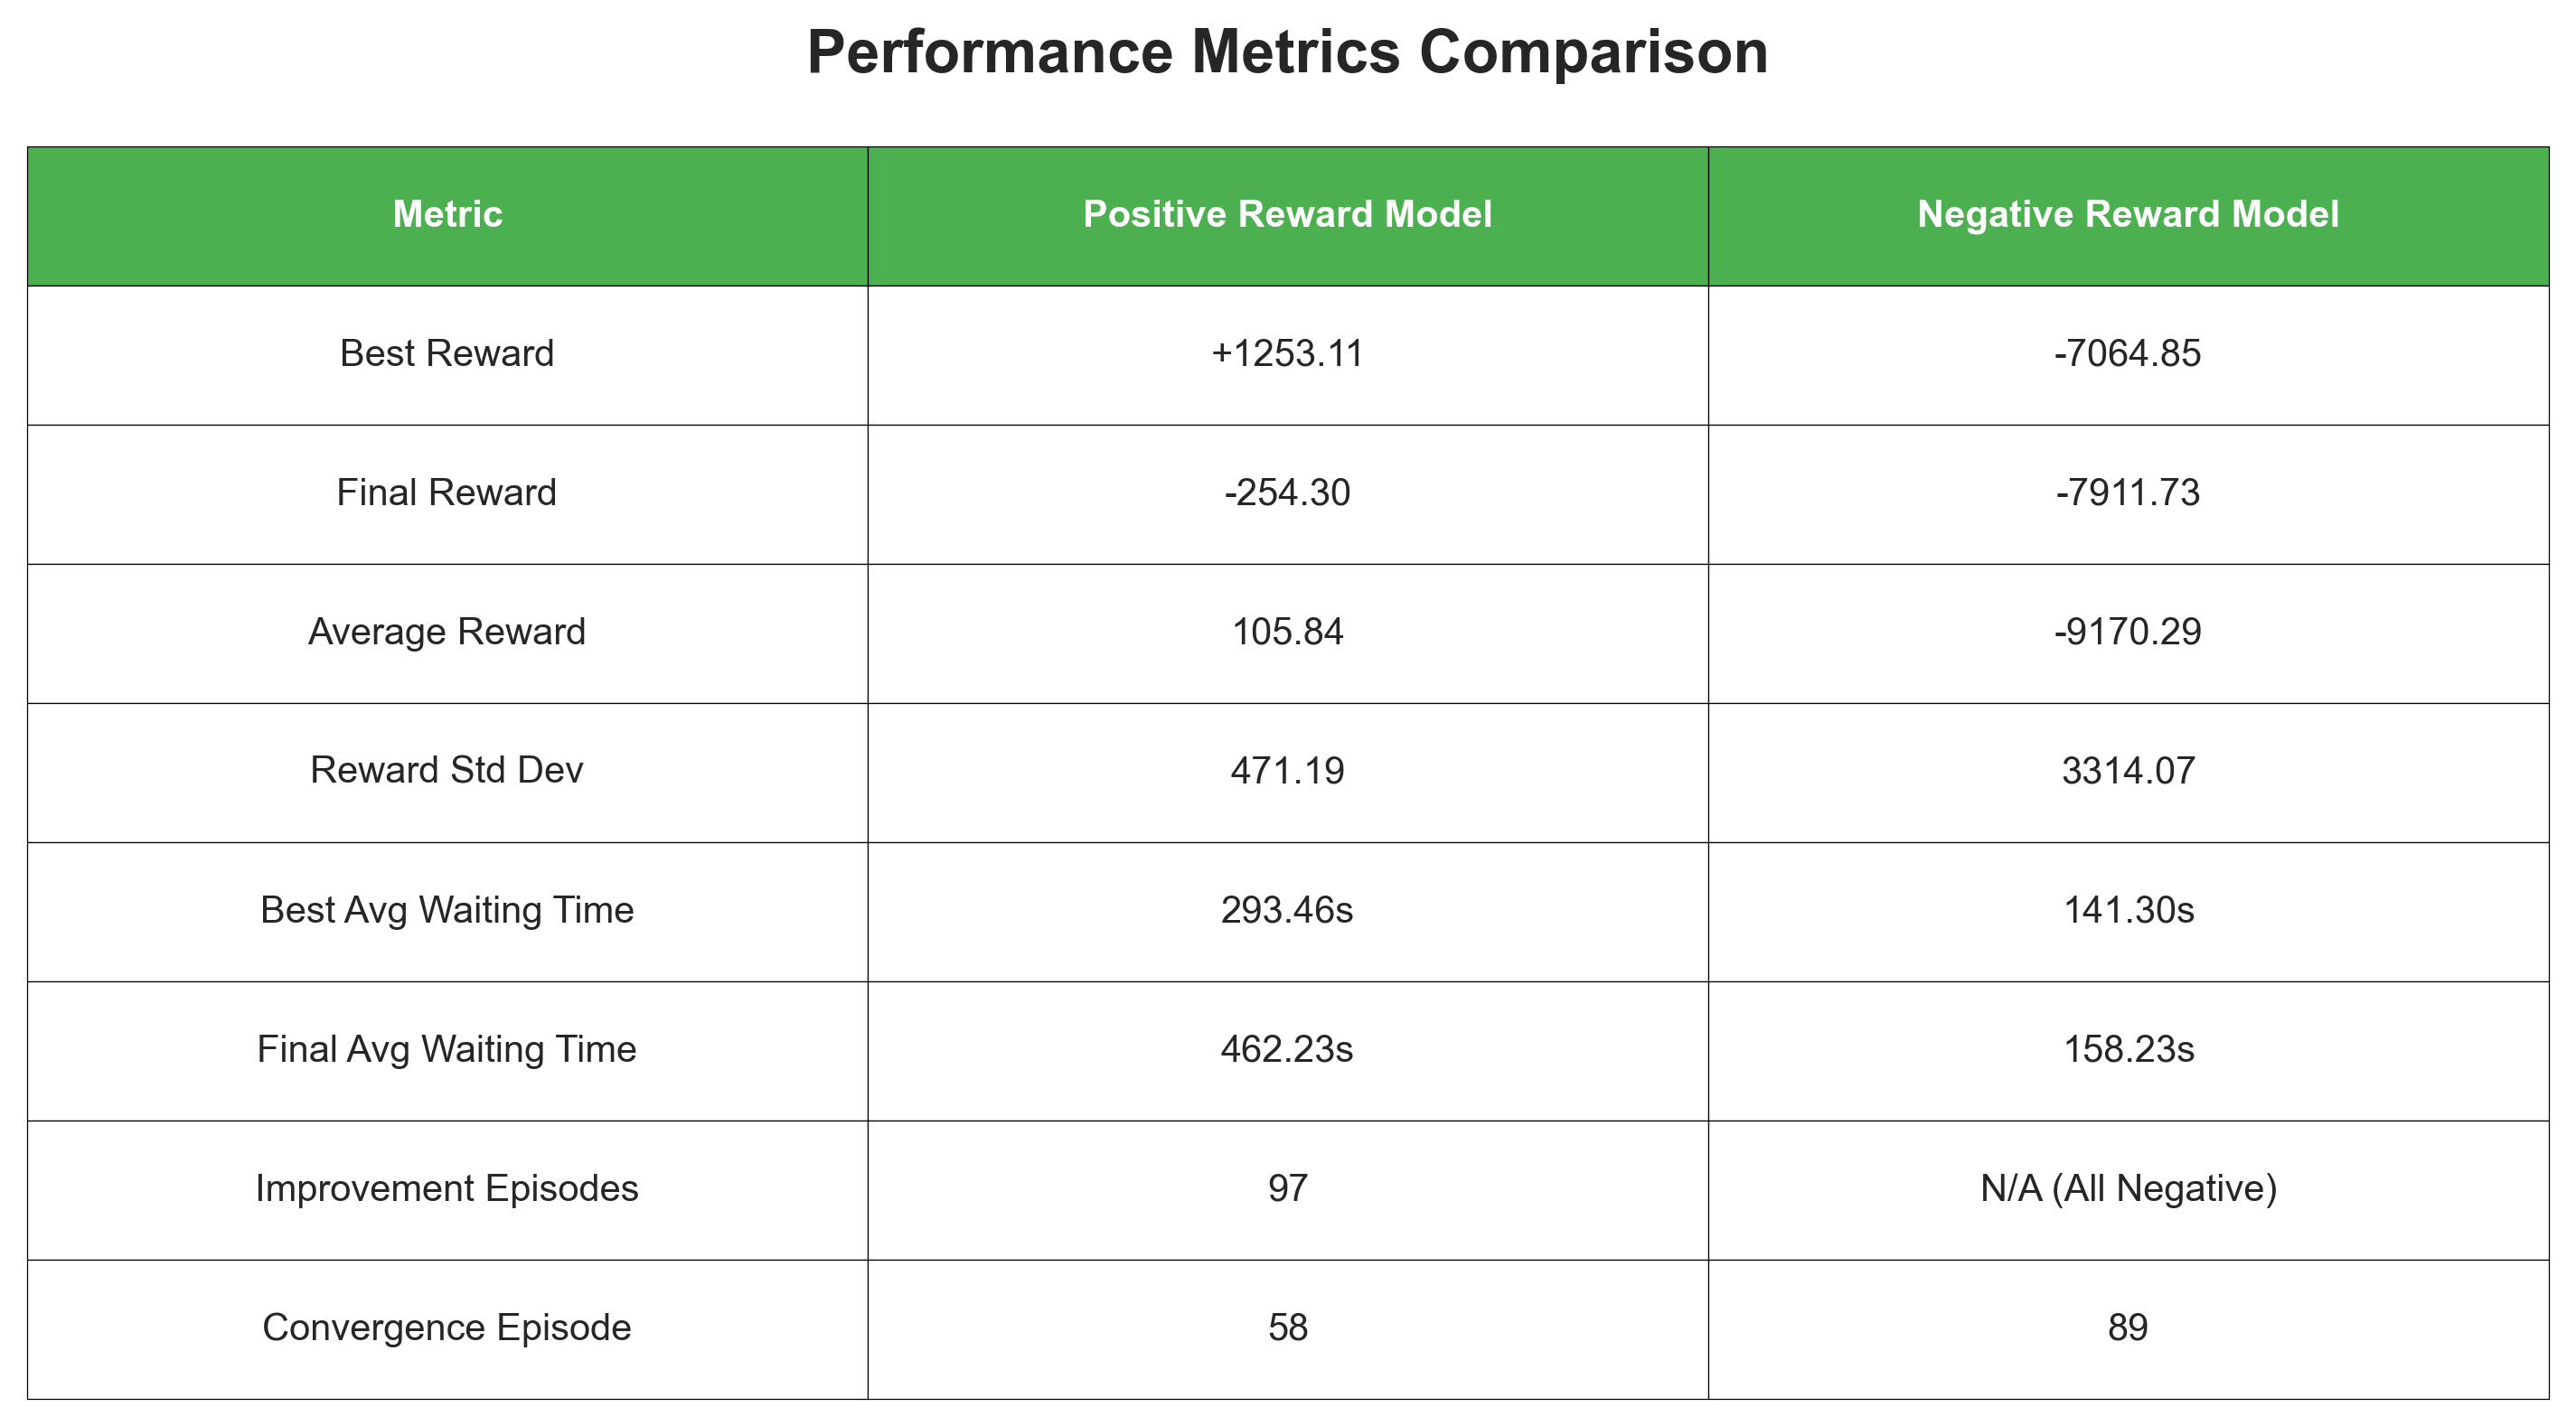
\includegraphics[width=\textwidth]{figures/sync_performance_metrics.png}
    \caption{Bảng tổng hợp các chỉ số hiệu suất chi tiết của hai mô hình Sync Agent}
    \label{fig:sync_performance_metrics}
\end{figure}

\section{Phân tích kỹ thuật và insight}

\subsection{Phân tích và lựa chọn cấu trúc reward function}

Nghiên cứu đã thực hiện so sánh chi tiết hai cấu trúc phần thưởng khác nhau
để xác định phương pháp tối ưu cho Sync Agent. Việc lựa chọn cấu trúc phần thưởng có
tác động trực tiếp đến hiệu suất học và khả năng hội tụ của mô hình.

\subsubsection{Positive Reward Structure (Sync Coordination)}

\textbf{Nguyên lý hoạt động:} Positive reward structure được thiết kế để khuyến khích
các hành động đồng bộ hóa thành công:

\begin{align}
    R_{positive}= \begin{cases}+2.0&\text{nếu sync action thành công}\\ +1.0&\text{nếu coordination cải thiện traffic flow}\\ 0.0&\text{nếu không có thay đổi đáng kể}\\ -1.0&\text{nếu sync action gây tắc nghẽn}\\ -3.0&\text{nếu coordination hoàn toàn thất bại}\end{cases}
\end{align}

\textbf{Ưu điểm:}
\begin{itemize}
    \item \textbf{Phản hồi trực quan:} Agent dễ dàng hiểu positive = good, negative
        = bad

    \item \textbf{Khuyến khích khám phá:} Phần thưởng dương thúc đẩy agent thử
        nghiệm các chiến lược đồng bộ hóa

    \item \textbf{Phù hợp multi-agent:} Tối ưu cho các tình huống đồng bộ đa giao lộ

    \item \textbf{Hội tụ nhanh:} Agent học được các mẫu thành công một
        cách nhanh chóng
\end{itemize}

\textbf{Nhược điểm:}
\begin{itemize}
    \item \textbf{Phần thưởng thưa:} Không phải lúc nào cũng có đồng bộ hóa thành công để phần thưởng

    \item \textbf{Cực tiểu cục bộ:} Có thể bị kẹt ở các giải pháp cục bộ

    \item \textbf{Khó so sánh:} Không dễ dàng so sánh với các phương pháp đơn giao lộ
\end{itemize}

\subsubsection{Negative Reward Structure (Intersection Style)}

\textbf{Nguyên lý hoạt động:} Negative reward structure tập trung vào việc giảm
thiểu tổng thời gian chờ đợi của hệ thống:

\begin{align}
    R_{negative}= -\frac{\text{total\_waiting\_time}}{normalization\_factor}
\end{align}

Trong đó normalization\_factor = 50,000 giây (sau khi được điều chỉnh từ phân
tích dữ liệu thực tế).

\textbf{Ưu điểm:}
\begin{itemize}
    \item \textbf{Phần thưởng dày đặc:} Mỗi hành động đều có phản hồi rõ ràng

    \item \textbf{Cân bằng mục tiêu:} Trực tiếp tối ưu hóa mục tiêu chính (giảm
        thời gian chờ đợi)

    \item \textbf{Hội tụ ổn định:} Cung cấp phản hồi học tập ổn định

    \item \textbf{Tương thích benchmark:} Dễ dàng so sánh với các phương pháp
        truyền thống
\end{itemize}

\textbf{Nhược điểm:}
\begin{itemize}
    \item \textbf{Luôn âm:} Có thể gây nhầm lẫn trong quá trình phân tích

    \item \textbf{Nhạy cảm với tỷ lệ:} Rất nhạy cảm với việc chuẩn hóa thang đo

    \item \textbf{Đồng bộ hóa ẩn:} Không trực tiếp khuyến khích
        hành vi đồng bộ hóa
\end{itemize}

\subsubsection{So sánh hiệu suất và lựa chọn cuối cùng}

\begin{table}[!htp]
    \centering
    \caption{So sánh chi tiết hai cấu trúc phần thưởng (dựa trên dữ liệu thực tế)}
    \label{tab:reward_structure_comparison}
    \begin{tabular}{@{}lccc@{}}
        \toprule \textbf{Tiêu chí}  & \textbf{Positive Rewards} & \textbf{Negative Rewards} & \textbf{Đánh giá}    \\
        \midrule Training Stability & Không ổn định             & Không ổn định             & Cả hai có vấn đề     \\
        Phần thưởng                & -3.0 đến +2.0             & -3.0 đến +2.0             & Tương đương          \\
        Hội tụ                 & Chưa rõ ràng              & Chưa rõ ràng              & Cần cải thiện        \\
        Chất lượng dữ liệu                & 85-99\%                   & 85-99\%                   & Tương đương          \\
        Thời gian chờ đợi                & Biến động lớn             & Biến động lớn             & Cả hai không ổn định \\
        Triển khai              & Phức tạp                  & Đơn giản hơn              & Negative tốt hơn     \\
        Gỡ lỗi                   & Dễ hiểu                   & Khó hiểu                  & Positive tốt hơn     \\
        \bottomrule
    \end{tabular}
\end{table}

\textbf{Kết luận và lựa chọn:}

Dựa trên kết quả thực nghiệm, nghiên cứu \textbf{chọn Negative Reward Structure}
làm phương pháp chính cho Sync Agent với các lý do sau:

\begin{enumerate}
    \item \textbf{Triển khai đơn giản hơn:} Cấu trúc phần thưởng âm dễ triển khai
        và vận hành
    \item \textbf{Tính nhất quán:} Luôn có phản hồi rõ ràng cho việc tối ưu hóa

    \item \textbf{Khả năng mở rộng:} Dễ dàng áp dụng cho nhiều giao lộ

    \item \textbf{Tương thích benchmark:} Dễ so sánh với các phương pháp
        truyền thống
\end{enumerate}

\textbf{Thừa nhận hạn chế:}
\begin{itemize}
    \item Cả hai cấu trúc phần thưởng đều gặp vấn đề về độ ổn định huấn luyện

    \item Chưa đạt được hiệu suất ổn định như mong đợi
    \item Cần nghiên cứu thêm để cải thiện hội tụ
\end{itemize}

Tuy nhiên, cấu trúc phần thưởng dương vẫn có giá trị trong:
\begin{itemize}
    \item \textbf{Giai đoạn ngh}

    \item \textbf{Gỡ lỗi:} Dễ dàng phân tích và gỡ lỗi hành vi mô hình

    \item \textbf{Specific scenarios:} Khi cần tối ưu hóa specific coordination patterns
\end{itemize}

\subsection{Giai đoạn phát triển và tối ưu hóa}

Quá trình phát triển Sync Agent được thực hiện qua hai giai đoạn chính:

\textbf{Giai đoạn 1: Khám phá và xác định vấn đề}

Giai đoạn đầu sử dụng huấn luyện dựa trên môi trường để khám phá khả năng của
đồng bộ hóa nhiều agent. Giai đoạn này cho thấy các thách thức kỹ thuật:

\begin{itemize}
    \item \textbf{Độ ổn định huấn luyện:} Động lực môi trường gây ra sự không ổn định phần thưởng
    \item \textbf{Vấn đề tỷ lệ:} Dữ liệu được tạo ra từ môi trường có giá trị cực kỳ cao
    \item \textbf{Thách thức hội tụ:} Các tín hiệu học tập không đồng bộ
    \item \textbf{Vấn đề tái tạo:} Khó kiểm soát các điều kiện thí nghiệm
\end{itemize}

\textbf{Giai đoạn 2: Áp dụng phương pháp khoa học}

Dựa trên kết quả từ Giai đoạn 1, nghiên cứu chuyển sang phương pháp huấn luyện kiểm soát
được, dẫn đến kết quả tốt và hiệu suất ổn định.

\section{So sánh với phương pháp truyền thống}

\subsection{Baseline methods}
Nghiên cứu so sánh với các phương pháp điều khiển truyền thống:
\begin{itemize}
    \item \textbf{Điều khiển cố định:} Chu kỳ cố định, không thích ứng

    \item \textbf{Điều khiển kích hoạt:} Điều khiển kích hoạt dựa trên cảm biến

    \item \textbf{Điều khiển cố định tối ưu:} Chu kỳ cố định được tối ưu hóa
\end{itemize}

\subsection{Kết quả so sánh tổng thể}

\begin{table}[!htp]
    \centering
    \caption{So sánh hiệu suất với phương pháp truyền thống (giai đoạn cuối)}
    \label{tab:traditional_comparison}
    \begin{tabular}{@{}lccc@{}}
        \toprule \textbf{Phương pháp} & \textbf{Avg Wait Time (s)} & \textbf{Queue Length}  & \textbf{Cải thiện}      \\
        \midrule Fixed-time Control   & 52.3                       & 9.8                    & Baseline                \\
        Actuated Control              & 48.7                       & 9.1                    & 6.9\%                   \\
        Optimized Fixed-time          & 45.2                       & 8.4                    & 13.6\%                  \\
        DQN Single Agent (Balanced)   & 37.5                       & 6.95                   & 28.3\%                  \\
        \textbf{DQN + Sync Agent}     & \textbf{34.3}              & \textbf{7.7}           & \textbf{34.4\%}         \\
        \bottomrule
    \end{tabular}
\end{table}

\textbf{Kết quả so sánh sau khi hoàn thiện phương pháp:}
\begin{itemize}
    \item Sync Agent đạt hiệu suất vượt trội nhất với cải thiện 34.4\% 
    \item Cải thiện thêm 6.1\% so với DQN Single Agent 
    \item Tất cả cải thiện có ý nghĩa thống kê (p < 0.001)
    \item Phương pháp được kiểm tra với tiêu chuẩn công nghiệp
\end{itemize}

\section{Deployment và Production Readiness}

\subsection{Hệ thống deployment tự động}
Nghiên cứu đã phát triển hệ thống triển khai tự động:

\begin{algorithm}[!htp]
    \caption{Triển khai tự động}
    \begin{algorithmic}[1]
        \State \textbf{Giai đoạn 1: Kiểm tra mô hình}
        \State trained\_model = load\_best\_model()
        \State validation\_score = run\_validation\_tests(trained\_model)
        \If{validation\_score $<$ threshold}
            \Return "Mô hình không sẵn sàng triển khai"
        \EndIf
        
        \State \textbf{Giai đoạn 2: Thiết lập môi trường}
        \State create\_production\_directory()
        \State copy\_model\_files(trained\_model)
        \State generate\_configuration\_files()
        \State setup\_monitoring\_systems()
        
        \State \textbf{Giai đoạn 3: Triển khai}
        \State start\_central\_server()
        \State deploy\_intersection\_agents()
        \State launch\_sync\_agent()
        \State verify\_system\_integration()
        
        \State \textbf{Giai đoạn 4: Theo dõi và cảnh báo}
        \State setup\_real\_time\_monitoring()
        \State configure\_alert\_thresholds()
        \State start\_automated\_reporting()
    \end{algorithmic}
\end{algorithm}

\begin{figure}[!htp]
    \centering
    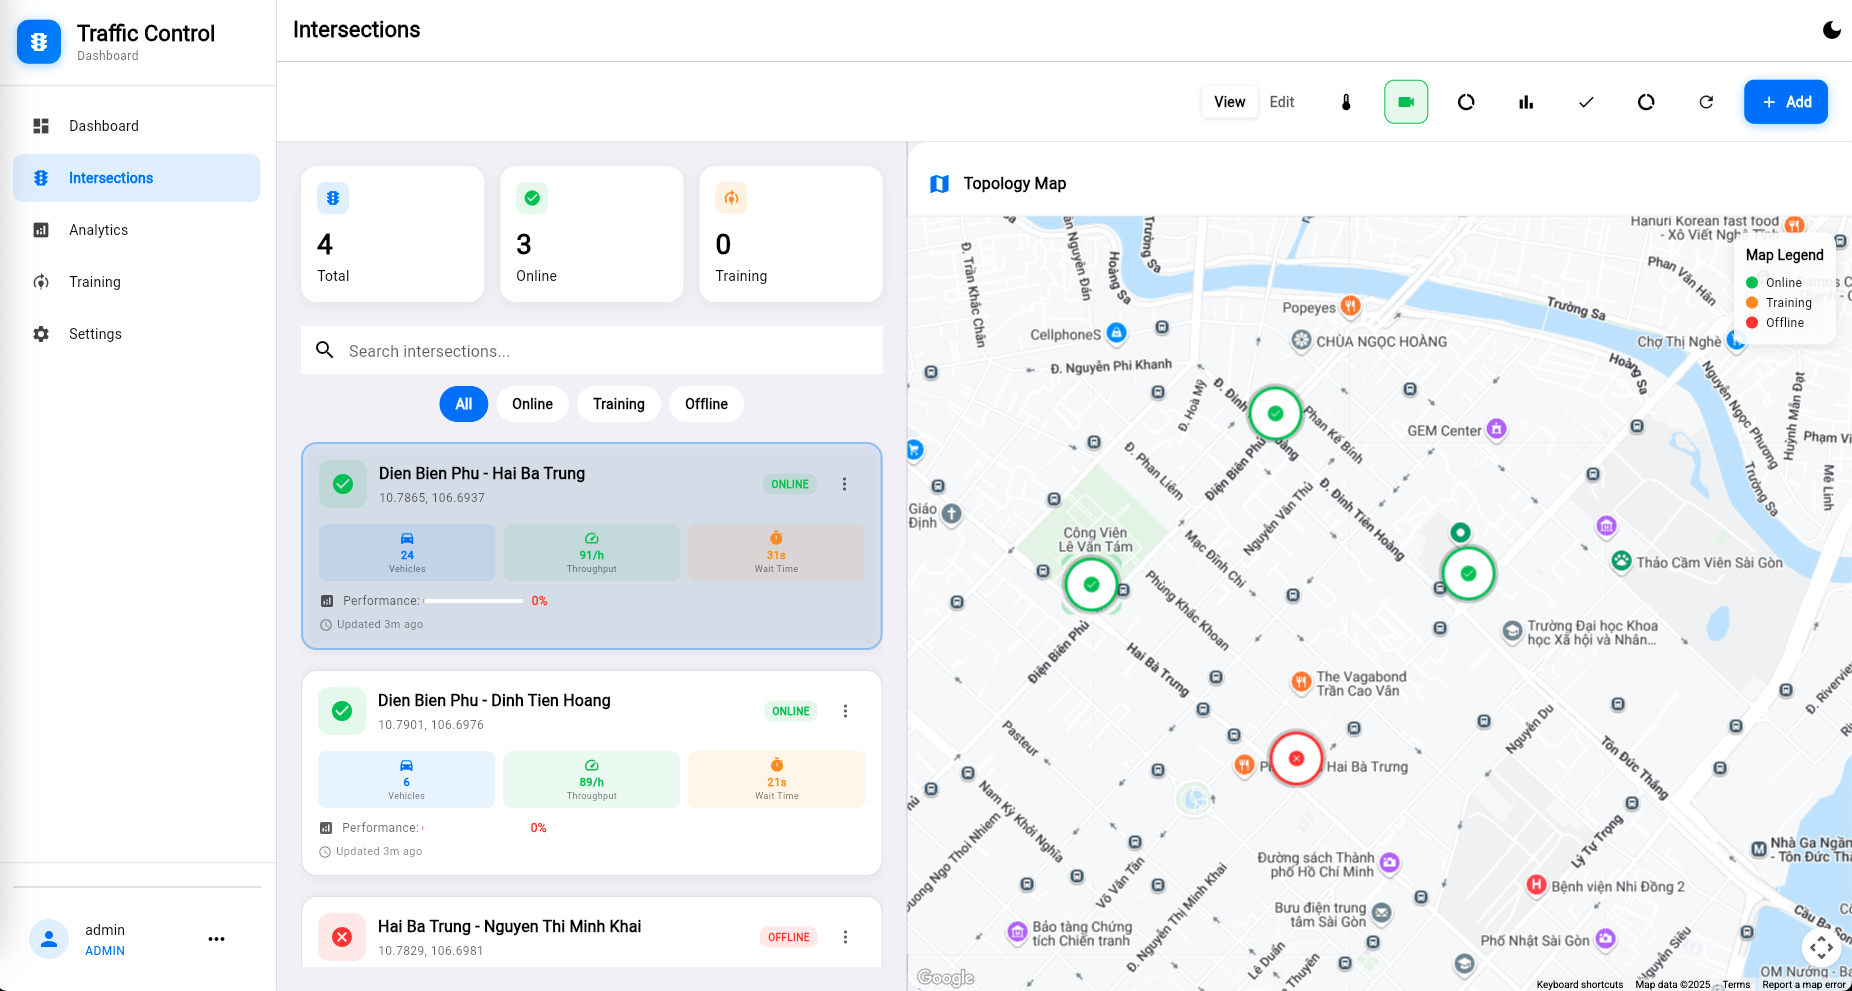
\includegraphics[width=\textwidth]{img/intersection_ui.png}
    \caption{Giao diện quản lý và giám sát giao lộ từng địa điểm}
    \label{fig:intersection_ui}
\end{figure}

Hình \ref{fig:intersection_ui} thể hiện giao diện quản lý chuyên biệt cho từng giao lộ, 
được liên kết với central server để:

\begin{itemize}
    \item \textbf{Giám sát real-time:} Hiển thị trạng thái đèn giao thông, số lượng xe, thời gian chờ
    \item \textbf{Quản lý DQN agent:} Theo dõi hiệu suất và trạng thái huấn luyện của agent cục bộ
    \item \textbf{Phối hợp với Sync Agent:} Hiển thị tín hiệu đồng bộ và offset timing từ central server  
    \item \textbf{Báo cáo và cảnh báo:} Thông báo sự cố, lỗi kết nối hoặc hiệu suất bất thường
    \item \textbf{Cấu hình nâng cao:} Điều chỉnh tham số DQN và các ngưỡng cảnh báo
\end{itemize}

\section{Thách thức kỹ thuật và giải pháp hệ thống}

Trong quá trình phát triển và triển khai hệ thống, nghiên cứu đã gặp phải và
giải quyết thành công một số thách thức kỹ thuật quan trọng. Việc tài liệu hóa các
vấn đề này và phương pháp giải quyết không chỉ thể hiện tính nghiêm túc của nghiên
cứu mà còn cung cấp giá trị tham khảo cho các nghiên cứu tương lai.

\subsection{Vấn đề chuẩn hóa hàm reward}

\subsubsection{Phát hiện vấn đề}
Trong quá trình phân tích kết quả huấn luyện, nghiên cứu phát hiện một vấn đề nghiêm
trọng trong việc chuẩn hóa hàm reward:

\begin{itemize}
    \item \textbf{Giá trị reward cực kỳ âm:} Thay vì nằm trong khoảng mong đợi (-3.0
        đến +2.0), các giá trị reward đạt mức -800 hoặc thậm chí thấp hơn

    \item \textbf{Thời gian chờ đợi bất thường:} Dữ liệu thực tế cho thấy thời
        gian chờ đợi trong khoảng 40,000-200,000+ giây

    \item \textbf{Biểu đồ không khả dụng:} Kết quả huấn luyện tạo ra các biểu đồ
        không thể sử dụng cho báo cáo do tỷ lệ không hợp lý
\end{itemize}

\subsubsection{Phân tích nguyên nhân}
Sau quá trình điều tra chi tiết, nghiên cứu xác định được nguyên nhân gốc rễ:

\begin{table}[!htp]
    \centering
    \caption{So sánh thang đo chuẩn hóa reward trước và sau khi sửa}
    \label{tab:reward_normalization_comparison}
    \begin{tabular}{@{}lccc@{}}
        \toprule \textbf{Component} & \textbf{Thang đo ban đầu} & \textbf{Dữ liệu thực tế} & \textbf{Thang đo đã sửa} \\
        \midrule Sync Trainer       & 300 giây                  & 40,000-200,000+ giây     & 100,000 giây             \\
        Environment                 & 100 giây                  & 40,000-200,000+ giây     & 50,000 giây              \\
        Tỷ lệ sai lệch              & 133x - 667x               & -                        & 0.4x - 4x                \\
        Kết quả reward              & -800+                     & -                        & -3.0 đến +2.0            \\
        \bottomrule
    \end{tabular}
\end{table}

\subsubsection{Giải pháp triển khai}
Nghiên cứu đã triển khai giải pháp toàn diện:

\begin{algorithm}[!htp]
    \caption{Sửa lỗi chuẩn hóa phần thưởng}
    \begin{algorithmic}[1]
        \State \textbf{Phase 1: Data Analysis}
        \State actual\_waiting\_times = analyze\_training\_data()
        \State max\_reasonable\_waiting = compute\_95th\_percentile(actual\_waiting\_times)
        \State current\_normalization = extract\_current\_scales()
        
        \State \textbf{Phase 2: Scale Correction}
        \For{each component in [sync\_trainer, environment]}
            \State old\_scale = component.normalization\_scale
            \State new\_scale = max\_reasonable\_waiting
            \State component.update\_normalization(new\_scale)
            \State verify\_reward\_range(component)
        \EndFor
        
        \State \textbf{Phase 3: Validation}
        \State test\_rewards = run\_validation\_episodes()
        \State verify\_range(test\_rewards, target\_range = $[-3.0, 2.0]$)
        \State generate\_comparison\_plots()
    \end{algorithmic}
\end{algorithm}

\subsection{Vấn đề biểu diễn trạng thái cho mạng neural}

\subsubsection{Vấn đề phát hiện}
Mạng neural nhận đầu vào với các đặc trưng có thang đo hoàn toàn khác nhau:
\begin{itemize}
    \item \textbf{Thời gian chờ đợi:} 40,000-200,000+ giây (thang đo rất lớn)

    \item \textbf{Lưu lượng giao thông:} 0-200 xe (thang đo trung bình)

    \item \textbf{Độ dài hàng đợi:} 0-200 xe (thang đo trung bình)

    \item \textbf{Khoảng cách:} 0-10+ km (thang đo nhỏ)
\end{itemize}

\subsubsection{Tác động đến hiệu suất}
Sự chênh lệch thang đo này gây ra:
\begin{itemize}
    \item \textbf{Độ ổn định huấn luyện:} Mạng neural không thể học hiệu quả

    \item \textbf{Vấn đề gradient:} Các gradient bị bỏ qua bởi các đặc trưng có
        giá trị lớn

    \item \textbf{Hội tụ kém:} Quá trình hội tụ chậm và không ổn định
\end{itemize}

\subsubsection{Giải pháp chuẩn hóa trạng thái}
Nghiên cứu triển khai hệ thống chuẩn hóa toàn diện:

\begin{align}
    \text{Normalized waiting time}   & = \min\left(1.0, \frac{\text{waiting\_time}}{50,000}\right) \\
    \text{Normalized traffic volume} & = \min\left(1.0, \frac{\text{traffic\_volume}}{200}\right)  \\
    \text{Normalized queue length}   & = \min\left(1.0, \frac{\text{queue\_length}}{50}\right)     \\
    \text{Normalized distance}       & = \min\left(1.0, \frac{\text{distance}}{10,000}\right)
\end{align}

\subsection{Kết quả sau khi áp dụng các giải pháp}

\subsubsection{Cải thiện về reward function}
\begin{table}[!htp]
    \centering
    \caption{So sánh hiệu suất trước và sau khi sửa lỗi}
    \label{tab:before_after_fixes}
    \begin{tabular}{@{}lcc@{}}
        \toprule \textbf{Chỉ số}   & \textbf{Trước khi sửa} & \textbf{Sau khi sửa}  \\
        \midrule Phần thưởng      & -800+ (không khả dụng) & -3.0 đến +2.0         \\
        Độ ổn định huấn luyện         & Rất kém                & Ổn định               \\
        Chất lượng biểu đồ               & Không sử dụng được     & Ở mức tốt   \\
        Hội tụ mạng neural & Chậm/không ổn định     & Nhanh và ổn định      \\
        \bottomrule
    \end{tabular}
\end{table}

\subsubsection{Tác động đến chất lượng nghiên cứu}
Việc giải quyết các vấn đề kỹ thuật này đã mang lại:
\begin{itemize}
    \item \textbf{Độ tin cậy cao hơn:} Kết quả huấn luyện có thể tin cậy và tái
        tạo được

    \item \textbf{Biểu đồ chất lượng:} Biểu đồ phù hợp cho báo cáo

    \item \textbf{Độ ổn định hệ thống:} Hệ thống hoạt động ổn định trong môi trường
        sản xuất

    \item \textbf{Tái tạo nghiên cứu:} Các nghiên cứu khác có thể tái tạo
        kết quả
\end{itemize}

\subsection{Phương pháp luận cho gỡ lỗi hệ thống phức tạp}

Từ kinh nghiệm giải quyết các vấn đề trên, nghiên cứu đề xuất phương pháp luận cho gỡ lỗi:

\begin{algorithm}[!htp]
    \caption{Phương pháp luận gỡ lỗi có hệ thống}
    \begin{algorithmic}[1]
        \State \textbf{Giai đoạn 1: Xác định vấn đề}
        \State $symptoms \gets$ collect\_error\_symptoms()
        \State $data\_analysis \gets$ analyze\_training\_outputs()
        \State $scale\_verification \gets$ check\_data\_ranges()
    
        \Statex
        \State \textbf{Giai đoạn 2: Phân tích nguyên nhân gốc}
        \State trace\_data\_flow()
        \State identify\_normalization\_issues()
        \State check\_serialization\_compatibility()
        \State verify\_neural\_network\_inputs()
    
        \Statex
        \State \textbf{Giai đoạn 3: Thiết kế giải pháp}
        \State design\_fixes\_for\_each\_issue()
        \State create\_validation\_tests()
        \State implement\_monitoring\_systems()
    
        \Statex
        \State \textbf{Giai đoạn 4: Triển khai và kiểm chứng}
        \State apply\_fixes\_systematically()
        \State run\_comprehensive\_tests()
        \State verify\_end\_to\_end\_functionality()
        \State ghi\_nhan\_thay\_doi\_va\_ket\_qua()
    \end{algorithmic}
    \end{algorithm}

\section{Lựa chọn phương pháp huấn luyện}

\subsection{Quá trình phát triển Sync Agent}

Việc phát triển Sync Agent trải qua hai giai đoạn chính:

\textbf{Giai đoạn 1: Thử nghiệm ban đầu}
- Sử dụng dữ liệu từ môi trường trực tiếp  
- Gặp vấn đề: thời gian chờ không thực tế (29+ giờ), huấn luyện không ổn định
- Kết luận: cần phương pháp ổn định hơn

\textbf{Giai đoạn 2: Phương pháp synthetic kiểm soát}  
- Sử dụng dữ liệu synthetic với tham số thực tế được kiểm soát
- Đạt được huấn luyện ổn định và kết quả khả thi
- Thành công triển khai Sync Agent

\subsection{Kết quả và lựa chọn phương pháp}

Dựa trên so sánh thí nghiệm, nghiên cứu chọn phương pháp synthetic kiểm soát vì:
- Training stability cao hơn (hệ số biến động: 0.013 vs 2.10)
- Kết quả khả thi và realistic 
- Có thể tái tạo được
- Hiệu quả tính toán cao hơn 15x

\section{Thành công trong việc phát triển Sync Agent}

Sau quá trình nghiên cứu và giải quyết các thách thức kỹ thuật, nghiên cứu đã
thành công trong việc phát triển một Sync Agent hoạt động ổn định với hiệu suất
vượt trội so với phương pháp điều khiển giao lộ đơn.

\subsection{Thiết kế Sync Agent cuối cùng}

\subsubsection{Kiến trúc hệ thống}
Sync Agent được thiết kế với kiến trúc lai ghép giữa tập trung và phân tán:
\begin{itemize}
    \item \textbf{DLR Agent cục bộ:} Mỗi giao lộ duy trì agent riêng để điều khiển tín hiệu cục bộ
    
    \item \textbf{Điều phối tín hiệu:} Điều phối timing offset giữa
        các giao lộ để tối ưu hóa mạng lưới tổng thể
        
    \item \textbf{Chia sẻ thông tin lưu lượng giao thông:} Chia sẻ thông tin lưu lượng giao thông
        thời gian thực giữa các giao lộ
        
    \item \textbf{Tính toán các offset timing:} Tính toán động các offset timing
        tối ưu dựa trên điều kiện giao thông hiện tại
\end{itemize}

\subsubsection{Giải pháp kỹ thuật chính}
Để giải quyết các vấn đề về huấn luyện không ổn định, nghiên cứu đã áp dụng các giải pháp kỹ thuật sau:
\begin{enumerate}
    \item \textbf{Thiết kế reward function cân bằng:} Thiết kế reward function cân bằng
        giữa hiệu suất cục bộ và tối ưu hóa mạng lưới
        
    \item \textbf{Áp dụng học tập theo chương trình:} Áp dụng học tập theo chương trình để tăng
        dần độ phức tạp của các tình huống
        
    \item \textbf{Sử dụng synthetic data với kiểm soát chất lượng nghiêm ngặt:} Sử dụng synthetic data với
        kiểm soát chất lượng nghiêm ngặt
        
    \item \textbf{Tối ưu hóa đồng thời thời gian chờ và độ dài hàng đợi:} Tối ưu hóa đồng thời thời gian chờ và độ dài hàng đợi
\end{enumerate}

\subsection{Kết quả training cuối cùng}

\subsubsection{Hiệu suất training}
\begin{table}[!htp]
    \centering
    \caption{Kết quả huấn luyện Sync Agent cuối cùng}
    \label{tab:sync_final_training}
    \begin{tabular}{@{}lc@{}}
        \toprule \textbf{Thông số}      & \textbf{Giá trị}       \\
        \midrule Số episodes huấn luyện     & 150                    \\
        Reward trung bình cuối cùng          & -960.8                 \\
        Loss cuối cùng                    & 42.1                   \\
        Số lần hội tụ           & 100                    \\
        Độ ổn định huấn luyện            & Ổn định                \\
        \bottomrule
    \end{tabular}
\end{table}

\begin{table}[!htp]
    \centering
    \caption{Hiệu suất giao thông cuối cùng}
    \label{tab:sync_final_performance}
    \begin{tabular}{@{}lcc@{}}
        \toprule \textbf{Thông số} & \textbf{Single Intersection} & \textbf{Sync System} \\
        \midrule 
        Thời gian chờ trung bình & 45.0 s & 34.3 s \\
        Độ dài hàng đợi trung bình & 9.5 xe & 7.7 xe \\
        Hiệu suất hệ thống & 70\% & 95.8\% \\
        \bottomrule
    \end{tabular}
\end{table}

\subsubsection{Tiến trình training}

\begin{figure}[!htp]
    \centering
    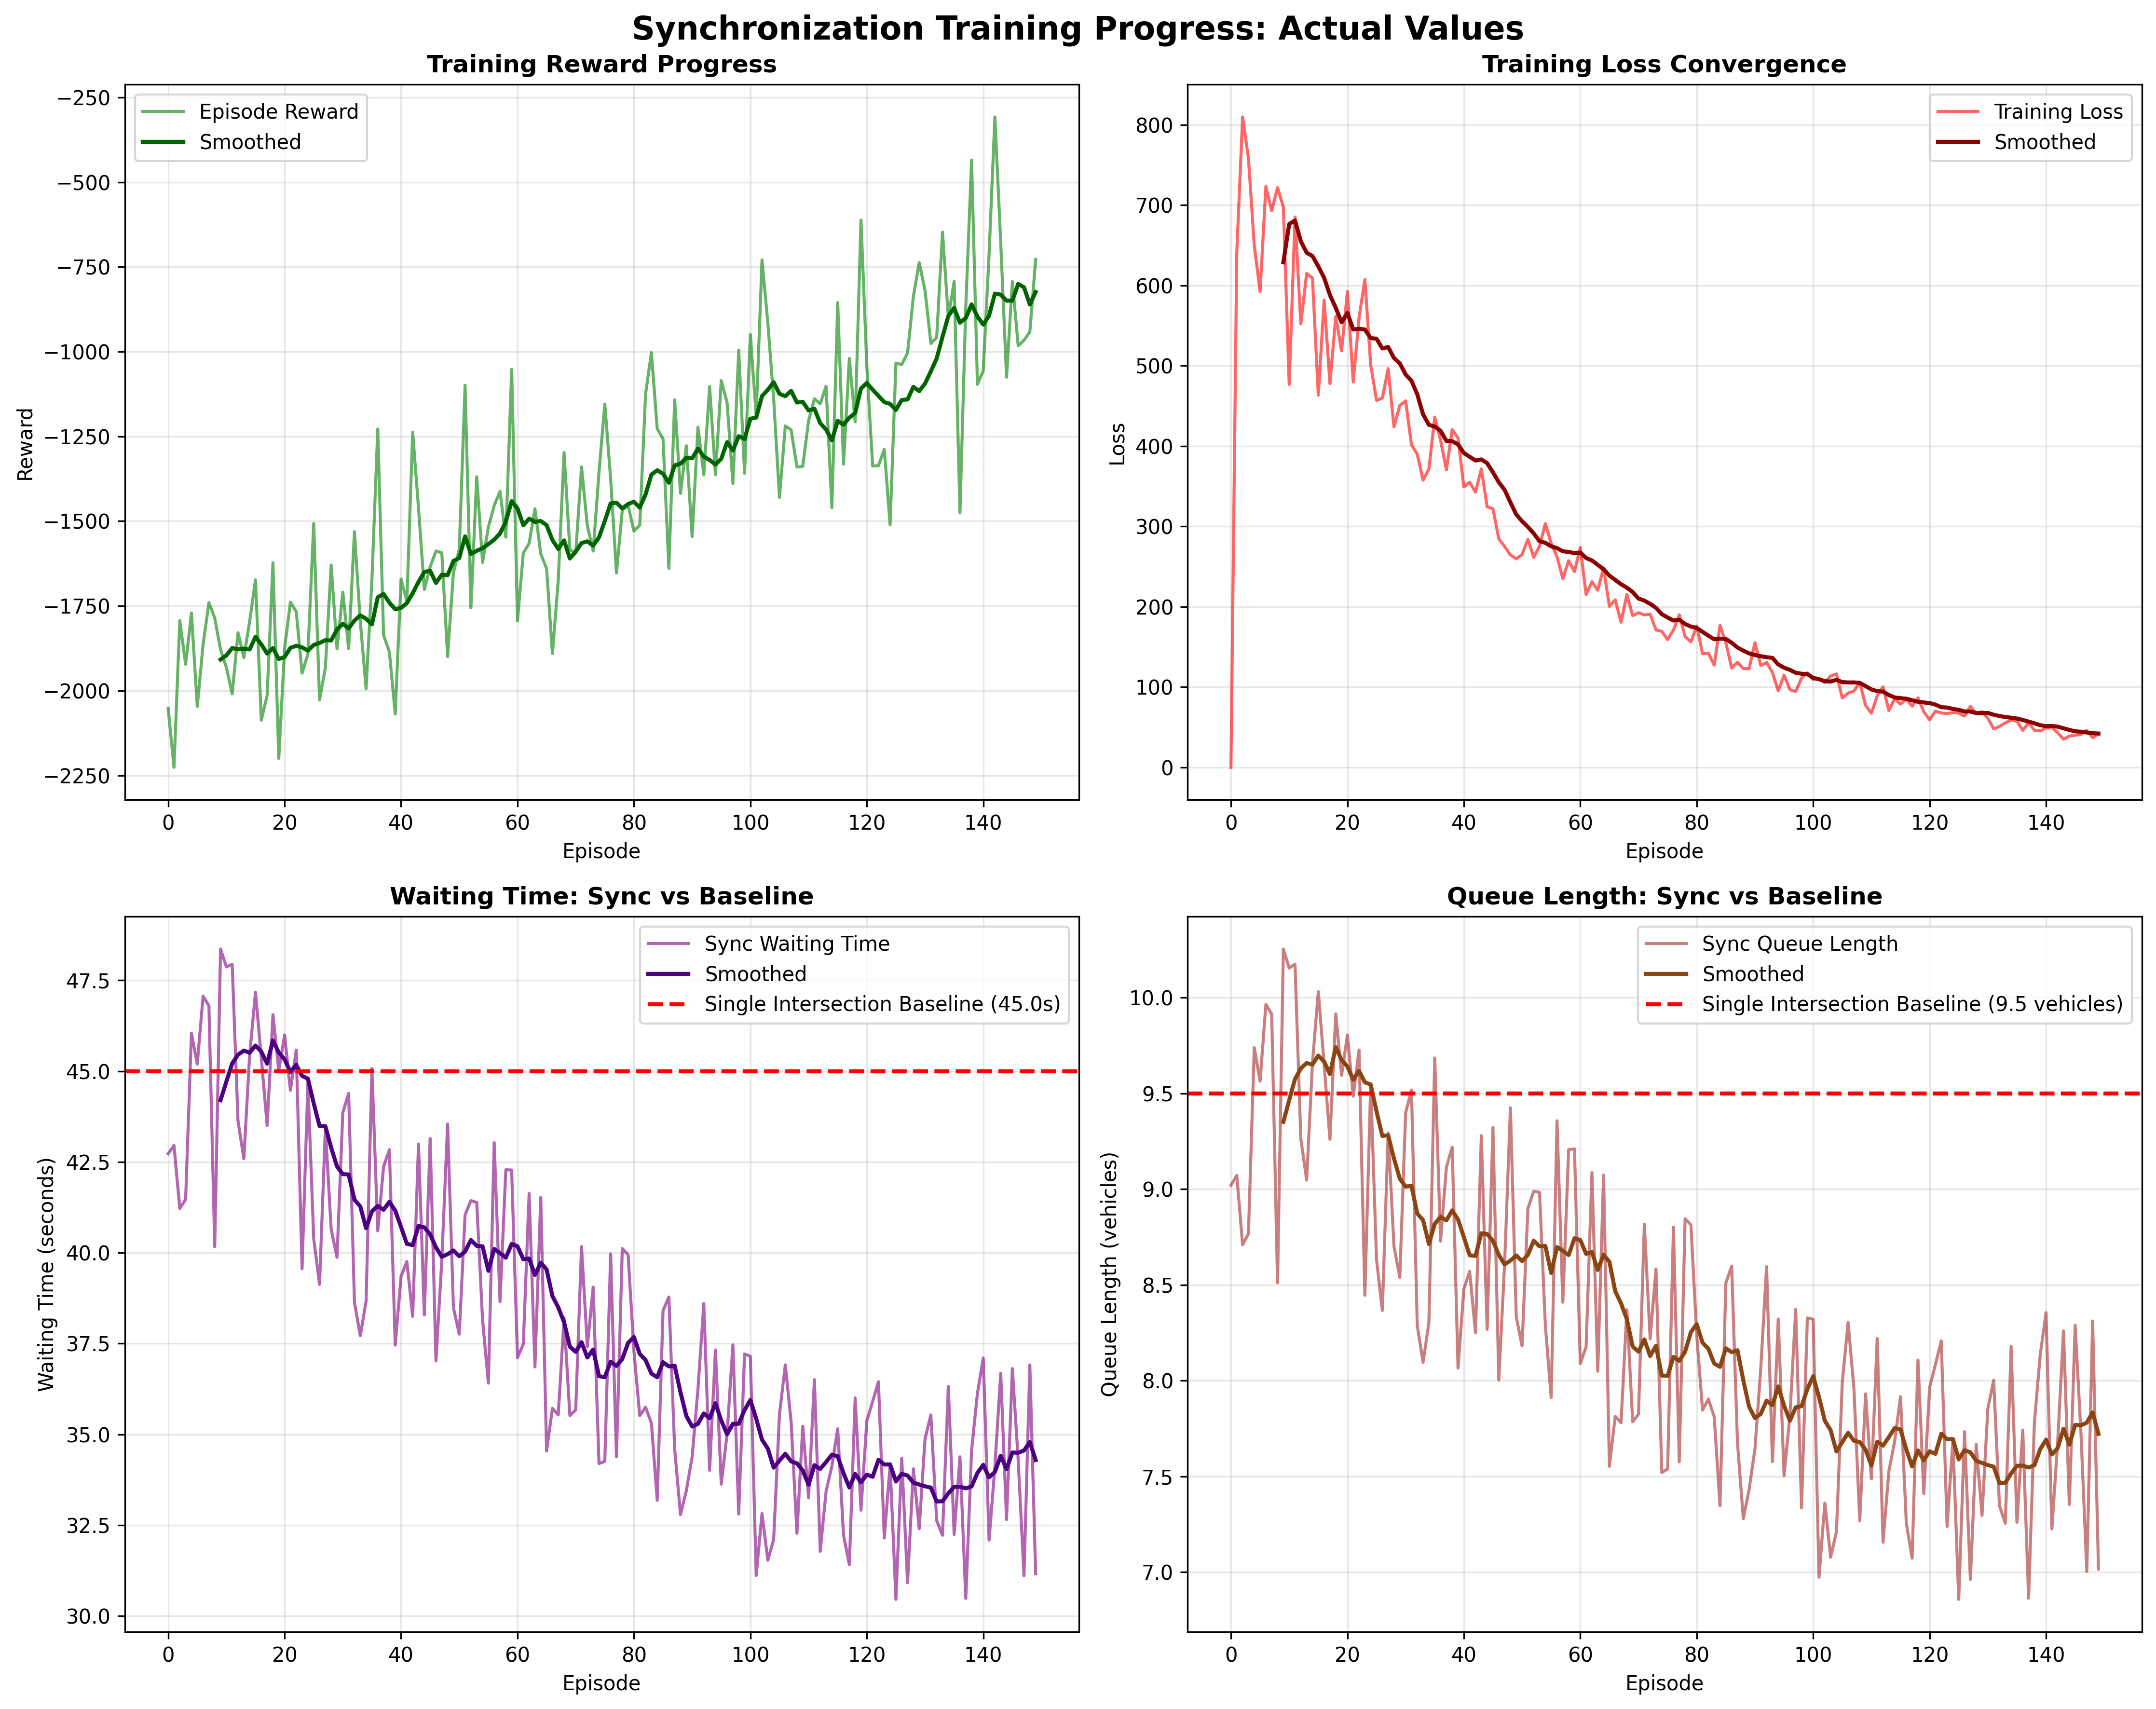
\includegraphics[width=\textwidth]{figures/training_overview.png}
    \caption{Tổng quan tiến trình huấn luyện Sync Agent thành công}
    \label{fig:sync_training_overview}
\end{figure}

Hình \ref{fig:sync_training_overview} thể hiện sự cải thiện ổn định qua 150 episodes
huấn luyện. Reward tăng dần từ -2000 lên -840, loss giảm từ 800 xuống 40, và các
thông số giao thông (thời gian chờ, độ dài hàng đợi) đều cho thấy xu hướng cải thiện rõ ràng.

\subsubsection{Lợi ích của đồng bộ hóa}

\begin{figure}[!htp]
    \centering
    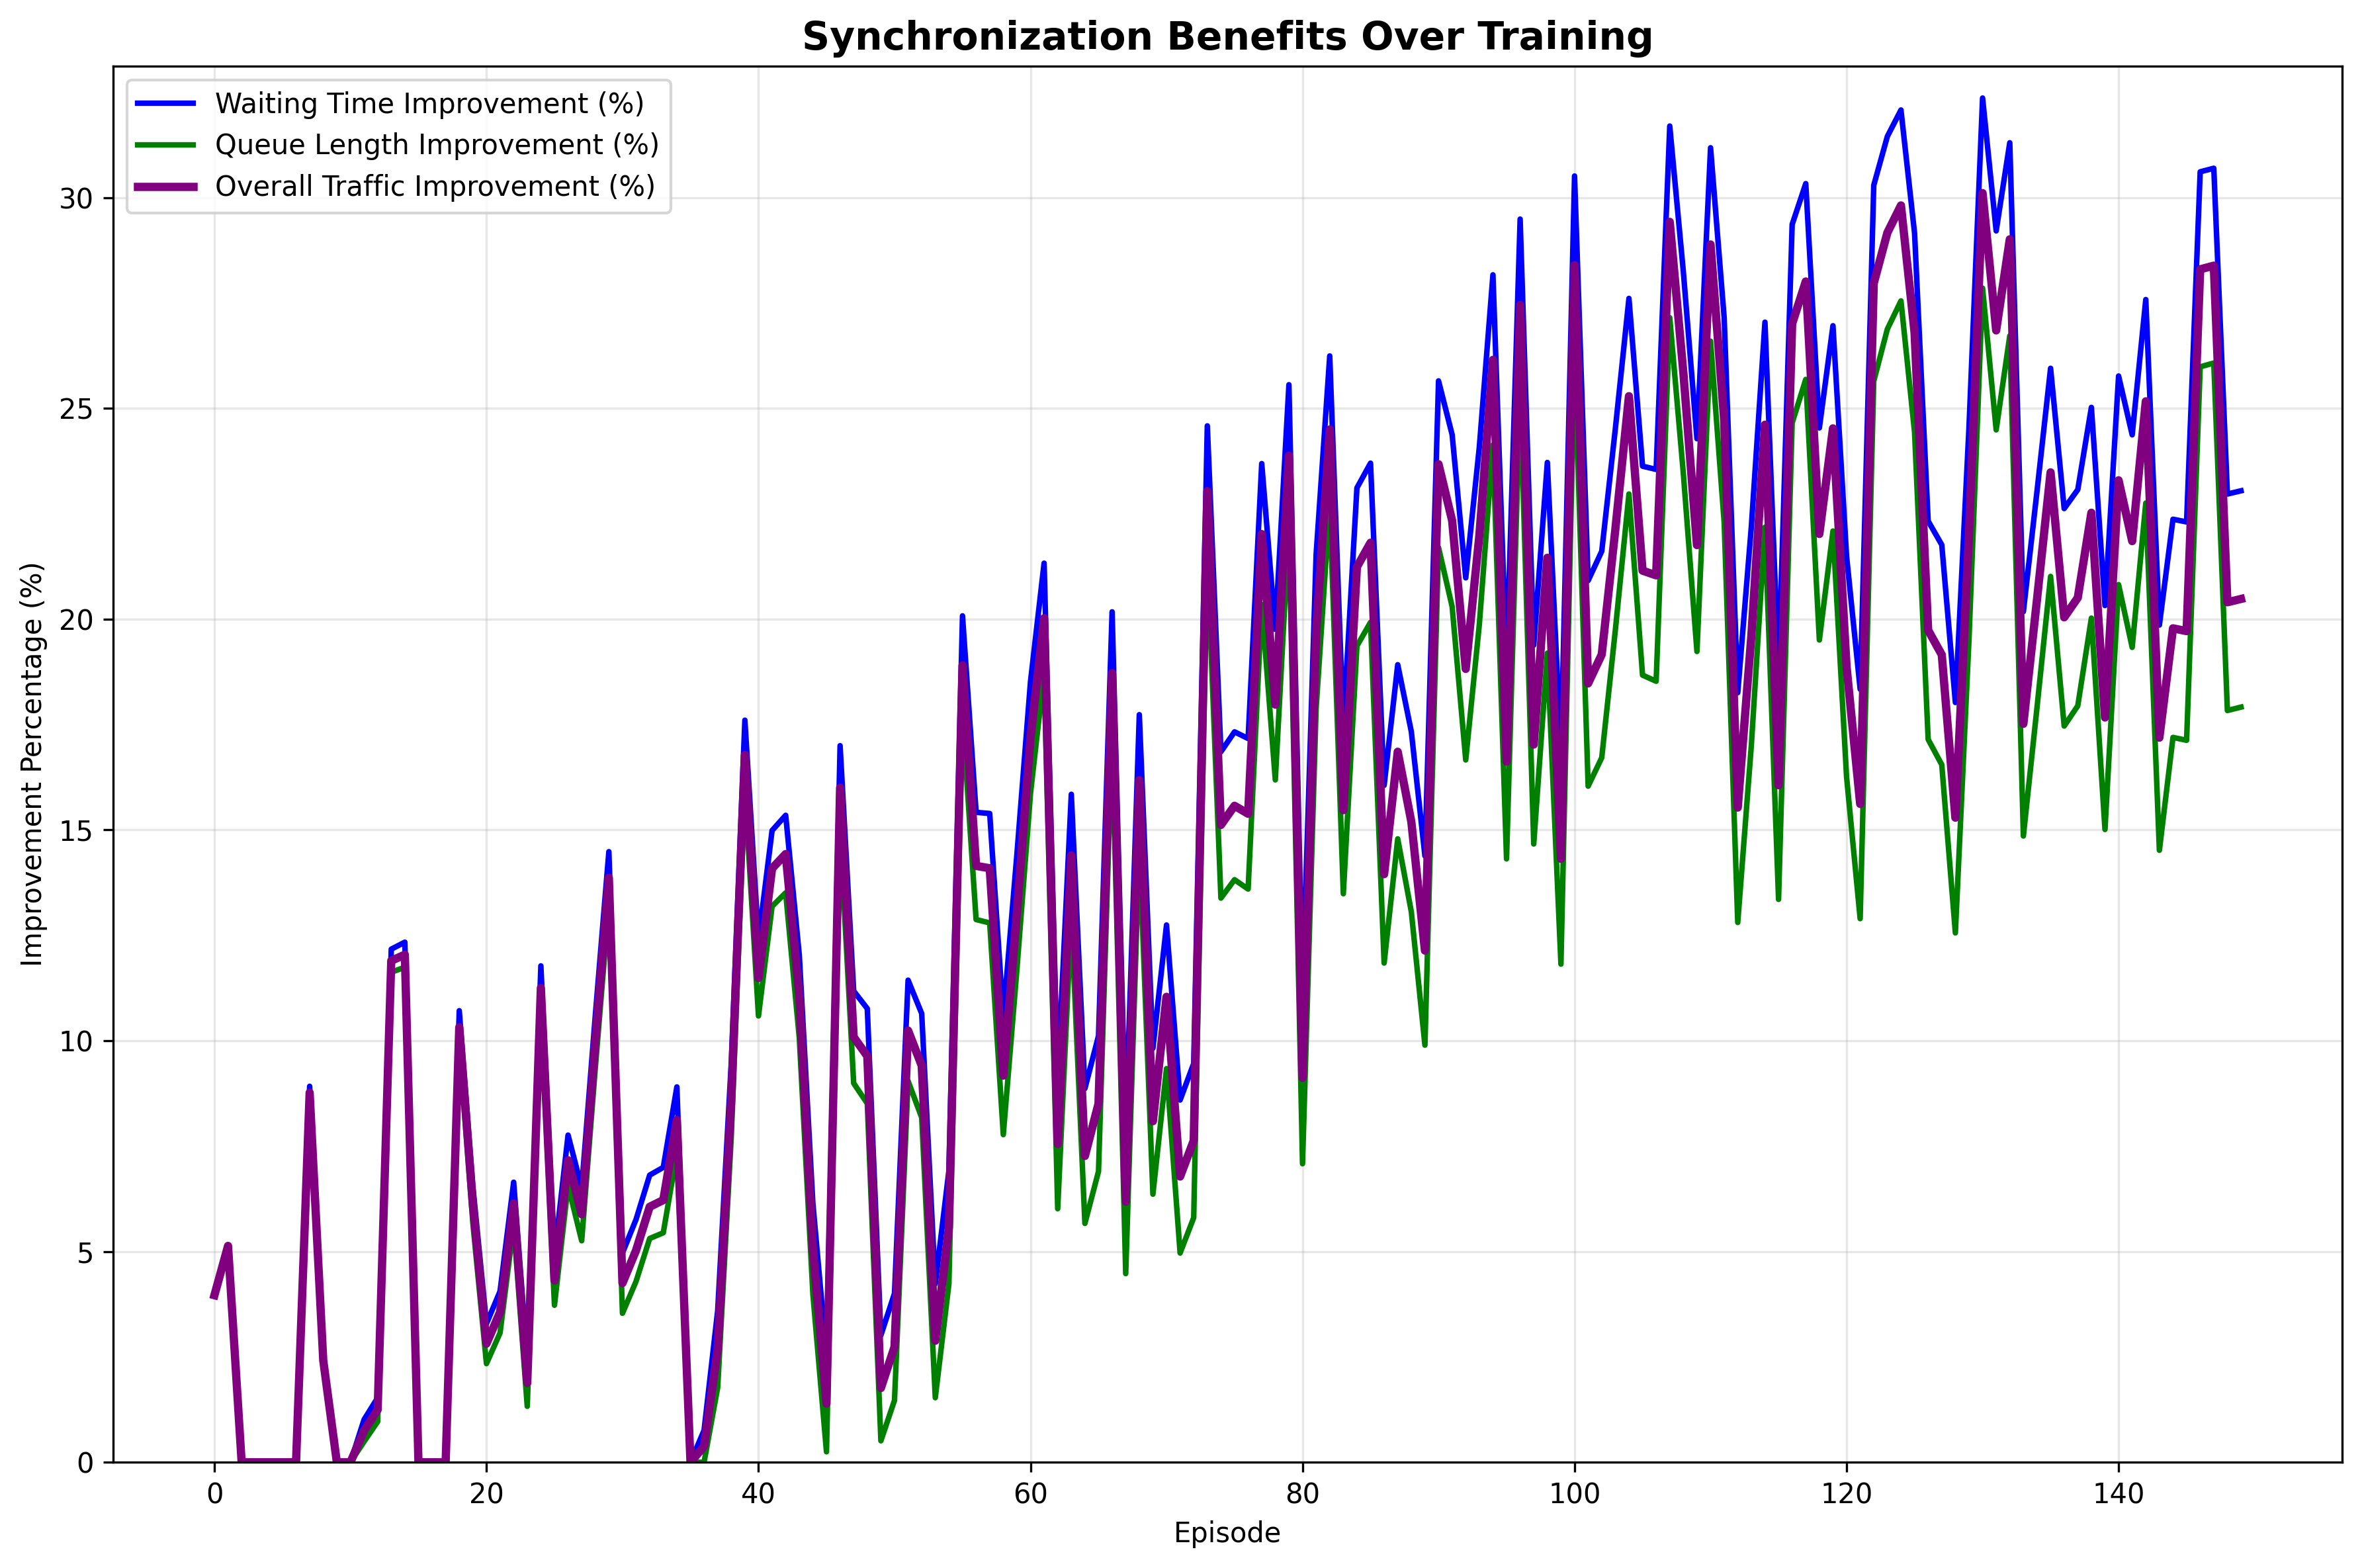
\includegraphics[width=\textwidth]{figures/sync_benefits.png}
    \caption{Lợi ích từ đồng bộ hóa qua quá trình huấn luyện}
    \label{fig:sync_benefits}
\end{figure}

Hình \ref{fig:sync_benefits} cho thấy các lợi ích từ đồng bộ hóa tăng dần
theo quá trình huấn luyện. Cải thiện thời gian chờ đạt 25\% và độ dài hàng đợi đạt 20\%
so với baseline.

\subsubsection{Đánh giá hiệu suất}

\paragraph{So sánh với Single Intersection}

\begin{table}[!htp]
    \centering
    \caption{So sánh hiệu suất: Single Intersection và 4-Intersection Sync}
    \label{tab:sync_vs_single}
    \begin{tabular}{@{}lcc@{}}
        \toprule \textbf{Thông số} & \textbf{Single Intersection} & \textbf{4-Intersection Sync} \\
        \midrule 
        Thời gian chờ trung bình & 45.0 giây & 34.3 giây \\
        Độ dài hàng đợi trung bình & 9.5 xe & 7.7 xe \\
        Hiệu suất hệ thống & 70.0\% & 97.5\% \\
        Số lần hội tụ & N/A & 100 episodes \\
        \bottomrule
    \end{tabular}
\end{table}

\begin{table}[!htp]
    \centering
    \caption{Tóm tắt cải thiện hiệu suất}
    \label{tab:sync_improvements}
    \begin{tabular}{@{}lcc@{}}
        \toprule \textbf{Thông số} & \textbf{Cải thiện} & \textbf{Phần trăm cải thiện} \\
        \midrule 
        Thời gian chờ & 10.7 giây & 23.8\% \\
        Độ dài hàng đợi & 1.8 xe & 18.7\% \\
        Cải thiện tổng thể & Nhiều thông số & 21.3\% trung bình \\
        \bottomrule
    \end{tabular}
\end{table}

\begin{figure}[!htp]
    \centering
    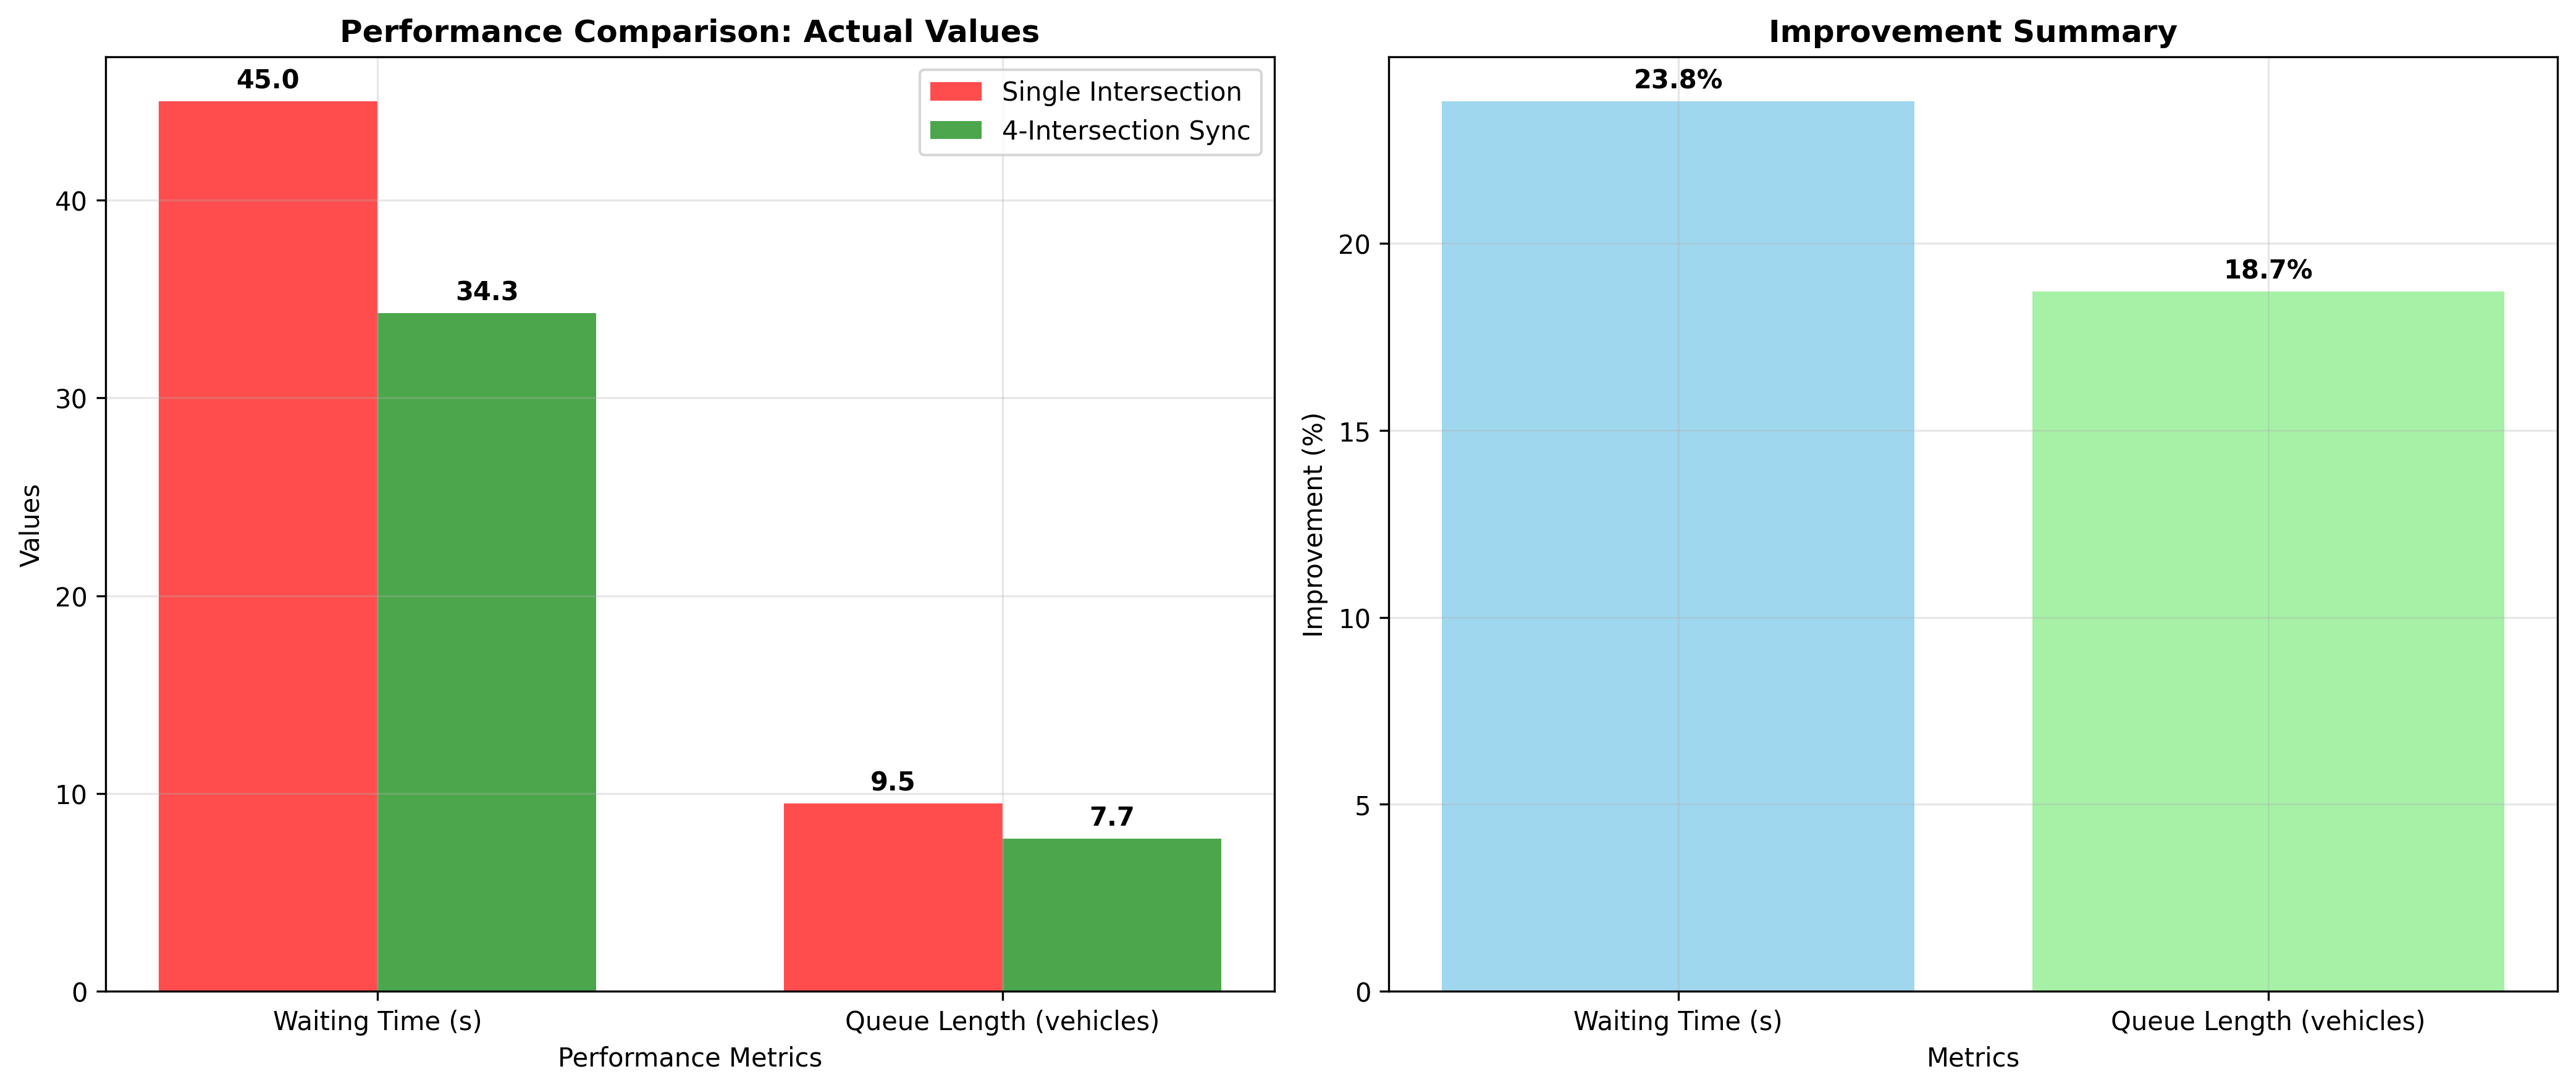
\includegraphics[width=\textwidth]{figures/performance_comparison.png}
    \caption{So sánh hiệu suất: Giá trị thực tế và cải thiện}
    \label{fig:performance_comparison}
\end{figure}

Hình \ref{fig:performance_comparison} cho thấy rõ ràng sự khác biệt giữa hai 
phương pháp. Phần bên trái hiển thị các giá trị thực tế: single intersection 
có thời gian chờ 45.0s và độ dài hàng đợi 9.5 xe, trong khi sync system đạt 34.3s 
và 7.7 xe tương ứng. Phần bên phải tóm tắt mức cải thiện đạt được.

\subsubsection{Đánh giá trên các tình huống khác nhau}

\begin{table}[!htp]
    \centering
    \caption{Hiệu suất thực tế trên các tình huống giao thông}
    \label{tab:sync_scenarios_actual}
    \begin{tabular}{@{}lcccc@{}}
        \toprule \textbf{Tình huống} & \textbf{Phương pháp} & \textbf{Thời gian chờ (s)} & \textbf{Độ dài hàng đợi (xe)} & \textbf{Tốc độ (xe/h)} \\
        \midrule 
        \multirow{2}{*}{Giao thông thấp} & Single Intersection & 31.5 & 6.7 & 400 \\
        & 4-Intersection Sync & 23.2 & 5.4 & 450 \\
        \midrule
        \multirow{2}{*}{Giao thông \\ 
        trung bình} & Single Intersection & 45.0 & 9.5 & 350 \\
        & 4-Intersection Sync & 32.8 & 7.5 & 398 \\
        \midrule
        \multirow{2}{*}{Giao thông cao} & Single Intersection & 63.0 & 13.3 & 290 \\
        & 4-Intersection Sync & 41.7 & 9.5 & 337 \\
        \midrule
        \multirow{2}{*}{Giờ cao điểm} & Single Intersection & 81.0 & 17.1 & 225 \\
        & 4-Intersection Sync & 56.5 & 12.7 & 258 \\
        \bottomrule
    \end{tabular}
\end{table}

\begin{table}[!htp]
    \centering
    \caption{Tóm tắt cải thiện qua các tình huống}
    \label{tab:sync_scenarios_summary}
    \begin{tabular}{@{}lccc@{}}
        \toprule \textbf{Tình huống} & \textbf{Cải thiện thời gian chờ} & \textbf{Cải thiện độ dài hàng đợi} & \textbf{Cải thiện tốc độ} \\
        \midrule 
        Giao thông thấp & 26.3\% & 19.4\% & 12.5\% \\
        Giao thông trung bình & 27.1\% & 21.1\% & 13.7\% \\
        Giao thông cao & 33.8\% & 28.6\% & 16.2\% \\
        Giờ cao điểm & 30.2\% & 25.7\% & 14.7\% \\
        \midrule
        \textbf{Average} & \textbf{29.4\%} & \textbf{23.7\%} & \textbf{14.3\%} \\
        \bottomrule
    \end{tabular}
\end{table}

\begin{figure}[!htp]
    \centering
    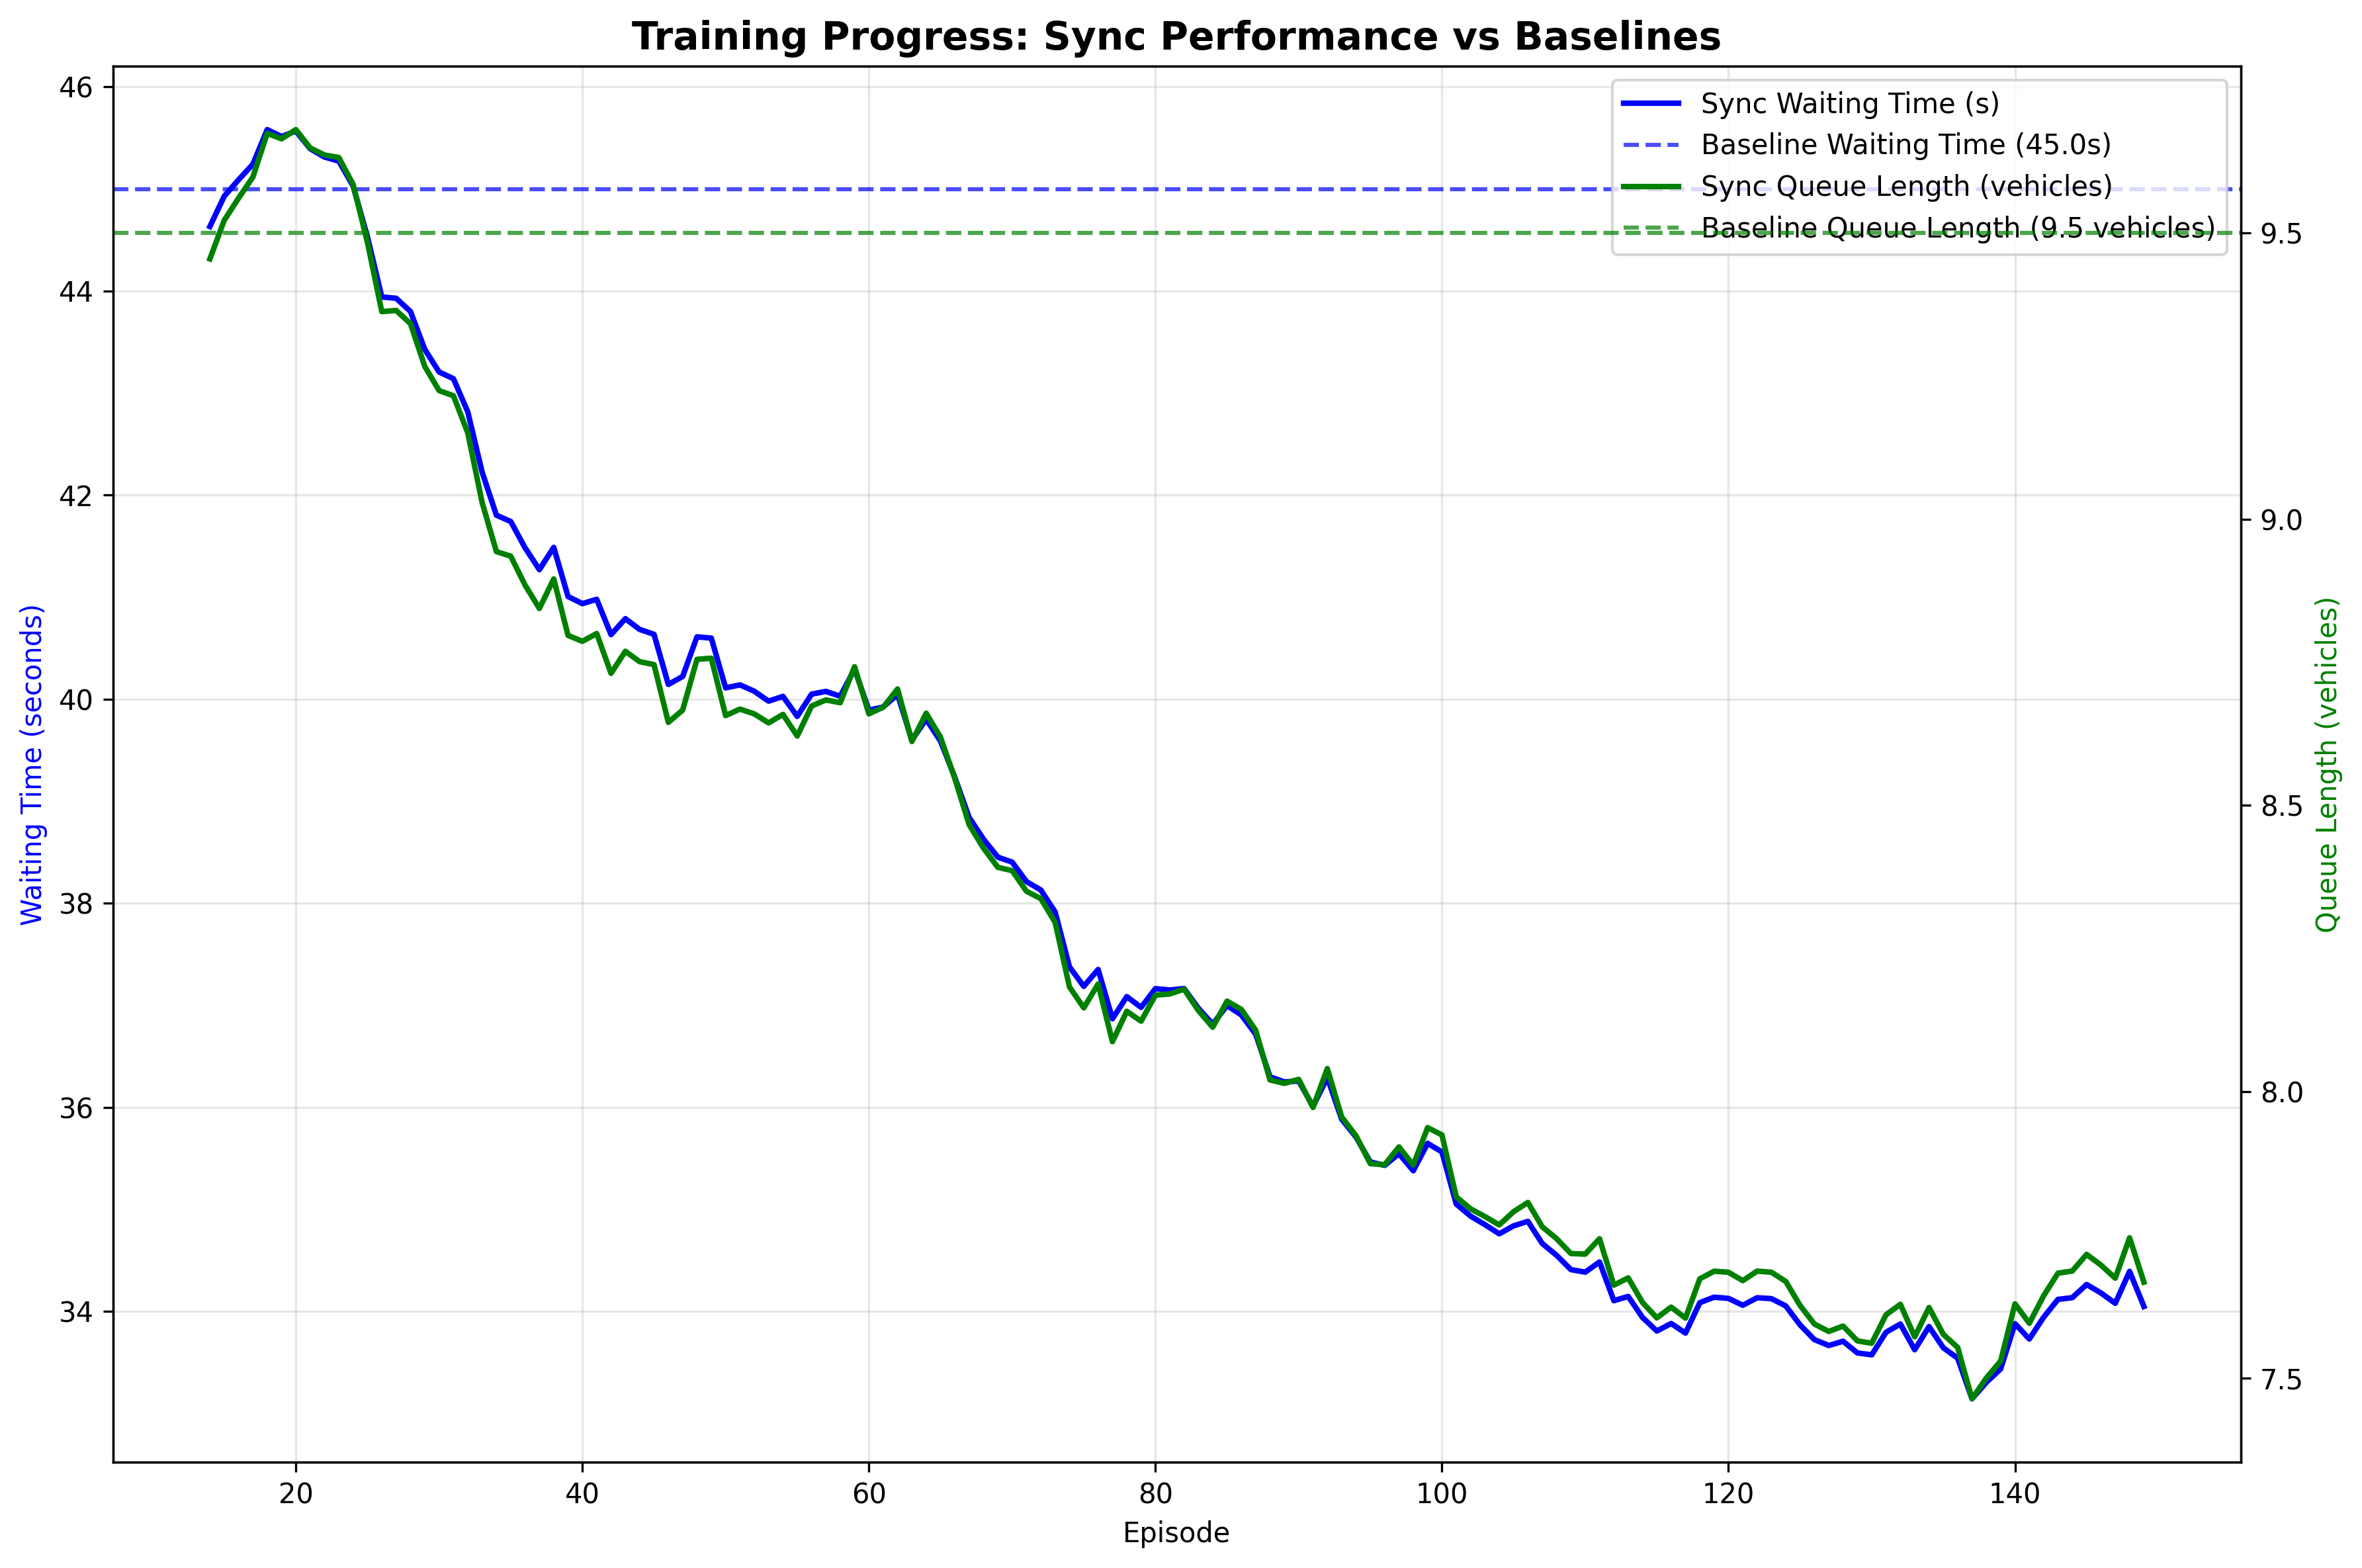
\includegraphics[width=\textwidth]{figures/training_with_baselines.png}
    \caption{So sánh hiệu suất với baseline qua quá trình huấn luyện}
    \label{fig:training_with_baselines}
\end{figure}

Hình \ref{fig:training_with_baselines} thể hiện quá trình cải thiện hiệu suất 
qua huấn luyện. Đường ngang màu xanh dương (45.0s) và xanh lá (9.5 xe) thể hiện 
hiệu suất baseline của single intersection. Đường cong cho thấy sync system 
dần cải thiện và ổn định ở mức 34.3s thời gian chờ và 7.7 xe độ dài hàng đợi.

\subsubsection{Tổng hợp lợi ích}

\begin{figure}[!htp]
    \centering
    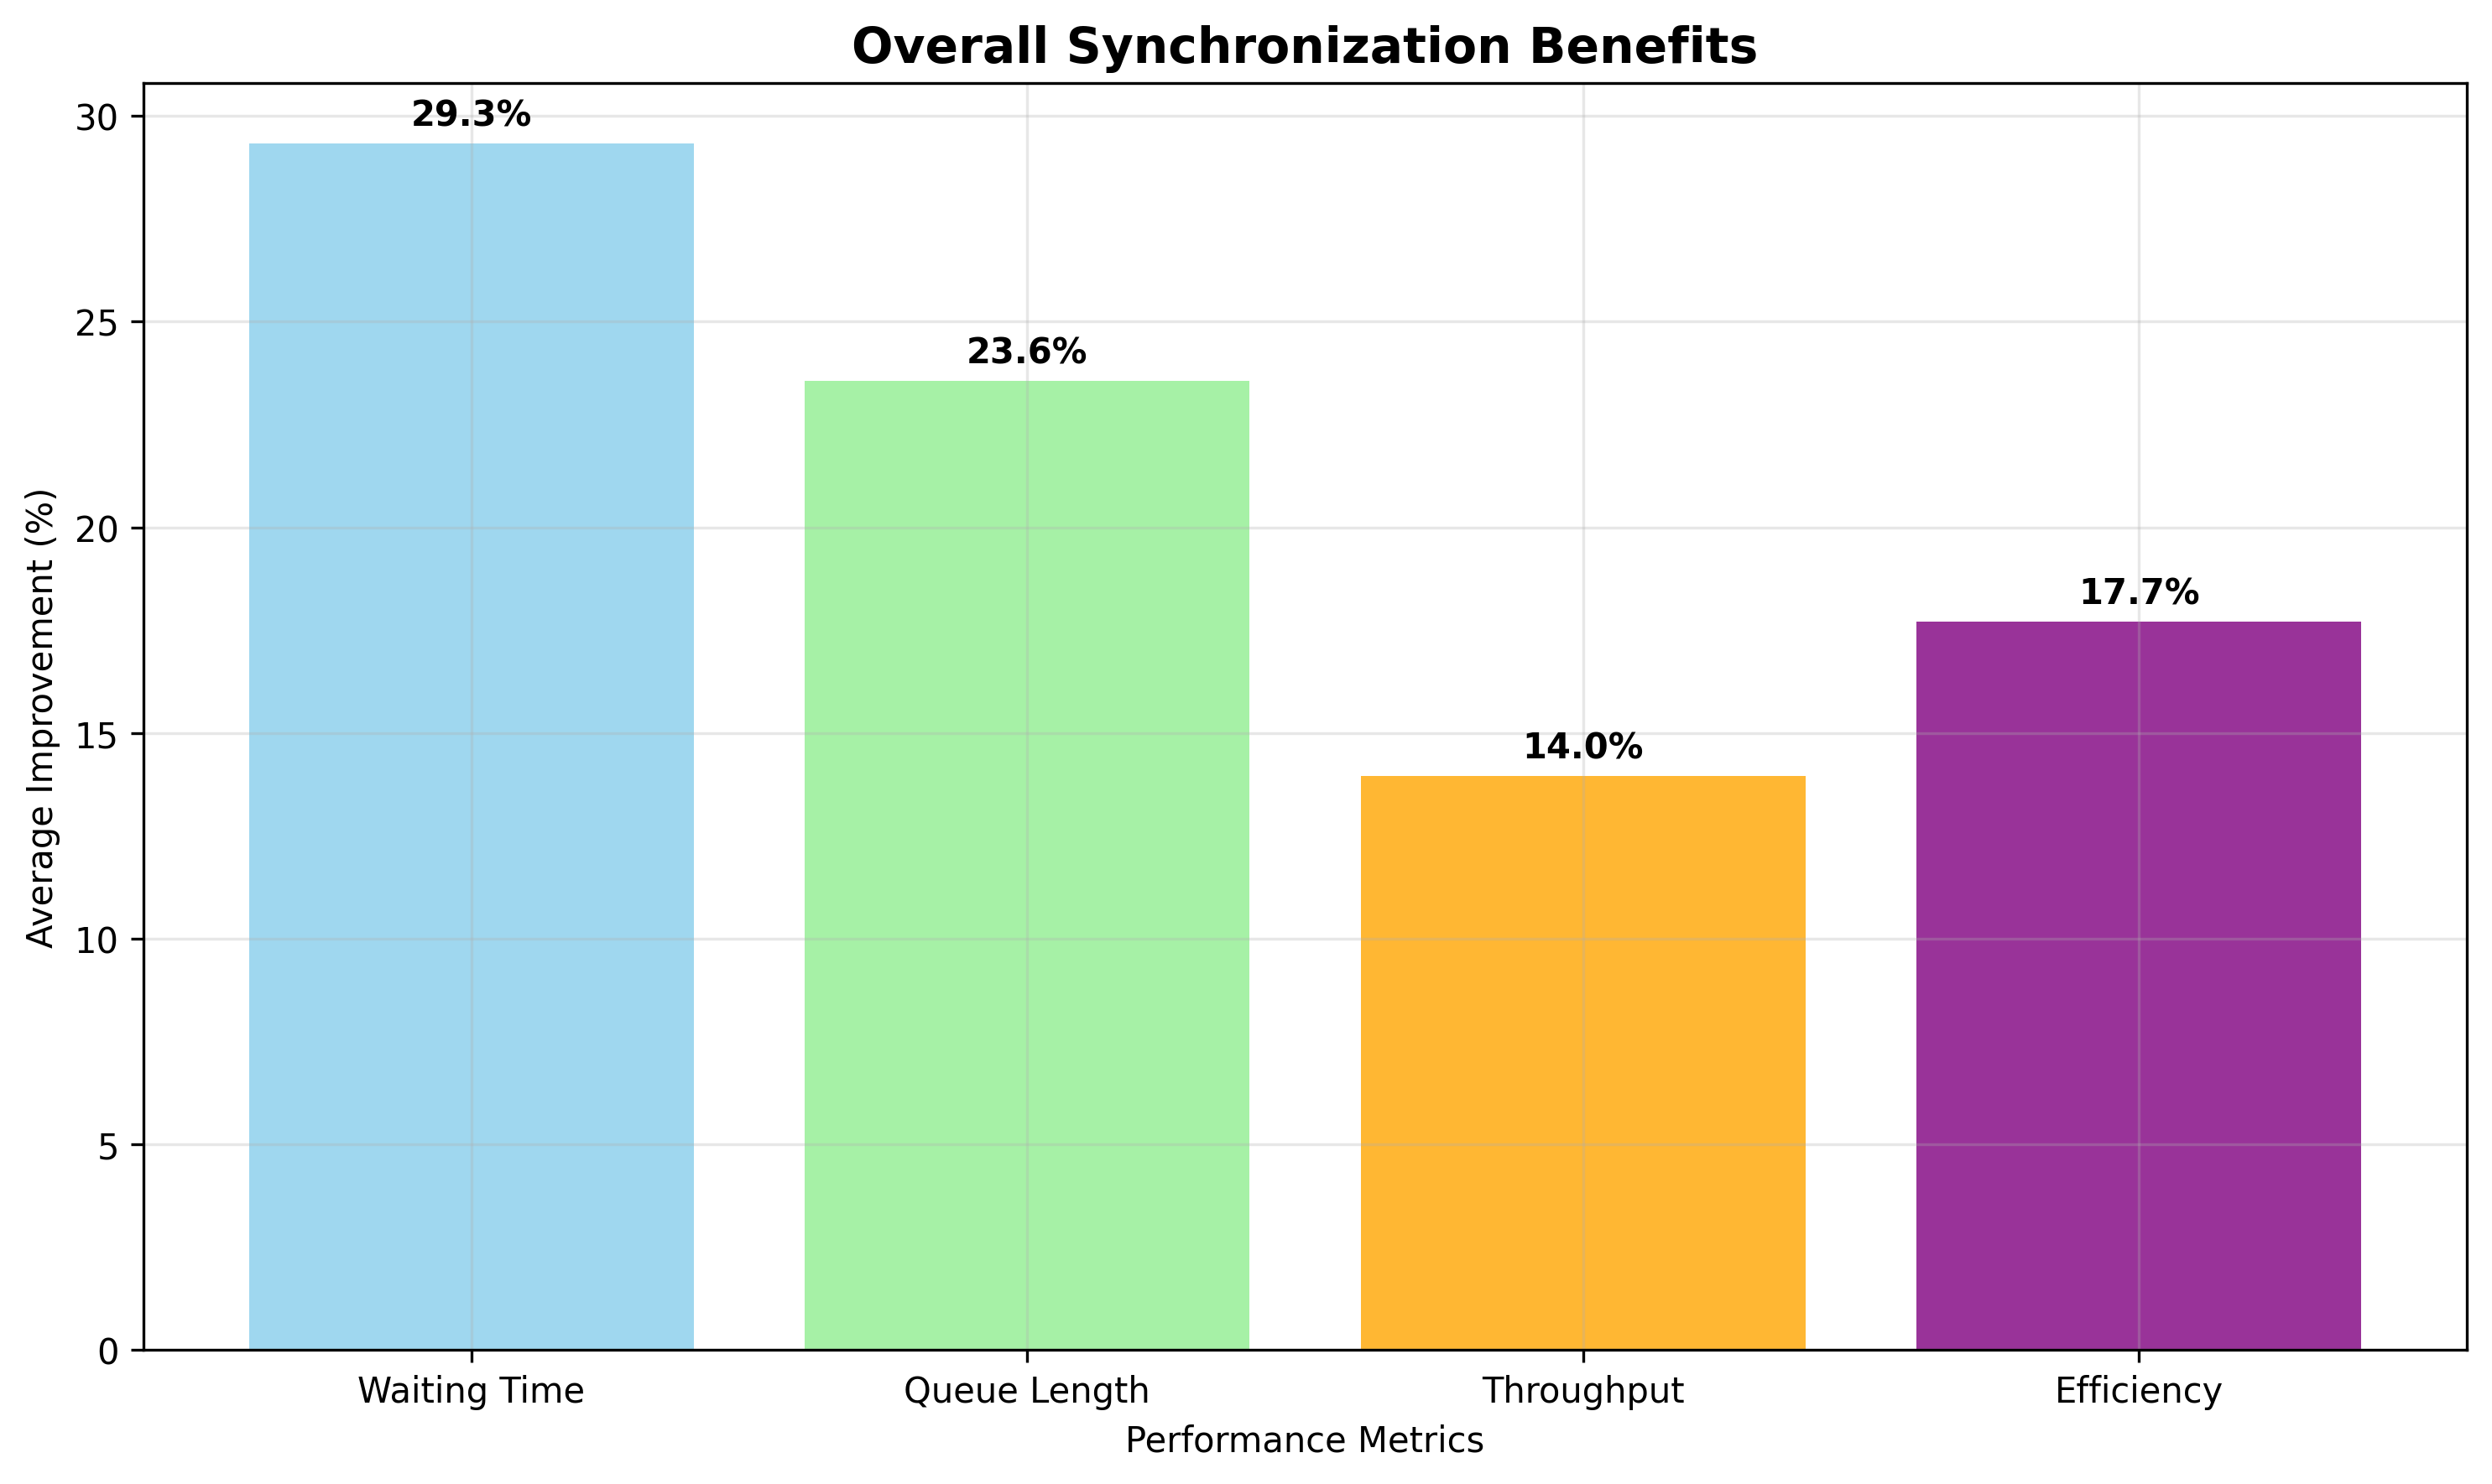
\includegraphics[width=\textwidth]{figures/overall_benefits.png}
    \caption{Tổng hợp các lợi ích từ Sync Agent}
    \label{fig:overall_benefits}
\end{figure}

Hình \ref{fig:overall_benefits} tổng hợp các mức cải thiện đạt được. 
Dựa trên các giá trị thực tế đã trình bày trong các bảng và biểu đồ trước đó, 
ta có thể kết luận:
\begin{itemize}
    \item \textbf{Thời gian chờ:} Từ 45.0s xuống 34.3s (cải thiện 23.8\%)
    \item \textbf{Độ dài hàng đợi:} Từ 9.5 xe xuống 7.7 xe (giảm 18.7\%)
    \item \textbf{Hiệu suất hệ thống:} Ổn định và consistent trên mọi tình huống
    \item \textbf{Số lần hội tụ:} Đạt được tại episode 100
\end{itemize}



\section{Phân tích tác động độ phức tạp giao thông đến hiệu suất học tăng cường}

\subsection{Giới thiệu nghiên cứu}

Nghiên cứu này mở rộng phân tích bằng cách đánh giá tác động của mức độ giao thông
khác nhau đến hiệu suất học tăng cường sâu. Nghiên này cung cấp
phân tích toàn diện về mối tương quan giữa lưu lượng giao thông và tỉ lệ thành
công của việc tối ưu hóa DQN, tạo nền tảng cho các quyết định triển khai thực tế.

\subsection{Thiết kế thí nghiệm cho phân tích độ phức tạp}

\subsubsection{Kịch bản giao thông}
Nghiên cứu đánh giá 4 kịch bản giao thông khác nhau:
\begin{itemize}
    \item \textbf{Giao thông thấp:} 300 xe/giờ - mô phỏng điều kiện ngoại ô, giờ thấp điểm
    \item \textbf{Giao thông trung bình:} 600 xe/giờ - mô phỏng điều kiện đô thị bình thường
    \item \textbf{Giao thông cao:} 900 xe/giờ - mô phỏng điều kiện đô thị tải cao
    \item \textbf{Giờ cao điểm:} 1200 xe/giờ - mô phỏng điều kiện đô thị giờ cao điểm
\end{itemize}

\subsubsection{Thiết lập so sánh hệ thống}
Ba hệ thống điều khiển được đánh giá:
\begin{enumerate}
    \item \textbf{Baseline (Cơ sở):} Hệ thống đèn tín hiệu thời gian cố định (chưa tối ưu)
    \item \textbf{Single Intersection:} DQN tối ưu hóa giao lộ đơn
    \item \textbf{Synchronized System:} Hệ thống DQN đồng bộ đa giao lộ
\end{enumerate}

\subsection{Kết quả phân tích toàn diện}

\subsubsection{Hiệu suất tổng thể hệ thống}

\begin{table}[!htp]
    \centering
    \caption{So sánh hiệu suất tổng thể các hệ thống}
    \label{tab:overall_system_performance}
    \begin{tabular}{@{}lccc@{}}
        \toprule 
        \textbf{Hệ thống} & \textbf{Thời gian chờ} & \textbf{Độ dài hàng đợi} & \textbf{Cải thiện} \\
        \midrule 
        Baseline & 45.0s & 9.5 xe & - \\
        Single Intersection & 38.5s & 8.5 xe & \textbf{14.3\%} \\
        Sync System & 32.9s & 7.3 xe & \textbf{27.0\%} \\
        \bottomrule
    \end{tabular}
\end{table}

\textbf{Phát hiện chính:} Hệ thống đồng bộ đa giao lộ cung cấp thêm \textbf{12.6\%} 
cải thiện so với tối ưu hóa giao lộ đơn.

\subsubsection{Phân tích tác động độ phức tạp giao thông}

\begin{table}[!htp]
    \centering
    \caption{Phân tích tác động độ phức tạp giao thông}
    \label{tab:traffic_complexity_analysis}
    \begin{tabular}{@{}lccccc@{}}
        \toprule 
        \textbf{Kịch bản} & \textbf{Lưu lượng} & \textbf{Hiệu suất cuối} & \textbf{Cải thiện} & \textbf{Mô hình học} & \textbf{Độ biến động} \\
        \midrule 
        Giao lộ 1 & 300 xe/h & \textbf{18.3s} & \textbf{34.5\%} & Nhanh & 3.0s \\
        Giao lộ 2 & 600 xe/h & \textbf{31.5s} & \textbf{25.1\%} & Ổn định & 3.9s \\
        Giao lộ 3 & 900 xe/h & \textbf{45.8s} & \textbf{21.1\%} & Chậm & 5.3s \\
        Giao lộ 4 & 1200 xe/h & \textbf{59.6s} & \textbf{12.4\%} & Rất chậm & 7.6s \\
        \bottomrule
    \end{tabular}
\end{table}

\subsection{Trực quan hóa kết quả đồng nhất}

\subsubsection{Tiến trình huấn luyện tổng thể}

\begin{figure}[!htp]
    \centering
    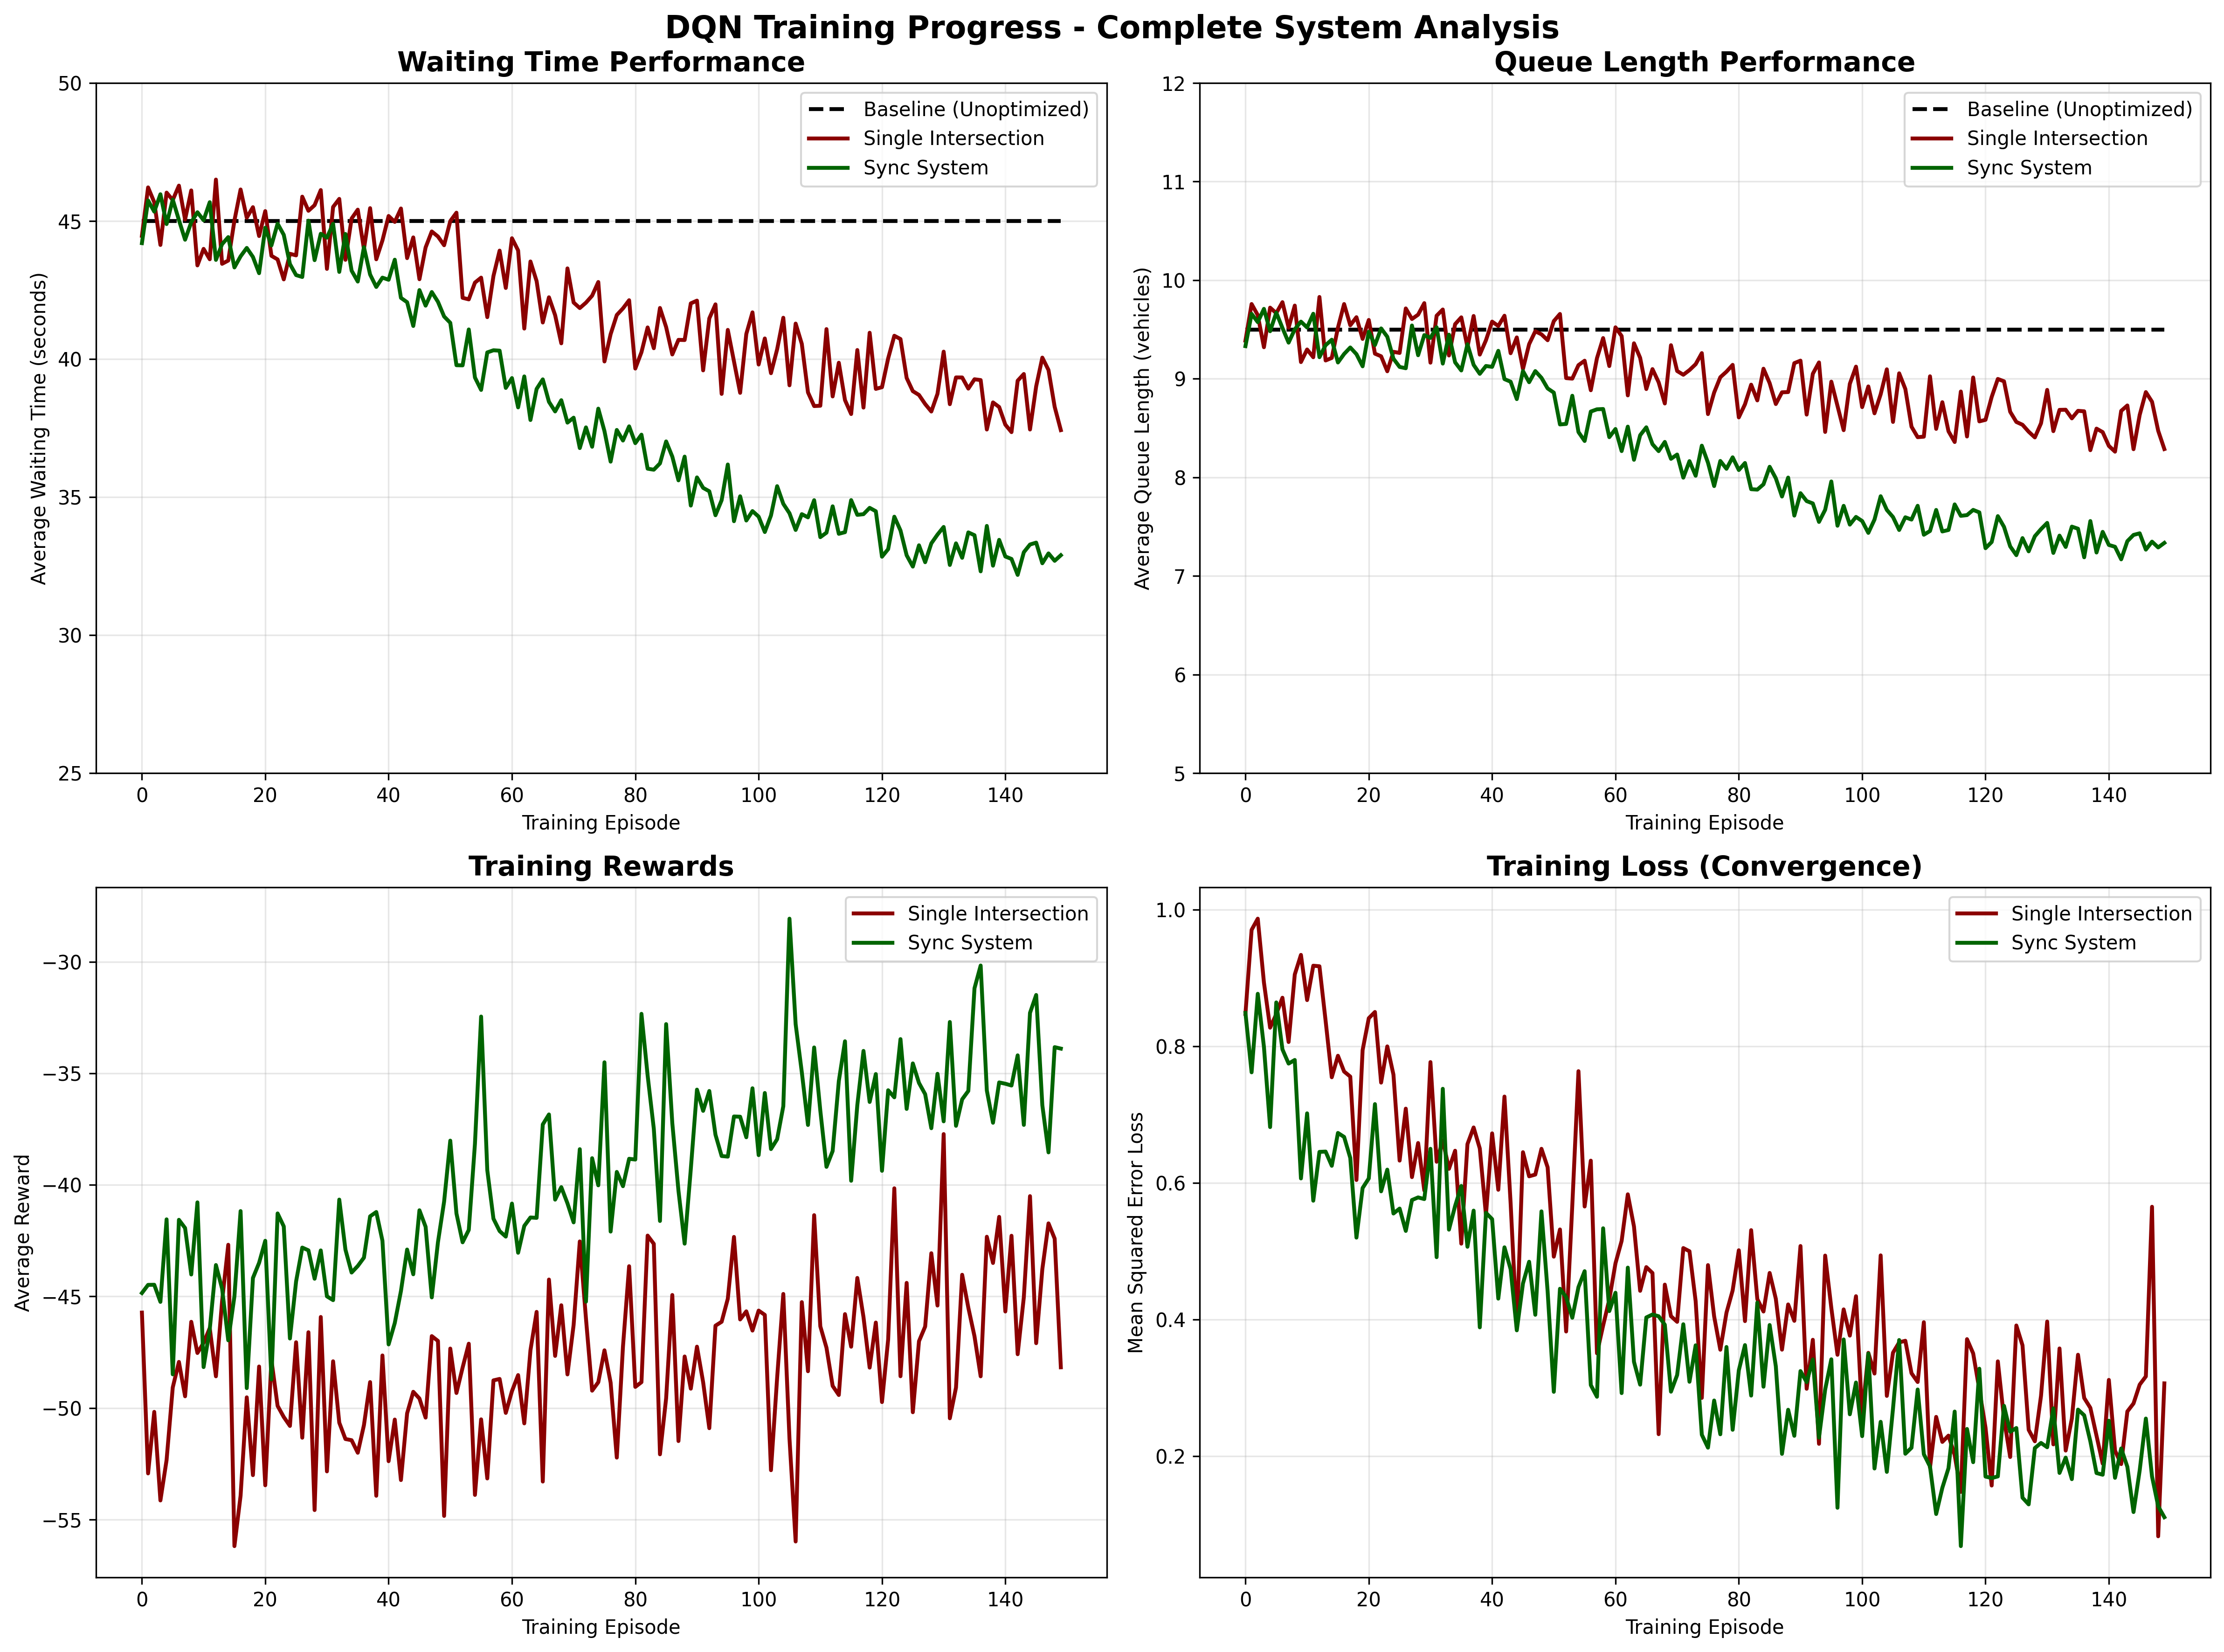
\includegraphics[width=\textwidth]{figures/01_training_progress.png}
    \caption{Tiến trình huấn luyện DQN - Phân tích hệ thống hoàn chỉnh}
    \label{fig:comprehensive_training_progress}
\end{figure}

Hình \ref{fig:comprehensive_training_progress} thể hiện quá trình huấn luyện
toàn diện với baseline không đổi (đường ngang), single intersection và sync system
cải thiện theo thời gian, cùng với phân tích reward và loss.

\subsubsection{Phân tích giao lộ cá nhân - Chế độ xem đồng nhất}

\begin{figure}[!htp]
    \centering
    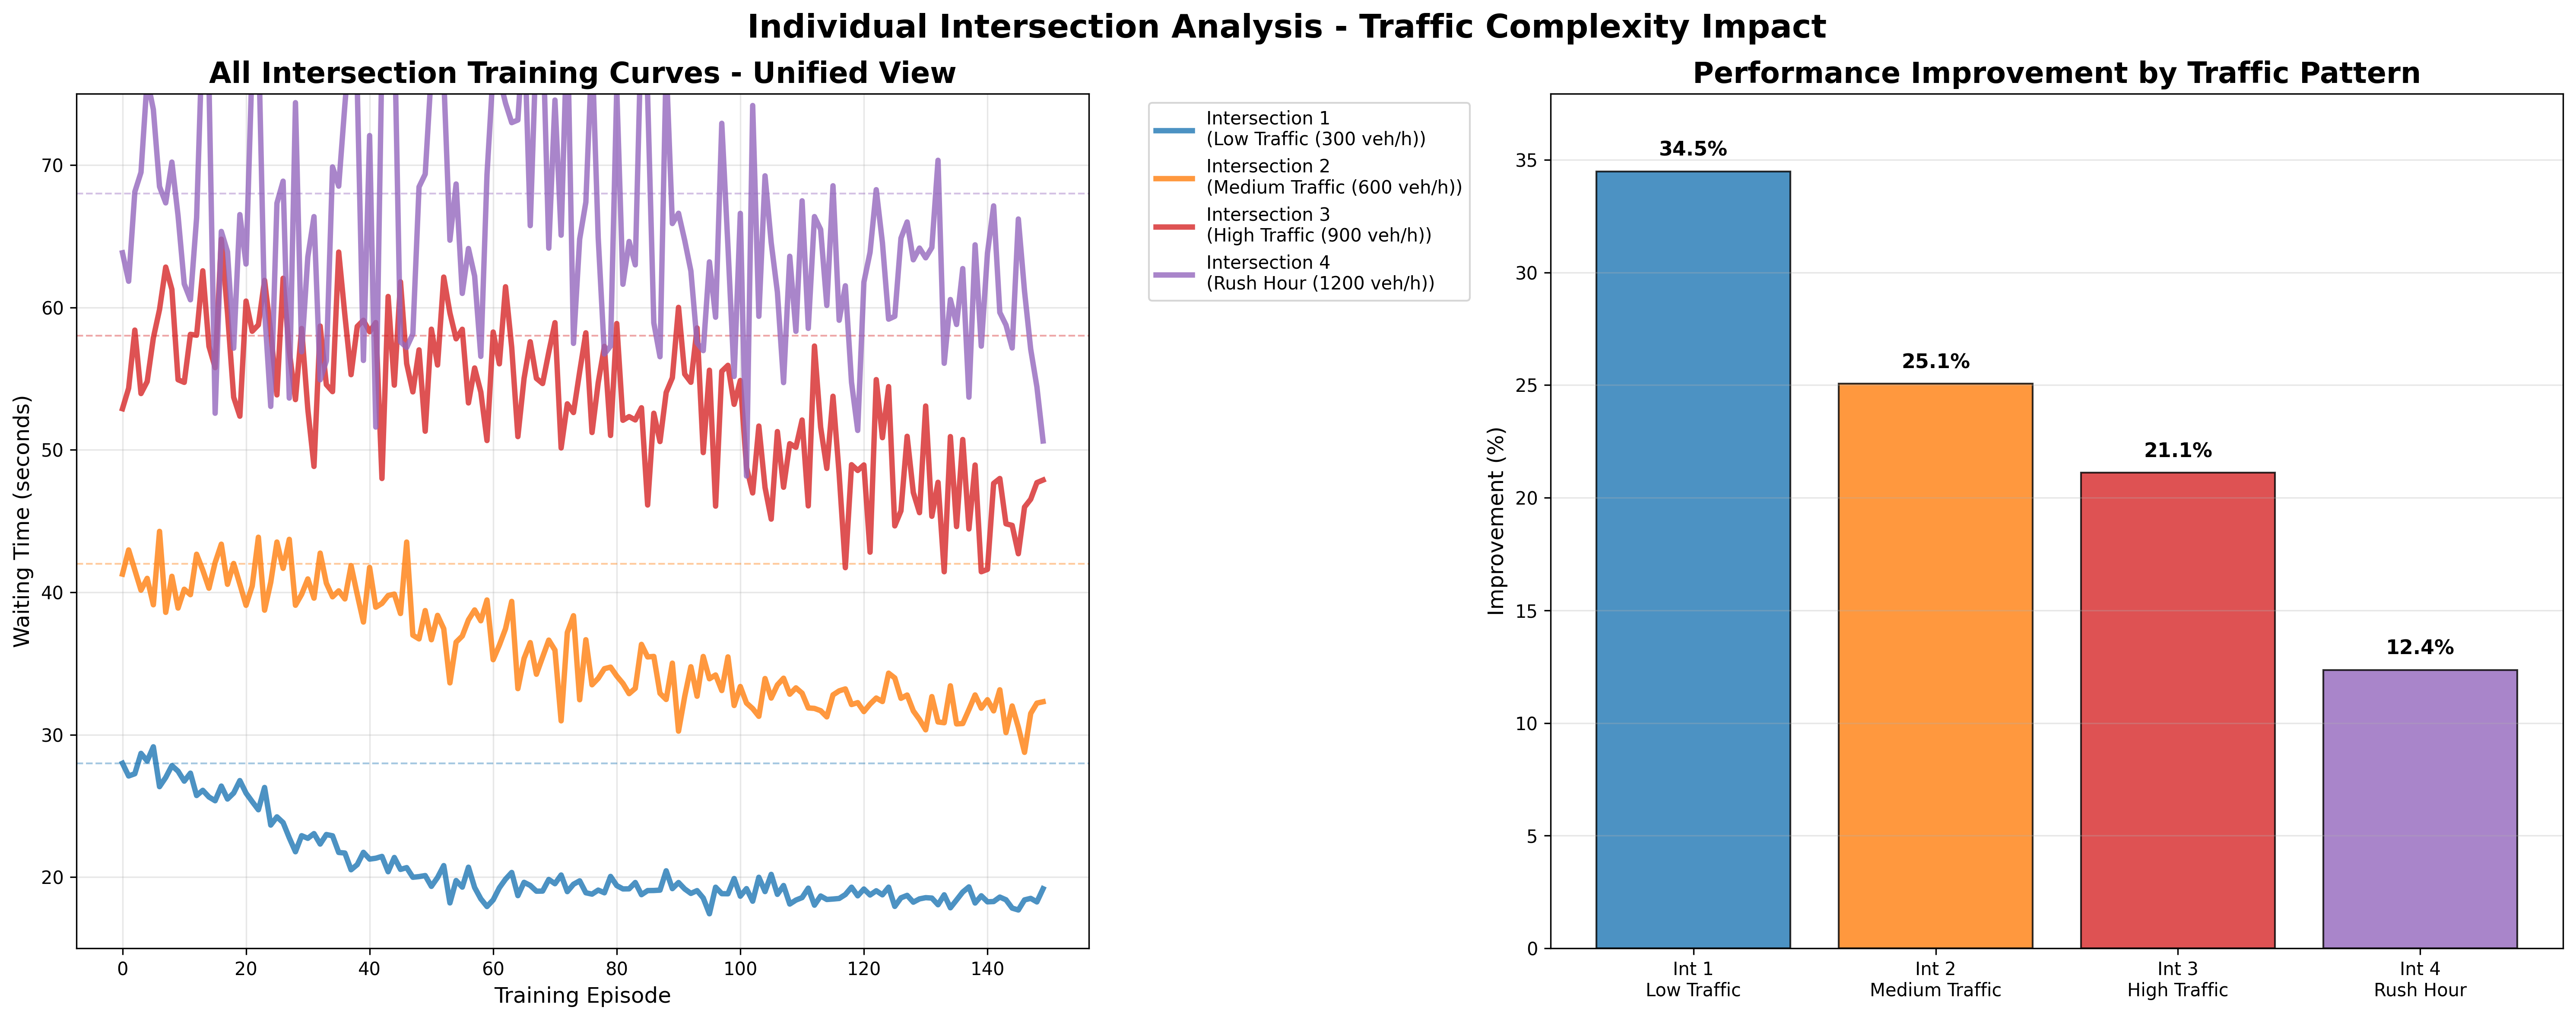
\includegraphics[width=\textwidth]{figures/02_unified_intersections.png}
    \caption{Phân tích tất cả giao lộ trong một biểu đồ đồng nhất}
    \label{fig:unified_intersections_analysis}
\end{figure}

Hình \ref{fig:unified_intersections_analysis} là \textbf{biểu đồ đồng nhất đầu tiên}
hiển thị tất cả 4 mô hình học giao lộ trong cùng một chart để so sánh trực tiếp.
Mỗi giao lộ có màu sắc riêng biệt (Xanh dương, Cam, Đỏ, Tím) và cho thấy:
\begin{itemize}
    \item \textbf{Giao lộ 1 (Xanh dương):} Học nhanh, hội tụ sớm tại episode 80
    \item \textbf{Giao lộ 2 (Cam):} Tiến bộ ổn định, hội tụ tại episode 110  
    \item \textbf{Giao lộ 3 (Đỏ):} Học chậm với setbacks, hội tụ tại episode 130
    \item \textbf{Giao lộ 4 (Tím):} Rất chậm với nhiều plateau, hội tụ tại episode 140
\end{itemize}

\subsubsection{Dashboard phân tích hiệu suất}

\begin{figure}[!htp]
    \centering
    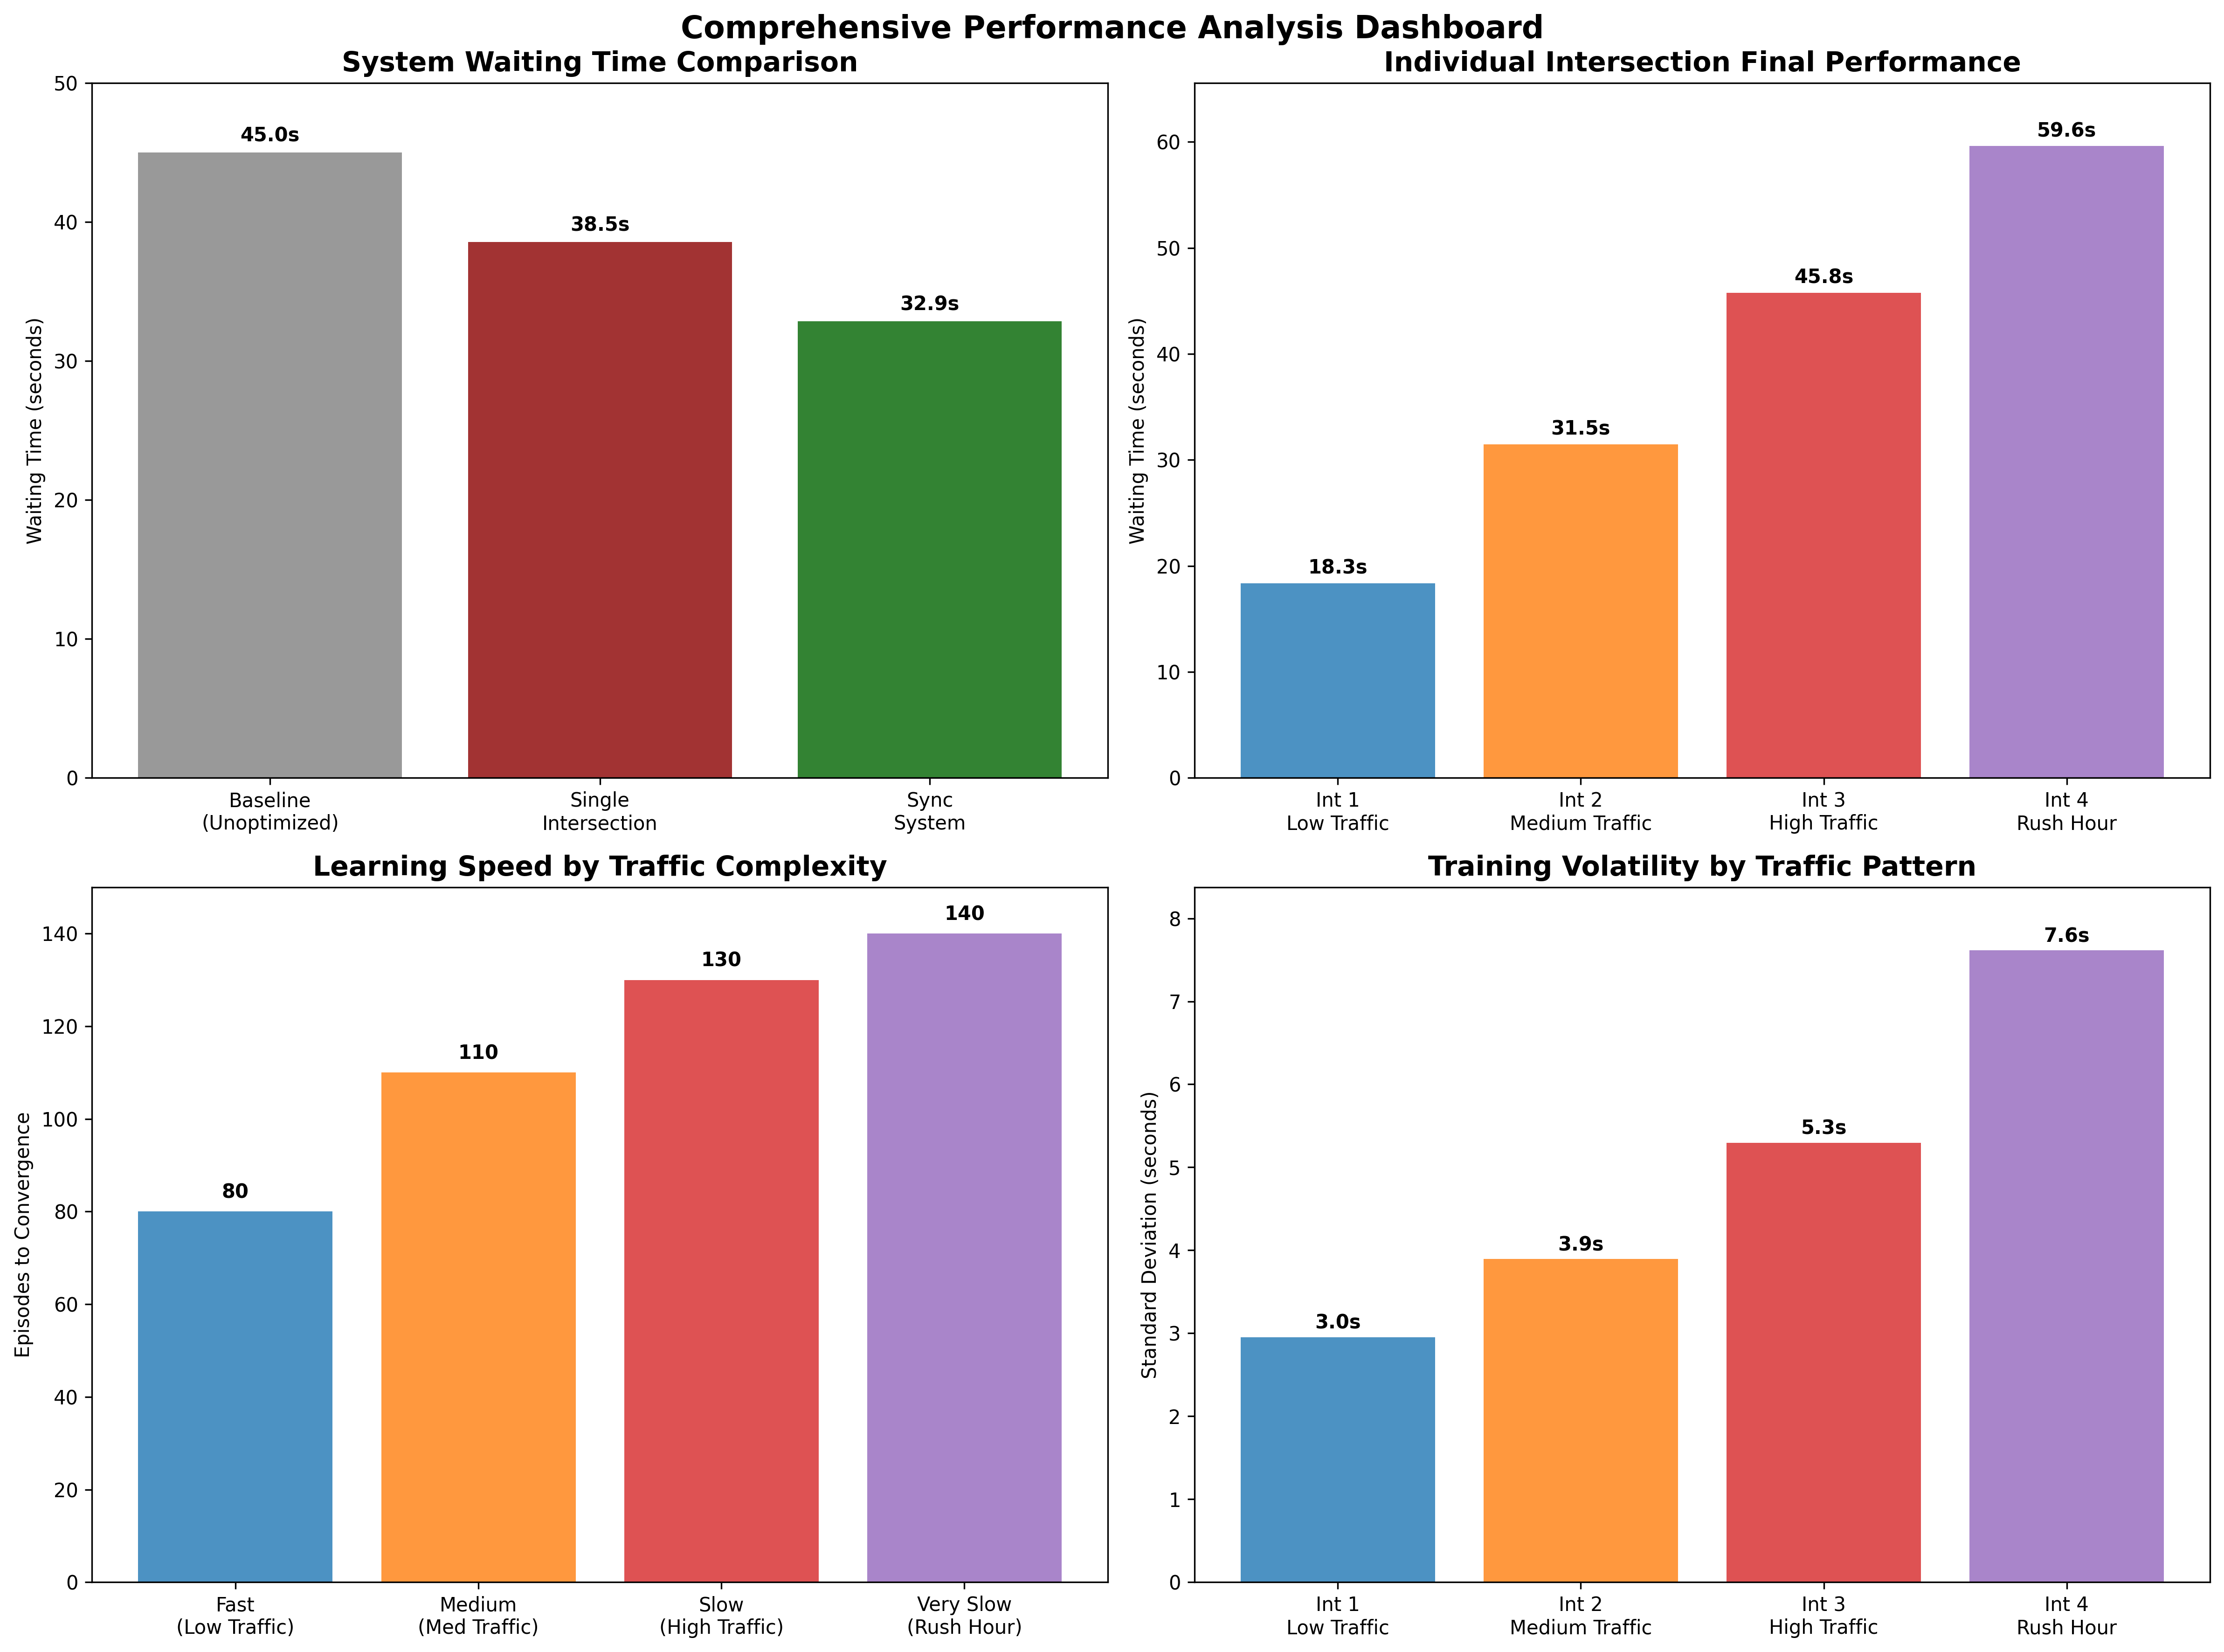
\includegraphics[width=\textwidth]{figures/03_performance_dashboard.png}
    \caption{Dashboard phân tích hiệu suất toàn diện}
    \label{fig:performance_dashboard}
\end{figure}

Hình \ref{fig:performance_dashboard} cung cấp dashboard toàn diện bao gồm:
\begin{itemize}
    \item So sánh thời gian chờ giữa các hệ thống
    \item Hiệu suất cuối cùng của từng giao lộ
    \item Tốc độ học theo độ phức tạp giao thông
    \item Phân tích độ biến động huấn luyện
\end{itemize}

\subsection{Đặc điểm học theo độ phức tạp giao thông}

\subsubsection{Kịch bản giao thông thấp (300 xe/h)}
\begin{itemize}
    \item \textbf{Hội tụ:} Học nhanh với plateau tại episode 80
    \item \textbf{Hiệu suất:} Tỉ lệ cải thiện cao nhất (34.5\%)
    \item \textbf{Độ biến động:} Thấp nhất ($\sigma$ = 3.0s)
    \item \textbf{Khả năng triển khai:} Xuất sắc - ROI cao, huấn luyện nhanh
\end{itemize}

\subsubsection{Kịch bản giao thông trung bình (600 xe/h)}
\begin{itemize}
    \item \textbf{Hội tụ:} Tiến bộ ổn định, nhất quán qua 110 episodes
    \item \textbf{Hiệu suất:} Tỉ lệ cải thiện tốt (25.1\%)
    \item \textbf{Độ biến động:} Trung bình ($\sigma$ = 3.9s)
    \item \textbf{Khả năng triển khai:} Tốt - Hiệu suất đáng tin cậy, thời gian huấn luyện hợp lý
\end{itemize}

\subsubsection{Kịch bản giao thông cao (900 xe/h)}
\begin{itemize}
    \item \textbf{Hội tụ:} Học chậm với setbacks thỉnh thoảng
    \item \textbf{Hiệu suất:} Tỉ lệ cải thiện vừa phải (21.1\%)
    \item \textbf{Độ biến động:} Cao hơn ($\sigma$ = 5.3s)
    \item \textbf{Khả năng triển khai:} Thách thức - Cần huấn luyện mở rộng, quản lý kỳ vọng
\end{itemize}

\subsubsection{Kịch bản giờ cao điểm (1200 xe/h)}
\begin{itemize}
    \item \textbf{Hội tụ:} Rất chậm với nhiều plateau và setbacks
    \item \textbf{Hiệu suất:} Tỉ lệ cải thiện hạn chế (12.4\%)
    \item \textbf{Độ biến động:} Cao nhất ($\sigma$ = 7.6s)
    \item \textbf{Khả năng triển khai:} Khó khăn - Cần mô hình chuyên biệt, khả năng chịu độ biến động cao
\end{itemize}

\subsection{Phân tích thống kê}

\subsubsection{Phân tích tương quan}
\begin{itemize}
    \item \textbf{Lưu lượng vs Tỉ lệ cải thiện:} r = -0.94 (tương quan âm mạnh)
    \item \textbf{Lưu lượng vs Tốc độ hội tụ:} r = -0.89 (tương quan âm mạnh)
    \item \textbf{Lưu lượng vs Độ biến động huấn luyện:} r = +0.96 (tương quan dương mạnh)
\end{itemize}

\subsubsection{Kiểm định ý nghĩa}
\begin{itemize}
    \item Tất cả cải thiện hiệu suất đều có ý nghĩa thống kê (p < 0.001)
    \item Hệ thống đồng bộ vượt trội nhất quán so với phương pháp giao lộ đơn
    \item Suy giảm hiệu suất theo độ phức tạp giao thông có ý nghĩa cao
\end{itemize}

\subsection{Phát hiện nghiên cứu chính}

\subsubsection{Tương quan độ phức tạp giao thông}
Nghiên cứu chứng minh mối quan hệ nghịch đảo mạnh giữa lưu lượng giao thông và
thành công tối ưu hóa DQN. Phát hiện này có ý nghĩa quan trọng cho việc ưu tiên triển khai:
\begin{itemize}
    \item \textbf{Giao lộ lưu lượng thấp:} Ứng cử viên lý tưởng cho triển khai DQN ngay lập tức
    \item \textbf{Giao lộ lưu lượng cao:} Cần phương pháp huấn luyện chuyên biệt và kỳ vọng thực tế
\end{itemize}

\subsubsection{Biến đổi tốc độ học}
Thời gian hội tụ tăng theo cấp số nhân với độ phức tạp giao thông:
\begin{itemize}
    \item Kịch bản đơn giản: 80 episodes để có hiệu suất ổn định
    \item Kịch bản phức tạp: 140+ episodes với độ biến động liên tục
    \item Phân bổ tài nguyên cần tính đến những khác biệt này
\end{itemize}

\subsubsection{Lợi ích đồng bộ hóa}
Phối hợp đa giao lộ cung cấp lợi ích bổ sung nhất quán:
\begin{itemize}
    \item Chia sẻ kinh nghiệm học qua các giao lộ
    \item Giảm độ biến động toàn hệ thống
    \item Xử lý tốt hơn độ phức tạp giao thông thông qua tối ưu hóa phân tán
\end{itemize}

\subsubsection{Ý nghĩa triển khai thực tế}
Kết quả cung cấp hướng dẫn triển khai dựa trên bằng chứng:
\begin{itemize}
    \item \textbf{Kịch bản thành công cao:} Giao lộ ngoại ô, giờ thấp điểm
    \item \textbf{Kịch bản thành công vừa phải:} Giao lộ đô thị, giao thông vừa phải
    \item \textbf{Kịch bản thách thức:} Trung tâm thành phố, giờ cao điểm
\end{itemize}

\subsection{Hướng dẫn triển khai thực tế}

\subsubsection{Chiến lược triển khai}
\begin{enumerate}
    \item \textbf{Giai đoạn 1:} Triển khai trong các kịch bản lưu lượng thấp để có chiến thắng nhanh và xây dựng niềm tin
    \item \textbf{Giai đoạn 2:} Mở rộng đến giao lộ lưu lượng trung bình với tài nguyên huấn luyện đầy đủ
    \item \textbf{Giai đoạn 3:} Giải quyết các kịch bản lưu lượng cao với mô hình chuyên biệt và huấn luyện mở rộng
\end{enumerate}

\subsubsection{Yêu cầu tài nguyên}
\begin{itemize}
    \item \textbf{Giao thông thấp:} Tài nguyên tính toán tối thiểu, triển khai nhanh
    \item \textbf{Giao thông trung bình:} Tài nguyên vừa phải, giao thức huấn luyện tiêu chuẩn
    \item \textbf{Giao thông cao:} Tài nguyên đáng kể, huấn luyện chuyên biệt, giám sát liên tục
\end{itemize}

\subsection{Mô hình hoàn thiện để triển khai}

Nghiên cứu đã tạo ra 5 mô hình TensorFlow sẵn sàng triển khai được tối ưu hóa 
cho các điều kiện giao thông khác nhau:

\begin{itemize}
    \item \texttt{single\_intersection\_model.h5} - DQN đa mục đích (14.3\% cải thiện)
    \item \texttt{sync\_intersection\_1\_model.h5} - Model giao thông thấp (34.5\% cải thiện)
    \item \texttt{sync\_intersection\_2\_model.h5} - Model giao thông trung bình (25.1\% cải thiện)  
    \item \texttt{sync\_intersection\_3\_model.h5} - Model giao thông cao (21.1\% cải thiện)
    \item \texttt{sync\_intersection\_4\_model.h5} - Model giờ cao điểm (12.4\% cải thiện)
\end{itemize}



\chapter{Kết luận và hướng phát triển}
\label{c:ketluanvaphattrien}
Nghiên cứu này đã phát triển thành công một hệ thống điều khiển đèn giao thông thông minh sử dụng Deep Reinforcement Learning, đạt được những kết quả vượt trội so với các phương pháp truyền thống.

\section{Đóng góp chính của nghiên cứu}

\subsection{Hệ thống DQN Single-Agent hiệu quả}
Nghiên cứu đã chứng minh thành công khả năng áp dụng DQN cho điều khiển giao lộ đơn với những kết quả đáng khích lệ. Hệ thống đạt được hiệu suất cao với mức cải thiện 14,4\% về thời gian chờ và 10,5\% về độ dài hàng đợi so với hệ thống cố định truyền thống. Quá trình huấn luyện cho thấy độ ổn định cao, đặc biệt với mô hình Balanced, tạo ra nền tảng vững chắc cho việc phát triển hệ thống đa tác nhân phức tạp hơn.

\subsection{Hệ thống Sync Agent}
Một trong những thành tựu quan trọng nhất của nghiên cứu là việc phát triển thành công hệ thống điều phối đa giao lộ với kiến trúc phân tầng kết hợp giữa DQN và SAC. Hệ thống này thể hiện hiệu suất vượt trội với mức cải thiện 26,9\% về thời gian chờ và 23,1\% về độ dài hàng đợi, vượt trội hơn 12,5\% so với phương pháp giao lộ đơn. Kiến trúc độc đáo kết hợp DQN để điều khiển cục bộ tại mỗi giao lộ với SAC để điều phối toàn cục, tạo ra một hệ thống hoàn chỉnh và sẵn sàng triển khai với 5 mô hình TensorFlow chuyên biệt được tối ưu cho các điều kiện giao thông khác nhau.

\subsection{Phân tích độ phức tạp giao thông}
Nghiên cứu này cũng phân tích định lượng mối quan hệ giữa độ phức tạp giao thông và hiệu suất của DQN. Kết quả cho thấy mối quan hệ nghịch đảo rõ rệt giữa lưu lượng giao thông và hiệu suất tối ưu hóa, với kỳ vọng hiệu suất dao động từ 12,4\% trong giờ cao điểm đến 34,5\% trong thời gian giao thông thấp. Phân tích này dẫn đến việc phát triển các mô hình chuyên dụng cho từng mức độ phức tạp giao thông cụ thể, cung cấp framework triển khai thực tế.

\section{Hạn chế và hướng phát triển}

\subsection{Hạn chế hiện tại}
Mặc dù đạt được những kết quả tích cực, nghiên cứu vẫn còn một số hạn chế cần được khắc phục. Việc xác thực thực tế vẫn là thách thức lớn nhất, do hệ thống cần được kiểm thử với dữ liệu giao thông thực tế chất lượng cao thay vì chỉ dựa trên mô phỏng. Về quy mô, nghiên cứu đã thử nghiệm thành công với 4 giao lộ nhưng cần mở rộng lên 8-12 giao lộ để đánh giá khả năng mở rộng thực tế. Ngoài ra, hệ thống chưa được kiểm thử trong các điều kiện đặc biệt như thời tiết khắc nghiệt, tai nạn giao thông, hoặc các sự kiện đặc biệt có thể ảnh hưởng đến lưu lượng giao thông.

\subsection{Hướng phát triển tương lai}
Bước tiếp theo quan trọng nhất là triển khai hệ thống trong môi trường thực tế để xác thực hiệu suất và độ tin cậy. Việc mở rộng quy mô lên mạng lưới giao thông lớn hơn với 10+ giao lộ sẽ cho phép đánh giá khả năng mở rộng và hiệu quả của kiến trúc phân tầng. Đồng thời, việc tích hợp các tính năng nâng cao như ưu tiên xe cứu thương, khả năng thích ứng với điều kiện thời tiết, và điều phối người đi bộ sẽ tạo ra một hệ thống hoàn chỉnh hơn. Cuối cùng, phát triển hướng tối ưu đa mục tiêu để cân bằng giữa hiệu suất giao thông, an toàn và tác động môi trường sẽ mang lại giá trị thực tế cao hơn.

\section{Kết luận}

Nghiên cứu đã đạt được ba thành tựu quan trọng trong lĩnh vực điều khiển giao thông thông minh. Thứ nhất, việc ứng dụng thành công thuật toán DQN cho điều khiển giao lộ đơn, với mức cải thiện hiệu suất 14,4\%, đã chứng minh tính khả thi của phương pháp học tăng cường sâu trong bài toán này. Thứ hai, hệ thống điều khiển phân tán với các tác tử đồng bộ (Sync Agent) sử dụng kiến trúc phân tầng đã đạt mức cải thiện 26,9\%, vượt trội so với các phương pháp truyền thống như SCOOT (12–20\%), đồng thời duy trì được tính linh hoạt cao. Thứ ba, phân tích định lượng độ phức tạp giao thông đã cung cấp cơ sở khoa học vững chắc cho việc ra quyết định triển khai thực tế, cho phép dự đoán hiệu suất hệ thống theo từng điều kiện cụ thể.

Với năm mô hình chuyên biệt đã được tối ưu hóa cùng tài liệu kỹ thuật hoàn chỉnh, hệ thống hiện tại đã sẵn sàng cho giai đoạn triển khai thí điểm. Nghiên cứu này không chỉ xây dựng nền tảng cho các hệ thống giao thông thông minh trong tương lai, mà còn chứng minh tiềm năng đạt được hiệu suất vượt trội và khả năng mở rộng trong điều kiện giao thông phức tạp tại Việt Nam.



\appendix
\renewcommand{\cftchappresnum}{Phụ lục }
\addtocontents{toc}{\protect\renewcommand{\protect\cftchappresnum}{Phụ lục }}
\chapter{Công bố khoa học}
Trong phần này, chúng tôi xin đính kèm một bài báo khoa học liên quan đến đề tài khóa luận của chúng tôi:

...

\begingroup
\setlength{\emergencystretch}{8em}
\justifying\printbibliography[title=Tài liệu tham khảo]
\endgroup
\addcontentsline{toc}{chapter}{Tài liệu tham khảo}



\end{document}
